\documentclass[twoside]{book}

% Packages required by doxygen
\usepackage{fixltx2e}
\usepackage{calc}
\usepackage{doxygen}
\usepackage[export]{adjustbox} % also loads graphicx
\usepackage{graphicx}
\usepackage[utf8]{inputenc}
\usepackage{makeidx}
\usepackage{multicol}
\usepackage{multirow}
\PassOptionsToPackage{warn}{textcomp}
\usepackage{textcomp}
\usepackage[nointegrals]{wasysym}
\usepackage[table]{xcolor}

% Font selection
\usepackage[T1]{fontenc}
\usepackage[scaled=.90]{helvet}
\usepackage{courier}
\usepackage{amssymb}
\usepackage{sectsty}
\renewcommand{\familydefault}{\sfdefault}
\allsectionsfont{%
  \fontseries{bc}\selectfont%
  \color{darkgray}%
}
\renewcommand{\DoxyLabelFont}{%
  \fontseries{bc}\selectfont%
  \color{darkgray}%
}
\newcommand{\+}{\discretionary{\mbox{\scriptsize$\hookleftarrow$}}{}{}}

% Page & text layout
\usepackage{geometry}
\geometry{%
  a4paper,%
  top=2.5cm,%
  bottom=2.5cm,%
  left=2.5cm,%
  right=2.5cm%
}
\tolerance=750
\hfuzz=15pt
\hbadness=750
\setlength{\emergencystretch}{15pt}
\setlength{\parindent}{0cm}
\setlength{\parskip}{3ex plus 2ex minus 2ex}
\makeatletter
\renewcommand{\paragraph}{%
  \@startsection{paragraph}{4}{0ex}{-1.0ex}{1.0ex}{%
    \normalfont\normalsize\bfseries\SS@parafont%
  }%
}
\renewcommand{\subparagraph}{%
  \@startsection{subparagraph}{5}{0ex}{-1.0ex}{1.0ex}{%
    \normalfont\normalsize\bfseries\SS@subparafont%
  }%
}
\makeatother

% Headers & footers
\usepackage{fancyhdr}
\pagestyle{fancyplain}
\fancyhead[LE]{\fancyplain{}{\bfseries\thepage}}
\fancyhead[CE]{\fancyplain{}{}}
\fancyhead[RE]{\fancyplain{}{\bfseries\leftmark}}
\fancyhead[LO]{\fancyplain{}{\bfseries\rightmark}}
\fancyhead[CO]{\fancyplain{}{}}
\fancyhead[RO]{\fancyplain{}{\bfseries\thepage}}
\fancyfoot[LE]{\fancyplain{}{}}
\fancyfoot[CE]{\fancyplain{}{}}
\fancyfoot[RE]{\fancyplain{}{\bfseries\scriptsize Generated by Doxygen }}
\fancyfoot[LO]{\fancyplain{}{\bfseries\scriptsize Generated by Doxygen }}
\fancyfoot[CO]{\fancyplain{}{}}
\fancyfoot[RO]{\fancyplain{}{}}
\renewcommand{\footrulewidth}{0.4pt}
\renewcommand{\chaptermark}[1]{%
  \markboth{#1}{}%
}
\renewcommand{\sectionmark}[1]{%
  \markright{\thesection\ #1}%
}

% Indices & bibliography
\usepackage{natbib}
\usepackage[titles]{tocloft}
\setcounter{tocdepth}{3}
\setcounter{secnumdepth}{5}
\makeindex

% Hyperlinks (required, but should be loaded last)
\usepackage{ifpdf}
\ifpdf
  \usepackage[pdftex,pagebackref=true]{hyperref}
\else
  \usepackage[ps2pdf,pagebackref=true]{hyperref}
\fi
\hypersetup{%
  colorlinks=true,%
  linkcolor=blue,%
  citecolor=blue,%
  unicode%
}

% Custom commands
\newcommand{\clearemptydoublepage}{%
  \newpage{\pagestyle{empty}\cleardoublepage}%
}

\usepackage{caption}
\captionsetup{labelsep=space,justification=centering,font={bf},singlelinecheck=off,skip=4pt,position=top}

%===== C O N T E N T S =====

\begin{document}

% Titlepage & ToC
\hypersetup{pageanchor=false,
             bookmarksnumbered=true,
             pdfencoding=unicode
            }
\pagenumbering{alph}
\begin{titlepage}
\vspace*{7cm}
\begin{center}%
{\Large C\+M\+S\+C516-\/\+Sem\+Eval2018-\/\+Task6 }\\
\vspace*{1cm}
{\large Generated by Doxygen 1.8.14}\\
\end{center}
\end{titlepage}
\clearemptydoublepage
\pagenumbering{roman}
\tableofcontents
\clearemptydoublepage
\pagenumbering{arabic}
\hypersetup{pageanchor=true}

%--- Begin generated contents ---
\chapter{C\+M\+S\+C516}
\label{md_README}
\Hypertarget{md_README}
\input{md_README}
\chapter{Namespace Index}
\section{Namespace List}
Here is a list of all namespaces with brief descriptions\+:\begin{DoxyCompactList}
\item\contentsline{section}{\hyperlink{namespacesetup}{setup} }{\pageref{namespacesetup}}{}
\item\contentsline{section}{\hyperlink{namespacetask6}{task6} }{\pageref{namespacetask6}}{}
\item\contentsline{section}{\hyperlink{namespacetask6_1_1sutime}{task6.\+sutime} }{\pageref{namespacetask6_1_1sutime}}{}
\item\contentsline{section}{\hyperlink{namespacetask6_1_1sutime__wrapper}{task6.\+sutime\+\_\+wrapper} }{\pageref{namespacetask6_1_1sutime__wrapper}}{}
\item\contentsline{section}{\hyperlink{namespacetask6_1_1t6Entities}{task6.\+t6\+Entities} }{\pageref{namespacetask6_1_1t6Entities}}{}
\item\contentsline{section}{\hyperlink{namespacetask6_1_1utils}{task6.\+utils} }{\pageref{namespacetask6_1_1utils}}{}
\item\contentsline{section}{\hyperlink{namespacetest}{test} }{\pageref{namespacetest}}{}
\item\contentsline{section}{\hyperlink{namespacetest_1_1test}{test.\+test} }{\pageref{namespacetest_1_1test}}{}
\end{DoxyCompactList}

\chapter{Hierarchical Index}
\section{Class Hierarchy}
This inheritance list is sorted roughly, but not completely, alphabetically\+:\begin{DoxyCompactList}
\item object\begin{DoxyCompactList}
\item \contentsline{section}{task6.\+sutime.\+S\+U\+Time}{\pageref{classtask6_1_1sutime_1_1SUTime}}{}
\end{DoxyCompactList}
\item \contentsline{section}{task6.\+t6\+Entities.\+t6\+Entity}{\pageref{classtask6_1_1t6Entities_1_1t6Entity}}{}
\begin{DoxyCompactList}
\item \contentsline{section}{task6.\+t6\+Entities.\+t6\+Interval\+Entity}{\pageref{classtask6_1_1t6Entities_1_1t6IntervalEntity}}{}
\item \contentsline{section}{task6.\+t6\+Entities.\+t6\+Operator}{\pageref{classtask6_1_1t6Entities_1_1t6Operator}}{}
\item \contentsline{section}{task6.\+t6\+Entities.\+t6\+Period\+Entity}{\pageref{classtask6_1_1t6Entities_1_1t6PeriodEntity}}{}
\item \contentsline{section}{task6.\+t6\+Entities.\+t6\+Repeating\+Interval\+Entity}{\pageref{classtask6_1_1t6Entities_1_1t6RepeatingIntervalEntity}}{}
\end{DoxyCompactList}
\end{DoxyCompactList}

\chapter{Class Index}
\section{Class List}
Here are the classes, structs, unions and interfaces with brief descriptions\+:\begin{DoxyCompactList}
\item\contentsline{section}{\hyperlink{classtask6_1_1sutime_1_1SUTime}{task6.\+sutime.\+S\+U\+Time} }{\pageref{classtask6_1_1sutime_1_1SUTime}}{}
\item\contentsline{section}{\hyperlink{classtask6_1_1t6Entities_1_1T6AfterOperator}{task6.\+t6\+Entities.\+T6\+After\+Operator} }{\pageref{classtask6_1_1t6Entities_1_1T6AfterOperator}}{}
\item\contentsline{section}{\hyperlink{classtask6_1_1t6Entities_1_1T6AMPMOfDay}{task6.\+t6\+Entities.\+T6\+A\+M\+P\+M\+Of\+Day} }{\pageref{classtask6_1_1t6Entities_1_1T6AMPMOfDay}}{}
\item\contentsline{section}{\hyperlink{classtask6_1_1t6Entities_1_1T6BeforeOperator}{task6.\+t6\+Entities.\+T6\+Before\+Operator} }{\pageref{classtask6_1_1t6Entities_1_1T6BeforeOperator}}{}
\item\contentsline{section}{\hyperlink{classtask6_1_1t6Entities_1_1T6BetweenOperator}{task6.\+t6\+Entities.\+T6\+Between\+Operator} }{\pageref{classtask6_1_1t6Entities_1_1T6BetweenOperator}}{}
\item\contentsline{section}{\hyperlink{classtask6_1_1t6Entities_1_1T6CalendarIntervalEntity}{task6.\+t6\+Entities.\+T6\+Calendar\+Interval\+Entity} }{\pageref{classtask6_1_1t6Entities_1_1T6CalendarIntervalEntity}}{}
\item\contentsline{section}{\hyperlink{classtask6_1_1t6Entities_1_1T6DayOfMonthEntity}{task6.\+t6\+Entities.\+T6\+Day\+Of\+Month\+Entity} }{\pageref{classtask6_1_1t6Entities_1_1T6DayOfMonthEntity}}{}
\item\contentsline{section}{\hyperlink{classtask6_1_1t6Entities_1_1T6DayOfWeekEntity}{task6.\+t6\+Entities.\+T6\+Day\+Of\+Week\+Entity} }{\pageref{classtask6_1_1t6Entities_1_1T6DayOfWeekEntity}}{}
\item\contentsline{section}{\hyperlink{classtask6_1_1t6Entities_1_1T6DifferenceOperator}{task6.\+t6\+Entities.\+T6\+Difference\+Operator} }{\pageref{classtask6_1_1t6Entities_1_1T6DifferenceOperator}}{}
\item\contentsline{section}{\hyperlink{classtask6_1_1t6Entities_1_1T6Entity}{task6.\+t6\+Entities.\+T6\+Entity} \\*Class definitions for all Time\+Norm entities -\/ Intervals, Periods, Repeating-\/\+Intervals, and Operators }{\pageref{classtask6_1_1t6Entities_1_1T6Entity}}{}
\item\contentsline{section}{\hyperlink{classtask6_1_1t6Entities_1_1T6Event}{task6.\+t6\+Entities.\+T6\+Event} }{\pageref{classtask6_1_1t6Entities_1_1T6Event}}{}
\item\contentsline{section}{\hyperlink{classtask6_1_1t6Entities_1_1T6EveryNthOperator}{task6.\+t6\+Entities.\+T6\+Every\+Nth\+Operator} }{\pageref{classtask6_1_1t6Entities_1_1T6EveryNthOperator}}{}
\item\contentsline{section}{\hyperlink{classtask6_1_1t6Entities_1_1T6HourOfDayEntity}{task6.\+t6\+Entities.\+T6\+Hour\+Of\+Day\+Entity} }{\pageref{classtask6_1_1t6Entities_1_1T6HourOfDayEntity}}{}
\item\contentsline{section}{\hyperlink{classtask6_1_1t6Entities_1_1T6IntersectionOperator}{task6.\+t6\+Entities.\+T6\+Intersection\+Operator} }{\pageref{classtask6_1_1t6Entities_1_1T6IntersectionOperator}}{}
\item\contentsline{section}{\hyperlink{classtask6_1_1t6Entities_1_1T6IntervalEntity}{task6.\+t6\+Entities.\+T6\+Interval\+Entity} \\*An interval, just super classes for year interval for consistency }{\pageref{classtask6_1_1t6Entities_1_1T6IntervalEntity}}{}
\item\contentsline{section}{\hyperlink{classtask6_1_1t6Entities_1_1T6LastOperator}{task6.\+t6\+Entities.\+T6\+Last\+Operator} \\*Create a last(\+Period) or last(Repeating-\/\+Interval) operator }{\pageref{classtask6_1_1t6Entities_1_1T6LastOperator}}{}
\item\contentsline{section}{\hyperlink{classtask6_1_1t6Entities_1_1T6MinuteOfHourEntity}{task6.\+t6\+Entities.\+T6\+Minute\+Of\+Hour\+Entity} }{\pageref{classtask6_1_1t6Entities_1_1T6MinuteOfHourEntity}}{}
\item\contentsline{section}{\hyperlink{classtask6_1_1t6Entities_1_1T6Modifier}{task6.\+t6\+Entities.\+T6\+Modifier} }{\pageref{classtask6_1_1t6Entities_1_1T6Modifier}}{}
\item\contentsline{section}{\hyperlink{classtask6_1_1t6Entities_1_1T6MonthOfYearEntity}{task6.\+t6\+Entities.\+T6\+Month\+Of\+Year\+Entity} }{\pageref{classtask6_1_1t6Entities_1_1T6MonthOfYearEntity}}{}
\item\contentsline{section}{\hyperlink{classtask6_1_1t6Entities_1_1T6NextOperator}{task6.\+t6\+Entities.\+T6\+Next\+Operator} }{\pageref{classtask6_1_1t6Entities_1_1T6NextOperator}}{}
\item\contentsline{section}{\hyperlink{classtask6_1_1t6Entities_1_1T6NthOperator}{task6.\+t6\+Entities.\+T6\+Nth\+Operator} }{\pageref{classtask6_1_1t6Entities_1_1T6NthOperator}}{}
\item\contentsline{section}{\hyperlink{classtask6_1_1t6Entities_1_1T6Number}{task6.\+t6\+Entities.\+T6\+Number} }{\pageref{classtask6_1_1t6Entities_1_1T6Number}}{}
\item\contentsline{section}{\hyperlink{classtask6_1_1t6Entities_1_1T6Operator}{task6.\+t6\+Entities.\+T6\+Operator} }{\pageref{classtask6_1_1t6Entities_1_1T6Operator}}{}
\item\contentsline{section}{\hyperlink{classtask6_1_1t6Entities_1_1T6PartOfDayEntity}{task6.\+t6\+Entities.\+T6\+Part\+Of\+Day\+Entity} }{\pageref{classtask6_1_1t6Entities_1_1T6PartOfDayEntity}}{}
\item\contentsline{section}{\hyperlink{classtask6_1_1t6Entities_1_1T6PeriodEntity}{task6.\+t6\+Entities.\+T6\+Period\+Entity} }{\pageref{classtask6_1_1t6Entities_1_1T6PeriodEntity}}{}
\item\contentsline{section}{\hyperlink{classtask6_1_1t6Entities_1_1T6repeatingIntervalEntity}{task6.\+t6\+Entities.\+T6repeating\+Interval\+Entity} }{\pageref{classtask6_1_1t6Entities_1_1T6repeatingIntervalEntity}}{}
\item\contentsline{section}{\hyperlink{classtask6_1_1t6Entities_1_1T6SecondOfMinuteEntity}{task6.\+t6\+Entities.\+T6\+Second\+Of\+Minute\+Entity} }{\pageref{classtask6_1_1t6Entities_1_1T6SecondOfMinuteEntity}}{}
\item\contentsline{section}{\hyperlink{classtask6_1_1t6Entities_1_1T6SumOperator}{task6.\+t6\+Entities.\+T6\+Sum\+Operator} }{\pageref{classtask6_1_1t6Entities_1_1T6SumOperator}}{}
\item\contentsline{section}{\hyperlink{classtask6_1_1t6Entities_1_1T6ThisOperator}{task6.\+t6\+Entities.\+T6\+This\+Operator} }{\pageref{classtask6_1_1t6Entities_1_1T6ThisOperator}}{}
\item\contentsline{section}{\hyperlink{classtask6_1_1t6Entities_1_1T6time__zoneEntity}{task6.\+t6\+Entities.\+T6time\+\_\+zone\+Entity} }{\pageref{classtask6_1_1t6Entities_1_1T6time__zoneEntity}}{}
\item\contentsline{section}{\hyperlink{classtask6_1_1t6Entities_1_1T6TwoDigitYearOperator}{task6.\+t6\+Entities.\+T6\+Two\+Digit\+Year\+Operator} }{\pageref{classtask6_1_1t6Entities_1_1T6TwoDigitYearOperator}}{}
\item\contentsline{section}{\hyperlink{classtask6_1_1t6Entities_1_1T6UnionOperator}{task6.\+t6\+Entities.\+T6\+Union\+Operator} }{\pageref{classtask6_1_1t6Entities_1_1T6UnionOperator}}{}
\item\contentsline{section}{\hyperlink{classtask6_1_1t6Entities_1_1T6WeekOfYearEntity}{task6.\+t6\+Entities.\+T6\+Week\+Of\+Year\+Entity} }{\pageref{classtask6_1_1t6Entities_1_1T6WeekOfYearEntity}}{}
\item\contentsline{section}{\hyperlink{classtask6_1_1t6Entities_1_1T6YearEntity}{task6.\+t6\+Entities.\+T6\+Year\+Entity} \\*A year interval }{\pageref{classtask6_1_1t6Entities_1_1T6YearEntity}}{}
\end{DoxyCompactList}

\chapter{File Index}
\section{File List}
Here is a list of all files with brief descriptions\+:\begin{DoxyCompactList}
\item\contentsline{section}{\hyperlink{setup_8py}{setup.\+py} }{\pageref{setup_8py}}{}
\item\contentsline{section}{\hyperlink{test_8py}{test.\+py} }{\pageref{test_8py}}{}
\item\contentsline{section}{task6/\hyperlink{task6_2____init_____8py}{\+\_\+\+\_\+init\+\_\+\+\_\+.\+py} }{\pageref{task6_2____init_____8py}}{}
\item\contentsline{section}{task6/\hyperlink{sutime_8py}{sutime.\+py} }{\pageref{sutime_8py}}{}
\item\contentsline{section}{task6/\hyperlink{sutime__wrapper_8py}{sutime\+\_\+wrapper.\+py} }{\pageref{sutime__wrapper_8py}}{}
\item\contentsline{section}{task6/\hyperlink{t6Entities_8py}{t6\+Entities.\+py} }{\pageref{t6Entities_8py}}{}
\item\contentsline{section}{task6/\hyperlink{utils_8py}{utils.\+py} }{\pageref{utils_8py}}{}
\item\contentsline{section}{test/\hyperlink{test_2____init_____8py}{\+\_\+\+\_\+init\+\_\+\+\_\+.\+py} }{\pageref{test_2____init_____8py}}{}
\item\contentsline{section}{test/\hyperlink{test_2test_8py}{test.\+py} }{\pageref{test_2test_8py}}{}
\end{DoxyCompactList}

\chapter{Namespace Documentation}
\hypertarget{namespacesetup}{}\section{setup Namespace Reference}
\label{namespacesetup}\index{setup@{setup}}
\subsection*{Variables}
\begin{DoxyCompactItemize}
\item 
\hyperlink{namespacesetup_a9c076537d899ffd8096e58c282bb7b02}{here} = path.\+abspath(path.\+dirname(\+\_\+\+\_\+file\+\_\+\+\_\+))
\item 
\hyperlink{namespacesetup_a443be2d01fd539bf6761aff70724d876}{encoding}
\item 
\hyperlink{namespacesetup_a4cda9dbfb952875376a0749fe08a5bde}{long\+\_\+description} = f.\+read()
\item 
\hyperlink{namespacesetup_ab3a7a0638d76a01367c5bc3cc699447f}{name}
\item 
\hyperlink{namespacesetup_a2aa722b36a933088812b50ea79b97a5c}{version}
\item 
\hyperlink{namespacesetup_aedf461ec52a946bda975938ba0b93ec0}{description}
\item 
\hyperlink{namespacesetup_afc13124aa5c0124e84e1d965e3f4b0fb}{url}
\item 
\hyperlink{namespacesetup_a3a57a4772d418a06835249cbade0d86a}{author}
\item 
\hyperlink{namespacesetup_a5b08034343aa2be607722a8b315f3625}{author\+\_\+email}
\item 
\hyperlink{namespacesetup_a8ed6f50a28bd6a8794f8e1153baa6de9}{license}
\item 
\hyperlink{namespacesetup_abe96a9c38c1c61f9f0fdb002c482f785}{classifiers}
\item 
\hyperlink{namespacesetup_a73ae9ecb109f0dcab6f0b6a89043c5c3}{keywords}
\item 
\hyperlink{namespacesetup_aff2375a361fd5865c77bd9aa093be747}{packages}
\item 
\hyperlink{namespacesetup_abead4f26b530856f858f0d44c7cf2588}{install\+\_\+requires}
\end{DoxyCompactItemize}


\subsection{Variable Documentation}
\mbox{\Hypertarget{namespacesetup_a3a57a4772d418a06835249cbade0d86a}\label{namespacesetup_a3a57a4772d418a06835249cbade0d86a}} 
\index{setup@{setup}!author@{author}}
\index{author@{author}!setup@{setup}}
\subsubsection{\texorpdfstring{author}{author}}
{\footnotesize\ttfamily setup.\+author}

\mbox{\Hypertarget{namespacesetup_a5b08034343aa2be607722a8b315f3625}\label{namespacesetup_a5b08034343aa2be607722a8b315f3625}} 
\index{setup@{setup}!author\+\_\+email@{author\+\_\+email}}
\index{author\+\_\+email@{author\+\_\+email}!setup@{setup}}
\subsubsection{\texorpdfstring{author\+\_\+email}{author\_email}}
{\footnotesize\ttfamily setup.\+author\+\_\+email}

\mbox{\Hypertarget{namespacesetup_abe96a9c38c1c61f9f0fdb002c482f785}\label{namespacesetup_abe96a9c38c1c61f9f0fdb002c482f785}} 
\index{setup@{setup}!classifiers@{classifiers}}
\index{classifiers@{classifiers}!setup@{setup}}
\subsubsection{\texorpdfstring{classifiers}{classifiers}}
{\footnotesize\ttfamily setup.\+classifiers}

\mbox{\Hypertarget{namespacesetup_aedf461ec52a946bda975938ba0b93ec0}\label{namespacesetup_aedf461ec52a946bda975938ba0b93ec0}} 
\index{setup@{setup}!description@{description}}
\index{description@{description}!setup@{setup}}
\subsubsection{\texorpdfstring{description}{description}}
{\footnotesize\ttfamily setup.\+description}

\mbox{\Hypertarget{namespacesetup_a443be2d01fd539bf6761aff70724d876}\label{namespacesetup_a443be2d01fd539bf6761aff70724d876}} 
\index{setup@{setup}!encoding@{encoding}}
\index{encoding@{encoding}!setup@{setup}}
\subsubsection{\texorpdfstring{encoding}{encoding}}
{\footnotesize\ttfamily setup.\+encoding}

\mbox{\Hypertarget{namespacesetup_a9c076537d899ffd8096e58c282bb7b02}\label{namespacesetup_a9c076537d899ffd8096e58c282bb7b02}} 
\index{setup@{setup}!here@{here}}
\index{here@{here}!setup@{setup}}
\subsubsection{\texorpdfstring{here}{here}}
{\footnotesize\ttfamily setup.\+here = path.\+abspath(path.\+dirname(\+\_\+\+\_\+file\+\_\+\+\_\+))}

\mbox{\Hypertarget{namespacesetup_abead4f26b530856f858f0d44c7cf2588}\label{namespacesetup_abead4f26b530856f858f0d44c7cf2588}} 
\index{setup@{setup}!install\+\_\+requires@{install\+\_\+requires}}
\index{install\+\_\+requires@{install\+\_\+requires}!setup@{setup}}
\subsubsection{\texorpdfstring{install\+\_\+requires}{install\_requires}}
{\footnotesize\ttfamily setup.\+install\+\_\+requires}

\mbox{\Hypertarget{namespacesetup_a73ae9ecb109f0dcab6f0b6a89043c5c3}\label{namespacesetup_a73ae9ecb109f0dcab6f0b6a89043c5c3}} 
\index{setup@{setup}!keywords@{keywords}}
\index{keywords@{keywords}!setup@{setup}}
\subsubsection{\texorpdfstring{keywords}{keywords}}
{\footnotesize\ttfamily setup.\+keywords}

\mbox{\Hypertarget{namespacesetup_a8ed6f50a28bd6a8794f8e1153baa6de9}\label{namespacesetup_a8ed6f50a28bd6a8794f8e1153baa6de9}} 
\index{setup@{setup}!license@{license}}
\index{license@{license}!setup@{setup}}
\subsubsection{\texorpdfstring{license}{license}}
{\footnotesize\ttfamily setup.\+license}

\mbox{\Hypertarget{namespacesetup_a4cda9dbfb952875376a0749fe08a5bde}\label{namespacesetup_a4cda9dbfb952875376a0749fe08a5bde}} 
\index{setup@{setup}!long\+\_\+description@{long\+\_\+description}}
\index{long\+\_\+description@{long\+\_\+description}!setup@{setup}}
\subsubsection{\texorpdfstring{long\+\_\+description}{long\_description}}
{\footnotesize\ttfamily setup.\+long\+\_\+description = f.\+read()}

\mbox{\Hypertarget{namespacesetup_ab3a7a0638d76a01367c5bc3cc699447f}\label{namespacesetup_ab3a7a0638d76a01367c5bc3cc699447f}} 
\index{setup@{setup}!name@{name}}
\index{name@{name}!setup@{setup}}
\subsubsection{\texorpdfstring{name}{name}}
{\footnotesize\ttfamily setup.\+name}

\mbox{\Hypertarget{namespacesetup_aff2375a361fd5865c77bd9aa093be747}\label{namespacesetup_aff2375a361fd5865c77bd9aa093be747}} 
\index{setup@{setup}!packages@{packages}}
\index{packages@{packages}!setup@{setup}}
\subsubsection{\texorpdfstring{packages}{packages}}
{\footnotesize\ttfamily setup.\+packages}

\mbox{\Hypertarget{namespacesetup_afc13124aa5c0124e84e1d965e3f4b0fb}\label{namespacesetup_afc13124aa5c0124e84e1d965e3f4b0fb}} 
\index{setup@{setup}!url@{url}}
\index{url@{url}!setup@{setup}}
\subsubsection{\texorpdfstring{url}{url}}
{\footnotesize\ttfamily setup.\+url}

\mbox{\Hypertarget{namespacesetup_a2aa722b36a933088812b50ea79b97a5c}\label{namespacesetup_a2aa722b36a933088812b50ea79b97a5c}} 
\index{setup@{setup}!version@{version}}
\index{version@{version}!setup@{setup}}
\subsubsection{\texorpdfstring{version}{version}}
{\footnotesize\ttfamily setup.\+version}


\hypertarget{namespacetask6}{}\section{task6 Namespace Reference}
\label{namespacetask6}\index{task6@{task6}}
\subsection*{Namespaces}
\begin{DoxyCompactItemize}
\item 
 \hyperlink{namespacetask6_1_1sutime}{sutime}
\item 
 \hyperlink{namespacetask6_1_1sutime__wrapper}{sutime\+\_\+wrapper}
\item 
 \hyperlink{namespacetask6_1_1t6Entities}{t6\+Entities}
\item 
 \hyperlink{namespacetask6_1_1utils}{utils}
\end{DoxyCompactItemize}

\hypertarget{namespacetask6_1_1sutime}{}\section{task6.\+sutime Namespace Reference}
\label{namespacetask6_1_1sutime}\index{task6.\+sutime@{task6.\+sutime}}
\subsection*{Classes}
\begin{DoxyCompactItemize}
\item 
class \hyperlink{classtask6_1_1sutime_1_1SUTime}{S\+U\+Time}
\end{DoxyCompactItemize}

\hypertarget{namespacetask6_1_1sutime__wrapper}{}\section{task6.\+sutime\+\_\+wrapper Namespace Reference}
\label{namespacetask6_1_1sutime__wrapper}\index{task6.\+sutime\+\_\+wrapper@{task6.\+sutime\+\_\+wrapper}}
\subsection*{Functions}
\begin{DoxyCompactItemize}
\item 
def \hyperlink{namespacetask6_1_1sutime__wrapper_af4cac751d594757efbe539a28850ff28}{call\+S\+U\+Time\+Parse} (file\+\_\+path)
\begin{DoxyCompactList}\small\item\em call\+S\+U\+T\+I\+M\+E\+Parse() Function Purpose\+: Takes in raw text file and performs S\+U\+Time\textquotesingle{}s algorithm on \#it and returns it in J\+S\+ON format. \end{DoxyCompactList}\end{DoxyCompactItemize}


\subsection{Function Documentation}
\mbox{\Hypertarget{namespacetask6_1_1sutime__wrapper_af4cac751d594757efbe539a28850ff28}\label{namespacetask6_1_1sutime__wrapper_af4cac751d594757efbe539a28850ff28}} 
\index{task6\+::sutime\+\_\+wrapper@{task6\+::sutime\+\_\+wrapper}!call\+S\+U\+Time\+Parse@{call\+S\+U\+Time\+Parse}}
\index{call\+S\+U\+Time\+Parse@{call\+S\+U\+Time\+Parse}!task6\+::sutime\+\_\+wrapper@{task6\+::sutime\+\_\+wrapper}}
\subsubsection{\texorpdfstring{call\+S\+U\+Time\+Parse()}{callSUTimeParse()}}
{\footnotesize\ttfamily def task6.\+sutime\+\_\+wrapper.\+call\+S\+U\+Time\+Parse (\begin{DoxyParamCaption}\item[{}]{file\+\_\+path }\end{DoxyParamCaption})}



call\+S\+U\+T\+I\+M\+E\+Parse() Function Purpose\+: Takes in raw text file and performs S\+U\+Time\textquotesingle{}s algorithm on \#it and returns it in J\+S\+ON format. 

Input\+: String containing the location and name of the text file to be parsed. Output\+: J\+S\+ON string output of raw input file 
\hypertarget{namespacetask6_1_1t6Entities}{}\section{task6.\+t6\+Entities Namespace Reference}
\label{namespacetask6_1_1t6Entities}\index{task6.\+t6\+Entities@{task6.\+t6\+Entities}}
\subsection*{Classes}
\begin{DoxyCompactItemize}
\item 
class \hyperlink{classtask6_1_1t6Entities_1_1T6AfterOperator}{T6\+After\+Operator}
\item 
class \hyperlink{classtask6_1_1t6Entities_1_1T6AMPMOfDay}{T6\+A\+M\+P\+M\+Of\+Day}
\item 
class \hyperlink{classtask6_1_1t6Entities_1_1T6BeforeOperator}{T6\+Before\+Operator}
\item 
class \hyperlink{classtask6_1_1t6Entities_1_1T6BetweenOperator}{T6\+Between\+Operator}
\item 
class \hyperlink{classtask6_1_1t6Entities_1_1T6CalendarIntervalEntity}{T6\+Calendar\+Interval\+Entity}
\item 
class \hyperlink{classtask6_1_1t6Entities_1_1T6DayOfMonthEntity}{T6\+Day\+Of\+Month\+Entity}
\item 
class \hyperlink{classtask6_1_1t6Entities_1_1T6DayOfWeekEntity}{T6\+Day\+Of\+Week\+Entity}
\item 
class \hyperlink{classtask6_1_1t6Entities_1_1T6DifferenceOperator}{T6\+Difference\+Operator}
\item 
class \hyperlink{classtask6_1_1t6Entities_1_1T6Entity}{T6\+Entity}
\begin{DoxyCompactList}\small\item\em Class definitions for all Time\+Norm entities -\/ Intervals, Periods, Repeating-\/\+Intervals, and Operators. \end{DoxyCompactList}\item 
class \hyperlink{classtask6_1_1t6Entities_1_1T6Event}{T6\+Event}
\item 
class \hyperlink{classtask6_1_1t6Entities_1_1T6EveryNthOperator}{T6\+Every\+Nth\+Operator}
\item 
class \hyperlink{classtask6_1_1t6Entities_1_1T6HourOfDayEntity}{T6\+Hour\+Of\+Day\+Entity}
\item 
class \hyperlink{classtask6_1_1t6Entities_1_1T6IntersectionOperator}{T6\+Intersection\+Operator}
\item 
class \hyperlink{classtask6_1_1t6Entities_1_1T6IntervalEntity}{T6\+Interval\+Entity}
\begin{DoxyCompactList}\small\item\em An interval, just super classes for year interval for consistency. \end{DoxyCompactList}\item 
class \hyperlink{classtask6_1_1t6Entities_1_1T6LastOperator}{T6\+Last\+Operator}
\begin{DoxyCompactList}\small\item\em Create a last(\+Period) or last(Repeating-\/\+Interval) operator. \end{DoxyCompactList}\item 
class \hyperlink{classtask6_1_1t6Entities_1_1T6MinuteOfHourEntity}{T6\+Minute\+Of\+Hour\+Entity}
\item 
class \hyperlink{classtask6_1_1t6Entities_1_1T6Modifier}{T6\+Modifier}
\item 
class \hyperlink{classtask6_1_1t6Entities_1_1T6MonthOfYearEntity}{T6\+Month\+Of\+Year\+Entity}
\item 
class \hyperlink{classtask6_1_1t6Entities_1_1T6NextOperator}{T6\+Next\+Operator}
\item 
class \hyperlink{classtask6_1_1t6Entities_1_1T6NthOperator}{T6\+Nth\+Operator}
\item 
class \hyperlink{classtask6_1_1t6Entities_1_1T6Number}{T6\+Number}
\item 
class \hyperlink{classtask6_1_1t6Entities_1_1T6Operator}{T6\+Operator}
\item 
class \hyperlink{classtask6_1_1t6Entities_1_1T6PartOfDayEntity}{T6\+Part\+Of\+Day\+Entity}
\item 
class \hyperlink{classtask6_1_1t6Entities_1_1T6PeriodEntity}{T6\+Period\+Entity}
\item 
class \hyperlink{classtask6_1_1t6Entities_1_1T6repeatingIntervalEntity}{T6repeating\+Interval\+Entity}
\item 
class \hyperlink{classtask6_1_1t6Entities_1_1T6SecondOfMinuteEntity}{T6\+Second\+Of\+Minute\+Entity}
\item 
class \hyperlink{classtask6_1_1t6Entities_1_1T6SumOperator}{T6\+Sum\+Operator}
\item 
class \hyperlink{classtask6_1_1t6Entities_1_1T6ThisOperator}{T6\+This\+Operator}
\item 
class \hyperlink{classtask6_1_1t6Entities_1_1T6time__zoneEntity}{T6time\+\_\+zone\+Entity}
\item 
class \hyperlink{classtask6_1_1t6Entities_1_1T6TwoDigitYearOperator}{T6\+Two\+Digit\+Year\+Operator}
\item 
class \hyperlink{classtask6_1_1t6Entities_1_1T6UnionOperator}{T6\+Union\+Operator}
\item 
class \hyperlink{classtask6_1_1t6Entities_1_1T6WeekOfYearEntity}{T6\+Week\+Of\+Year\+Entity}
\item 
class \hyperlink{classtask6_1_1t6Entities_1_1T6YearEntity}{T6\+Year\+Entity}
\begin{DoxyCompactList}\small\item\em A year interval. \end{DoxyCompactList}\end{DoxyCompactItemize}

\hypertarget{namespacetask6_1_1utils}{}\section{task6.\+utils Namespace Reference}
\label{namespacetask6_1_1utils}\index{task6.\+utils@{task6.\+utils}}
\subsection*{Functions}
\begin{DoxyCompactItemize}
\item 
def \hyperlink{namespacetask6_1_1utils_a515e86e4cb66853a491562c4dd7935b1}{get\+Whitespace\+Spans} (file\+\_\+path)
\begin{DoxyCompactList}\small\item\em \hyperlink{namespacetask6_1_1utils_a515e86e4cb66853a491562c4dd7935b1}{get\+Whitespace\+Spans()} Function Purpose\+: Pasrses a text file to idenitfy all tokens seperated by white space with their original file span coordinates. \end{DoxyCompactList}\end{DoxyCompactItemize}


\subsection{Function Documentation}
\mbox{\Hypertarget{namespacetask6_1_1utils_a515e86e4cb66853a491562c4dd7935b1}\label{namespacetask6_1_1utils_a515e86e4cb66853a491562c4dd7935b1}} 
\index{task6\+::utils@{task6\+::utils}!get\+Whitespace\+Spans@{get\+Whitespace\+Spans}}
\index{get\+Whitespace\+Spans@{get\+Whitespace\+Spans}!task6\+::utils@{task6\+::utils}}
\subsubsection{\texorpdfstring{get\+Whitespace\+Spans()}{getWhitespaceSpans()}}
{\footnotesize\ttfamily def task6.\+utils.\+get\+Whitespace\+Spans (\begin{DoxyParamCaption}\item[{}]{file\+\_\+path }\end{DoxyParamCaption})}



\hyperlink{namespacetask6_1_1utils_a515e86e4cb66853a491562c4dd7935b1}{get\+Whitespace\+Spans()} Function Purpose\+: Pasrses a text file to idenitfy all tokens seperated by white space with their original file span coordinates. 

Input\+: String containing the location and name of the text file to be parsed. Outputs\+: text -\/ String containing the raw text blob from reading in the file. tokenized\+\_\+text -\/ a list containing each token that was seperated by white space. spans -\/ the coordinates for each token. 

Definition at line 18 of file utils.\+py.


\hypertarget{namespacetest}{}\section{test Namespace Reference}
\label{namespacetest}\index{test@{test}}
\subsection*{Namespaces}
\begin{DoxyCompactItemize}
\item 
 \hyperlink{namespacetest_1_1test}{test}
\end{DoxyCompactItemize}
\subsection*{Variables}
\begin{DoxyCompactItemize}
\item 
\hyperlink{namespacetest_ac1f92ca15306aee561188e0f37aabc66}{r}
\item 
\hyperlink{namespacetest_ae9ebdaf735944736b55d720cfe9c3e02}{t}
\item 
\hyperlink{namespacetest_a91a88df52e09e64ff8cc9e5d8277c8d4}{s}
\end{DoxyCompactItemize}


\subsection{Variable Documentation}
\mbox{\Hypertarget{namespacetest_ac1f92ca15306aee561188e0f37aabc66}\label{namespacetest_ac1f92ca15306aee561188e0f37aabc66}} 
\index{test@{test}!r@{r}}
\index{r@{r}!test@{test}}
\subsubsection{\texorpdfstring{r}{r}}
{\footnotesize\ttfamily test.\+r}

\mbox{\Hypertarget{namespacetest_a91a88df52e09e64ff8cc9e5d8277c8d4}\label{namespacetest_a91a88df52e09e64ff8cc9e5d8277c8d4}} 
\index{test@{test}!s@{s}}
\index{s@{s}!test@{test}}
\subsubsection{\texorpdfstring{s}{s}}
{\footnotesize\ttfamily test.\+s}

\mbox{\Hypertarget{namespacetest_ae9ebdaf735944736b55d720cfe9c3e02}\label{namespacetest_ae9ebdaf735944736b55d720cfe9c3e02}} 
\index{test@{test}!t@{t}}
\index{t@{t}!test@{test}}
\subsubsection{\texorpdfstring{t}{t}}
{\footnotesize\ttfamily test.\+t}


\hypertarget{namespacetest_1_1test}{}\section{test.\+test Namespace Reference}
\label{namespacetest_1_1test}\index{test.\+test@{test.\+test}}
\subsection*{Variables}
\begin{DoxyCompactItemize}
\item 
\hyperlink{namespacetest_1_1test_ac6940ca06224277c08c299101b3296b4}{r}
\item 
\hyperlink{namespacetest_1_1test_a85ce85cce39e2fad621db9c70186235a}{t}
\item 
\hyperlink{namespacetest_1_1test_a4e3f76bc561357031de5269619280f91}{s}
\end{DoxyCompactItemize}


\subsection{Variable Documentation}
\mbox{\Hypertarget{namespacetest_1_1test_ac6940ca06224277c08c299101b3296b4}\label{namespacetest_1_1test_ac6940ca06224277c08c299101b3296b4}} 
\index{test\+::test@{test\+::test}!r@{r}}
\index{r@{r}!test\+::test@{test\+::test}}
\subsubsection{\texorpdfstring{r}{r}}
{\footnotesize\ttfamily test.\+test.\+r}

\mbox{\Hypertarget{namespacetest_1_1test_a4e3f76bc561357031de5269619280f91}\label{namespacetest_1_1test_a4e3f76bc561357031de5269619280f91}} 
\index{test\+::test@{test\+::test}!s@{s}}
\index{s@{s}!test\+::test@{test\+::test}}
\subsubsection{\texorpdfstring{s}{s}}
{\footnotesize\ttfamily test.\+test.\+s}

\mbox{\Hypertarget{namespacetest_1_1test_a85ce85cce39e2fad621db9c70186235a}\label{namespacetest_1_1test_a85ce85cce39e2fad621db9c70186235a}} 
\index{test\+::test@{test\+::test}!t@{t}}
\index{t@{t}!test\+::test@{test\+::test}}
\subsubsection{\texorpdfstring{t}{t}}
{\footnotesize\ttfamily test.\+test.\+t}


\chapter{Class Documentation}
\hypertarget{classtask6_1_1sutime_1_1SUTime}{}\section{task6.\+sutime.\+S\+U\+Time Class Reference}
\label{classtask6_1_1sutime_1_1SUTime}\index{task6.\+sutime.\+S\+U\+Time@{task6.\+sutime.\+S\+U\+Time}}
Inheritance diagram for task6.\+sutime.\+S\+U\+Time\+:\begin{figure}[H]
\begin{center}
\leavevmode
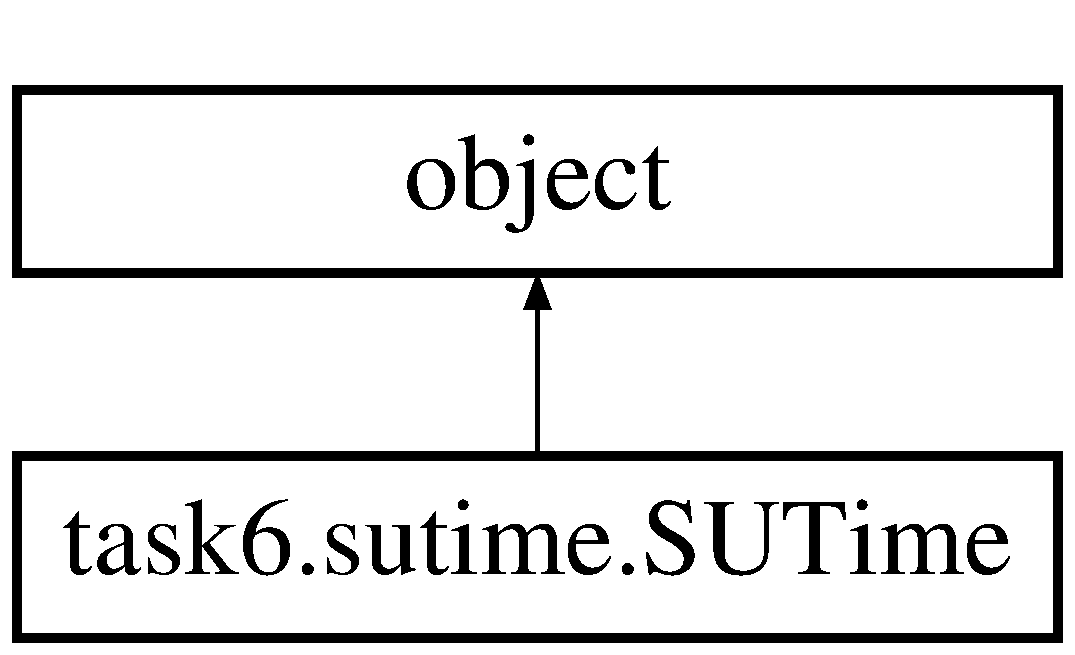
\includegraphics[height=2.000000cm]{classtask6_1_1sutime_1_1SUTime}
\end{center}
\end{figure}
\subsection*{Public Member Functions}
\begin{DoxyCompactItemize}
\item 
def \hyperlink{classtask6_1_1sutime_1_1SUTime_ad3d2f079441d91580b76c08e8cbbc01c}{\+\_\+\+\_\+init\+\_\+\+\_\+} (self, \hyperlink{classtask6_1_1sutime_1_1SUTime_aee86d05dd182246589b8f0eb6ea16897}{jars}=\mbox{[}$\,$\mbox{]}, jvm\+\_\+started=False, \hyperlink{classtask6_1_1sutime_1_1SUTime_a406b3a84a46ccab63a3b514e475d998e}{mark\+\_\+time\+\_\+ranges}=False, \hyperlink{classtask6_1_1sutime_1_1SUTime_a7e81771e26b1f92df6118f131798a034}{include\+\_\+range}=False)
\item 
def \hyperlink{classtask6_1_1sutime_1_1SUTime_a171448f34de8cab7d19e1353c8495c65}{parse} (self, input\+\_\+str, reference\+\_\+date=\textquotesingle{}\textquotesingle{})
\end{DoxyCompactItemize}
\subsection*{Public Attributes}
\begin{DoxyCompactItemize}
\item 
\hyperlink{classtask6_1_1sutime_1_1SUTime_a406b3a84a46ccab63a3b514e475d998e}{mark\+\_\+time\+\_\+ranges}
\item 
\hyperlink{classtask6_1_1sutime_1_1SUTime_a7e81771e26b1f92df6118f131798a034}{include\+\_\+range}
\item 
\hyperlink{classtask6_1_1sutime_1_1SUTime_aee86d05dd182246589b8f0eb6ea16897}{jars}
\end{DoxyCompactItemize}


\subsection{Detailed Description}
\begin{DoxyVerb}Python wrapper for SUTime (CoreNLP) by Stanford.

Attributes:
    jars: List of paths to the SUTime Java dependencies.
    jvm_started: Optional attribute to specify if the JVM has already been
        started (with all Java dependencies loaded).
    mark_time_ranges: Optional attribute to specify CoreNLP property
        sutime.markTimeRanges. Default is False.
        "Tells sutime to mark phrases such as 'From January to March'
        instead of marking 'January' and 'March' separately"
    include_range: Optional attribute to specify CoreNLP property
        sutime.includeRange. Default is False.
        "Tells sutime to mark phrases such as 'From January to March'
        instead of marking 'January' and 'March' separately"
\end{DoxyVerb}
 

Definition at line 11 of file sutime.\+py.



\subsection{Constructor \& Destructor Documentation}
\mbox{\Hypertarget{classtask6_1_1sutime_1_1SUTime_ad3d2f079441d91580b76c08e8cbbc01c}\label{classtask6_1_1sutime_1_1SUTime_ad3d2f079441d91580b76c08e8cbbc01c}} 
\index{task6\+::sutime\+::\+S\+U\+Time@{task6\+::sutime\+::\+S\+U\+Time}!\+\_\+\+\_\+init\+\_\+\+\_\+@{\+\_\+\+\_\+init\+\_\+\+\_\+}}
\index{\+\_\+\+\_\+init\+\_\+\+\_\+@{\+\_\+\+\_\+init\+\_\+\+\_\+}!task6\+::sutime\+::\+S\+U\+Time@{task6\+::sutime\+::\+S\+U\+Time}}
\subsubsection{\texorpdfstring{\+\_\+\+\_\+init\+\_\+\+\_\+()}{\_\_init\_\_()}}
{\footnotesize\ttfamily def task6.\+sutime.\+S\+U\+Time.\+\_\+\+\_\+init\+\_\+\+\_\+ (\begin{DoxyParamCaption}\item[{}]{self,  }\item[{}]{jars = {\ttfamily \mbox{[}\mbox{]}},  }\item[{}]{jvm\+\_\+started = {\ttfamily False},  }\item[{}]{mark\+\_\+time\+\_\+ranges = {\ttfamily False},  }\item[{}]{include\+\_\+range = {\ttfamily False} }\end{DoxyParamCaption})}

\begin{DoxyVerb}Initializes SUTime.
\end{DoxyVerb}
 

Definition at line 36 of file sutime.\+py.



\subsection{Member Function Documentation}
\mbox{\Hypertarget{classtask6_1_1sutime_1_1SUTime_a171448f34de8cab7d19e1353c8495c65}\label{classtask6_1_1sutime_1_1SUTime_a171448f34de8cab7d19e1353c8495c65}} 
\index{task6\+::sutime\+::\+S\+U\+Time@{task6\+::sutime\+::\+S\+U\+Time}!parse@{parse}}
\index{parse@{parse}!task6\+::sutime\+::\+S\+U\+Time@{task6\+::sutime\+::\+S\+U\+Time}}
\subsubsection{\texorpdfstring{parse()}{parse()}}
{\footnotesize\ttfamily def task6.\+sutime.\+S\+U\+Time.\+parse (\begin{DoxyParamCaption}\item[{}]{self,  }\item[{}]{input\+\_\+str,  }\item[{}]{reference\+\_\+date = {\ttfamily \textquotesingle{}\textquotesingle{}} }\end{DoxyParamCaption})}

\begin{DoxyVerb}Parses datetime information out of string input.

It invokes the SUTimeWrapper.annotate() function in Java.

Args:
    input_str: The input as string that has to be parsed.
    reference_date: Optional reference data for SUTime.

Returns:
    A list of dicts with the result from the SUTimeWrapper.annotate()
call.

Raises:
    RuntimeError: An error occurres when CoreNLP is not loaded.
\end{DoxyVerb}
 

Definition at line 95 of file sutime.\+py.



\subsection{Member Data Documentation}
\mbox{\Hypertarget{classtask6_1_1sutime_1_1SUTime_a7e81771e26b1f92df6118f131798a034}\label{classtask6_1_1sutime_1_1SUTime_a7e81771e26b1f92df6118f131798a034}} 
\index{task6\+::sutime\+::\+S\+U\+Time@{task6\+::sutime\+::\+S\+U\+Time}!include\+\_\+range@{include\+\_\+range}}
\index{include\+\_\+range@{include\+\_\+range}!task6\+::sutime\+::\+S\+U\+Time@{task6\+::sutime\+::\+S\+U\+Time}}
\subsubsection{\texorpdfstring{include\+\_\+range}{include\_range}}
{\footnotesize\ttfamily task6.\+sutime.\+S\+U\+Time.\+include\+\_\+range}



Definition at line 40 of file sutime.\+py.

\mbox{\Hypertarget{classtask6_1_1sutime_1_1SUTime_aee86d05dd182246589b8f0eb6ea16897}\label{classtask6_1_1sutime_1_1SUTime_aee86d05dd182246589b8f0eb6ea16897}} 
\index{task6\+::sutime\+::\+S\+U\+Time@{task6\+::sutime\+::\+S\+U\+Time}!jars@{jars}}
\index{jars@{jars}!task6\+::sutime\+::\+S\+U\+Time@{task6\+::sutime\+::\+S\+U\+Time}}
\subsubsection{\texorpdfstring{jars}{jars}}
{\footnotesize\ttfamily task6.\+sutime.\+S\+U\+Time.\+jars}



Definition at line 41 of file sutime.\+py.

\mbox{\Hypertarget{classtask6_1_1sutime_1_1SUTime_a406b3a84a46ccab63a3b514e475d998e}\label{classtask6_1_1sutime_1_1SUTime_a406b3a84a46ccab63a3b514e475d998e}} 
\index{task6\+::sutime\+::\+S\+U\+Time@{task6\+::sutime\+::\+S\+U\+Time}!mark\+\_\+time\+\_\+ranges@{mark\+\_\+time\+\_\+ranges}}
\index{mark\+\_\+time\+\_\+ranges@{mark\+\_\+time\+\_\+ranges}!task6\+::sutime\+::\+S\+U\+Time@{task6\+::sutime\+::\+S\+U\+Time}}
\subsubsection{\texorpdfstring{mark\+\_\+time\+\_\+ranges}{mark\_time\_ranges}}
{\footnotesize\ttfamily task6.\+sutime.\+S\+U\+Time.\+mark\+\_\+time\+\_\+ranges}



Definition at line 39 of file sutime.\+py.



The documentation for this class was generated from the following file\+:\begin{DoxyCompactItemize}
\item 
task6/\hyperlink{sutime_8py}{sutime.\+py}\end{DoxyCompactItemize}

\hypertarget{classtask6_1_1t6Entities_1_1T6AfterOperator}{}\section{task6.\+t6\+Entities.\+T6\+After\+Operator Class Reference}
\label{classtask6_1_1t6Entities_1_1T6AfterOperator}\index{task6.\+t6\+Entities.\+T6\+After\+Operator@{task6.\+t6\+Entities.\+T6\+After\+Operator}}
Inheritance diagram for task6.\+t6\+Entities.\+T6\+After\+Operator\+:\begin{figure}[H]
\begin{center}
\leavevmode
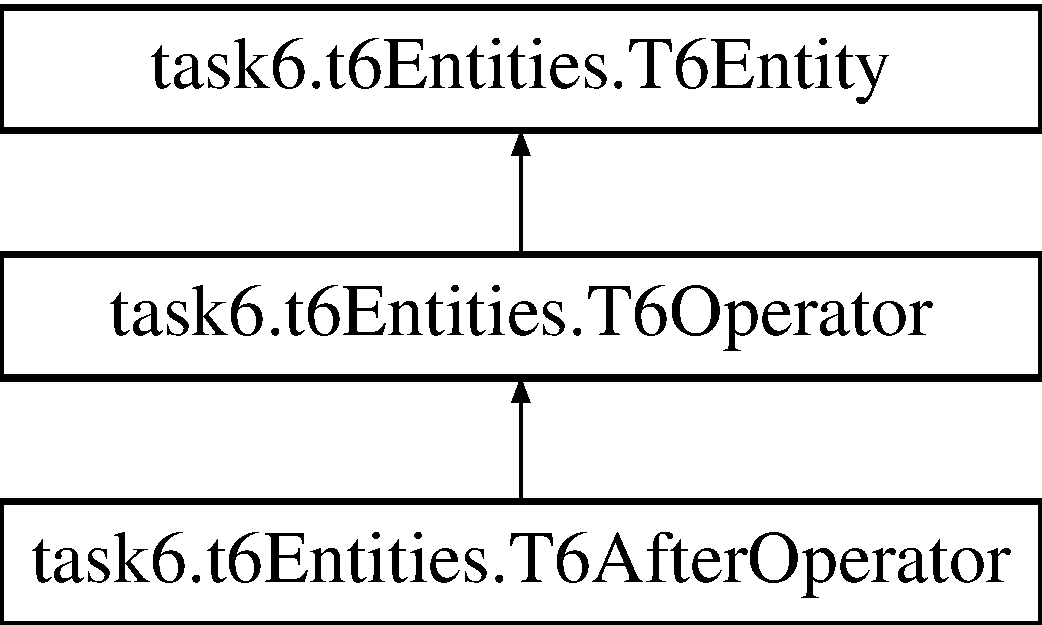
\includegraphics[height=3.000000cm]{classtask6_1_1t6Entities_1_1T6AfterOperator}
\end{center}
\end{figure}
\subsection*{Public Member Functions}
\begin{DoxyCompactItemize}
\item 
def \hyperlink{classtask6_1_1t6Entities_1_1T6AfterOperator_aec577149362a92ed1cf1e5bbdc0521c1}{\+\_\+\+\_\+init\+\_\+\+\_\+} (self, \hyperlink{classtask6_1_1t6Entities_1_1T6Entity_afeeced8134bb3ebe0cfecc64d0ab46a4}{id}, \hyperlink{classtask6_1_1t6Entities_1_1T6Entity_a52779e9af8864dc98e8b02fc5b9b041a}{start\+\_\+span}, \hyperlink{classtask6_1_1t6Entities_1_1T6Entity_aeb402200b156cd9562c5111dfe777b98}{end\+\_\+span}, \hyperlink{classtask6_1_1t6Entities_1_1T6AfterOperator_a4cecc35aaca42a517e7a8c3a23062b73}{interval\+\_\+type}, \hyperlink{classtask6_1_1t6Entities_1_1T6AfterOperator_a33c6453eb324ed64a62025d823329304}{interval}, \hyperlink{classtask6_1_1t6Entities_1_1T6AfterOperator_abb2b91e9891f20ec388cbc9d6038c3a7}{period}, \hyperlink{classtask6_1_1t6Entities_1_1T6AfterOperator_aa3611005a94f1cbc3867c3e3c9463d24}{repeating\+\_\+interval}, \hyperlink{classtask6_1_1t6Entities_1_1T6AfterOperator_a9a0d8b1907a272fa065b80fdd8a533a8}{semantics})
\end{DoxyCompactItemize}
\subsection*{Public Attributes}
\begin{DoxyCompactItemize}
\item 
\hyperlink{classtask6_1_1t6Entities_1_1T6AfterOperator_a4cecc35aaca42a517e7a8c3a23062b73}{interval\+\_\+type}
\item 
\hyperlink{classtask6_1_1t6Entities_1_1T6AfterOperator_a33c6453eb324ed64a62025d823329304}{interval}
\item 
\hyperlink{classtask6_1_1t6Entities_1_1T6AfterOperator_abb2b91e9891f20ec388cbc9d6038c3a7}{period}
\item 
\hyperlink{classtask6_1_1t6Entities_1_1T6AfterOperator_aa3611005a94f1cbc3867c3e3c9463d24}{repeating\+\_\+interval}
\item 
\hyperlink{classtask6_1_1t6Entities_1_1T6AfterOperator_a9a0d8b1907a272fa065b80fdd8a533a8}{semantics}
\end{DoxyCompactItemize}


\subsection{Detailed Description}


Definition at line 234 of file t6\+Entities.\+py.



\subsection{Constructor \& Destructor Documentation}
\mbox{\Hypertarget{classtask6_1_1t6Entities_1_1T6AfterOperator_aec577149362a92ed1cf1e5bbdc0521c1}\label{classtask6_1_1t6Entities_1_1T6AfterOperator_aec577149362a92ed1cf1e5bbdc0521c1}} 
\index{task6\+::t6\+Entities\+::\+T6\+After\+Operator@{task6\+::t6\+Entities\+::\+T6\+After\+Operator}!\+\_\+\+\_\+init\+\_\+\+\_\+@{\+\_\+\+\_\+init\+\_\+\+\_\+}}
\index{\+\_\+\+\_\+init\+\_\+\+\_\+@{\+\_\+\+\_\+init\+\_\+\+\_\+}!task6\+::t6\+Entities\+::\+T6\+After\+Operator@{task6\+::t6\+Entities\+::\+T6\+After\+Operator}}
\subsubsection{\texorpdfstring{\+\_\+\+\_\+init\+\_\+\+\_\+()}{\_\_init\_\_()}}
{\footnotesize\ttfamily def task6.\+t6\+Entities.\+T6\+After\+Operator.\+\_\+\+\_\+init\+\_\+\+\_\+ (\begin{DoxyParamCaption}\item[{}]{self,  }\item[{}]{id,  }\item[{}]{start\+\_\+span,  }\item[{}]{end\+\_\+span,  }\item[{}]{interval\+\_\+type,  }\item[{}]{interval,  }\item[{}]{period,  }\item[{}]{repeating\+\_\+interval,  }\item[{}]{semantics }\end{DoxyParamCaption})}



Definition at line 235 of file t6\+Entities.\+py.



\subsection{Member Data Documentation}
\mbox{\Hypertarget{classtask6_1_1t6Entities_1_1T6AfterOperator_a33c6453eb324ed64a62025d823329304}\label{classtask6_1_1t6Entities_1_1T6AfterOperator_a33c6453eb324ed64a62025d823329304}} 
\index{task6\+::t6\+Entities\+::\+T6\+After\+Operator@{task6\+::t6\+Entities\+::\+T6\+After\+Operator}!interval@{interval}}
\index{interval@{interval}!task6\+::t6\+Entities\+::\+T6\+After\+Operator@{task6\+::t6\+Entities\+::\+T6\+After\+Operator}}
\subsubsection{\texorpdfstring{interval}{interval}}
{\footnotesize\ttfamily task6.\+t6\+Entities.\+T6\+After\+Operator.\+interval}



Definition at line 238 of file t6\+Entities.\+py.

\mbox{\Hypertarget{classtask6_1_1t6Entities_1_1T6AfterOperator_a4cecc35aaca42a517e7a8c3a23062b73}\label{classtask6_1_1t6Entities_1_1T6AfterOperator_a4cecc35aaca42a517e7a8c3a23062b73}} 
\index{task6\+::t6\+Entities\+::\+T6\+After\+Operator@{task6\+::t6\+Entities\+::\+T6\+After\+Operator}!interval\+\_\+type@{interval\+\_\+type}}
\index{interval\+\_\+type@{interval\+\_\+type}!task6\+::t6\+Entities\+::\+T6\+After\+Operator@{task6\+::t6\+Entities\+::\+T6\+After\+Operator}}
\subsubsection{\texorpdfstring{interval\+\_\+type}{interval\_type}}
{\footnotesize\ttfamily task6.\+t6\+Entities.\+T6\+After\+Operator.\+interval\+\_\+type}



Definition at line 237 of file t6\+Entities.\+py.

\mbox{\Hypertarget{classtask6_1_1t6Entities_1_1T6AfterOperator_abb2b91e9891f20ec388cbc9d6038c3a7}\label{classtask6_1_1t6Entities_1_1T6AfterOperator_abb2b91e9891f20ec388cbc9d6038c3a7}} 
\index{task6\+::t6\+Entities\+::\+T6\+After\+Operator@{task6\+::t6\+Entities\+::\+T6\+After\+Operator}!period@{period}}
\index{period@{period}!task6\+::t6\+Entities\+::\+T6\+After\+Operator@{task6\+::t6\+Entities\+::\+T6\+After\+Operator}}
\subsubsection{\texorpdfstring{period}{period}}
{\footnotesize\ttfamily task6.\+t6\+Entities.\+T6\+After\+Operator.\+period}



Definition at line 239 of file t6\+Entities.\+py.

\mbox{\Hypertarget{classtask6_1_1t6Entities_1_1T6AfterOperator_aa3611005a94f1cbc3867c3e3c9463d24}\label{classtask6_1_1t6Entities_1_1T6AfterOperator_aa3611005a94f1cbc3867c3e3c9463d24}} 
\index{task6\+::t6\+Entities\+::\+T6\+After\+Operator@{task6\+::t6\+Entities\+::\+T6\+After\+Operator}!repeating\+\_\+interval@{repeating\+\_\+interval}}
\index{repeating\+\_\+interval@{repeating\+\_\+interval}!task6\+::t6\+Entities\+::\+T6\+After\+Operator@{task6\+::t6\+Entities\+::\+T6\+After\+Operator}}
\subsubsection{\texorpdfstring{repeating\+\_\+interval}{repeating\_interval}}
{\footnotesize\ttfamily task6.\+t6\+Entities.\+T6\+After\+Operator.\+repeating\+\_\+interval}



Definition at line 240 of file t6\+Entities.\+py.

\mbox{\Hypertarget{classtask6_1_1t6Entities_1_1T6AfterOperator_a9a0d8b1907a272fa065b80fdd8a533a8}\label{classtask6_1_1t6Entities_1_1T6AfterOperator_a9a0d8b1907a272fa065b80fdd8a533a8}} 
\index{task6\+::t6\+Entities\+::\+T6\+After\+Operator@{task6\+::t6\+Entities\+::\+T6\+After\+Operator}!semantics@{semantics}}
\index{semantics@{semantics}!task6\+::t6\+Entities\+::\+T6\+After\+Operator@{task6\+::t6\+Entities\+::\+T6\+After\+Operator}}
\subsubsection{\texorpdfstring{semantics}{semantics}}
{\footnotesize\ttfamily task6.\+t6\+Entities.\+T6\+After\+Operator.\+semantics}



Definition at line 241 of file t6\+Entities.\+py.



The documentation for this class was generated from the following file\+:\begin{DoxyCompactItemize}
\item 
task6/\hyperlink{t6Entities_8py}{t6\+Entities.\+py}\end{DoxyCompactItemize}

\hypertarget{classtask6_1_1t6Entities_1_1T6AMPMOfDay}{}\section{task6.\+t6\+Entities.\+T6\+A\+M\+P\+M\+Of\+Day Class Reference}
\label{classtask6_1_1t6Entities_1_1T6AMPMOfDay}\index{task6.\+t6\+Entities.\+T6\+A\+M\+P\+M\+Of\+Day@{task6.\+t6\+Entities.\+T6\+A\+M\+P\+M\+Of\+Day}}
Inheritance diagram for task6.\+t6\+Entities.\+T6\+A\+M\+P\+M\+Of\+Day\+:\begin{figure}[H]
\begin{center}
\leavevmode
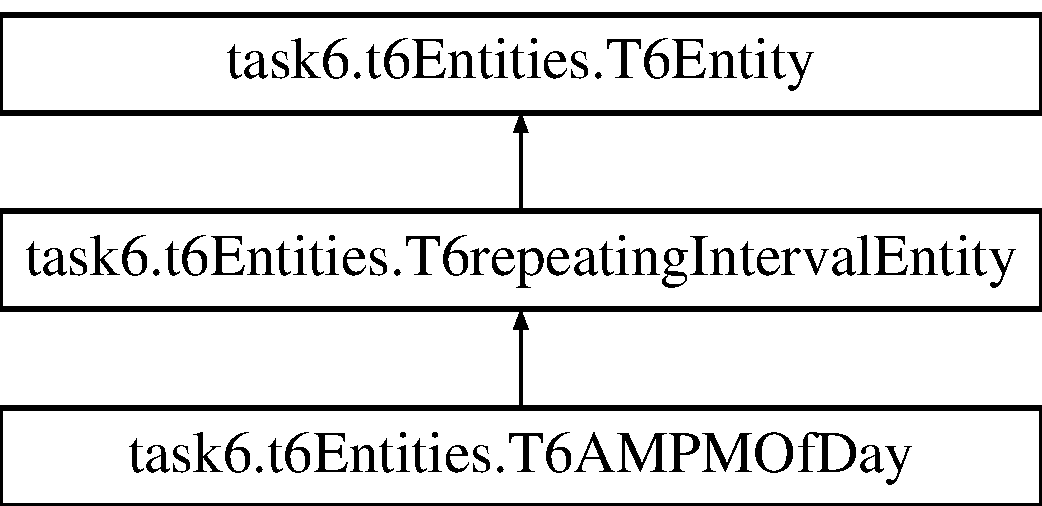
\includegraphics[height=3.000000cm]{classtask6_1_1t6Entities_1_1T6AMPMOfDay}
\end{center}
\end{figure}
\subsection*{Public Member Functions}
\begin{DoxyCompactItemize}
\item 
def \hyperlink{classtask6_1_1t6Entities_1_1T6AMPMOfDay_a800af0268e3964a5d98d53316c1d6fd4}{\+\_\+\+\_\+init\+\_\+\+\_\+} (self, \hyperlink{classtask6_1_1t6Entities_1_1T6Entity_afeeced8134bb3ebe0cfecc64d0ab46a4}{id}, \hyperlink{classtask6_1_1t6Entities_1_1T6Entity_a52779e9af8864dc98e8b02fc5b9b041a}{start\+\_\+span}, \hyperlink{classtask6_1_1t6Entities_1_1T6Entity_aeb402200b156cd9562c5111dfe777b98}{end\+\_\+span}, \hyperlink{classtask6_1_1t6Entities_1_1T6AMPMOfDay_ad5d347e7a4819e052b39c4709d08038d}{ampm\+\_\+type}, \hyperlink{classtask6_1_1t6Entities_1_1T6AMPMOfDay_a3d94781e4fb82b58d2adc8637bf515ac}{number}, \hyperlink{classtask6_1_1t6Entities_1_1T6AMPMOfDay_a775ca0b3161fef5d092cd5364bc4a954}{modifier})
\end{DoxyCompactItemize}
\subsection*{Public Attributes}
\begin{DoxyCompactItemize}
\item 
\hyperlink{classtask6_1_1t6Entities_1_1T6AMPMOfDay_ad5d347e7a4819e052b39c4709d08038d}{ampm\+\_\+type}
\item 
\hyperlink{classtask6_1_1t6Entities_1_1T6AMPMOfDay_a3d94781e4fb82b58d2adc8637bf515ac}{number}
\item 
\hyperlink{classtask6_1_1t6Entities_1_1T6AMPMOfDay_a775ca0b3161fef5d092cd5364bc4a954}{modifier}
\end{DoxyCompactItemize}


\subsection{Detailed Description}


Definition at line 156 of file t6\+Entities.\+py.



\subsection{Constructor \& Destructor Documentation}
\mbox{\Hypertarget{classtask6_1_1t6Entities_1_1T6AMPMOfDay_a800af0268e3964a5d98d53316c1d6fd4}\label{classtask6_1_1t6Entities_1_1T6AMPMOfDay_a800af0268e3964a5d98d53316c1d6fd4}} 
\index{task6\+::t6\+Entities\+::\+T6\+A\+M\+P\+M\+Of\+Day@{task6\+::t6\+Entities\+::\+T6\+A\+M\+P\+M\+Of\+Day}!\+\_\+\+\_\+init\+\_\+\+\_\+@{\+\_\+\+\_\+init\+\_\+\+\_\+}}
\index{\+\_\+\+\_\+init\+\_\+\+\_\+@{\+\_\+\+\_\+init\+\_\+\+\_\+}!task6\+::t6\+Entities\+::\+T6\+A\+M\+P\+M\+Of\+Day@{task6\+::t6\+Entities\+::\+T6\+A\+M\+P\+M\+Of\+Day}}
\subsubsection{\texorpdfstring{\+\_\+\+\_\+init\+\_\+\+\_\+()}{\_\_init\_\_()}}
{\footnotesize\ttfamily def task6.\+t6\+Entities.\+T6\+A\+M\+P\+M\+Of\+Day.\+\_\+\+\_\+init\+\_\+\+\_\+ (\begin{DoxyParamCaption}\item[{}]{self,  }\item[{}]{id,  }\item[{}]{start\+\_\+span,  }\item[{}]{end\+\_\+span,  }\item[{}]{ampm\+\_\+type,  }\item[{}]{number,  }\item[{}]{modifier }\end{DoxyParamCaption})}



Definition at line 157 of file t6\+Entities.\+py.



\subsection{Member Data Documentation}
\mbox{\Hypertarget{classtask6_1_1t6Entities_1_1T6AMPMOfDay_ad5d347e7a4819e052b39c4709d08038d}\label{classtask6_1_1t6Entities_1_1T6AMPMOfDay_ad5d347e7a4819e052b39c4709d08038d}} 
\index{task6\+::t6\+Entities\+::\+T6\+A\+M\+P\+M\+Of\+Day@{task6\+::t6\+Entities\+::\+T6\+A\+M\+P\+M\+Of\+Day}!ampm\+\_\+type@{ampm\+\_\+type}}
\index{ampm\+\_\+type@{ampm\+\_\+type}!task6\+::t6\+Entities\+::\+T6\+A\+M\+P\+M\+Of\+Day@{task6\+::t6\+Entities\+::\+T6\+A\+M\+P\+M\+Of\+Day}}
\subsubsection{\texorpdfstring{ampm\+\_\+type}{ampm\_type}}
{\footnotesize\ttfamily task6.\+t6\+Entities.\+T6\+A\+M\+P\+M\+Of\+Day.\+ampm\+\_\+type}



Definition at line 159 of file t6\+Entities.\+py.

\mbox{\Hypertarget{classtask6_1_1t6Entities_1_1T6AMPMOfDay_a775ca0b3161fef5d092cd5364bc4a954}\label{classtask6_1_1t6Entities_1_1T6AMPMOfDay_a775ca0b3161fef5d092cd5364bc4a954}} 
\index{task6\+::t6\+Entities\+::\+T6\+A\+M\+P\+M\+Of\+Day@{task6\+::t6\+Entities\+::\+T6\+A\+M\+P\+M\+Of\+Day}!modifier@{modifier}}
\index{modifier@{modifier}!task6\+::t6\+Entities\+::\+T6\+A\+M\+P\+M\+Of\+Day@{task6\+::t6\+Entities\+::\+T6\+A\+M\+P\+M\+Of\+Day}}
\subsubsection{\texorpdfstring{modifier}{modifier}}
{\footnotesize\ttfamily task6.\+t6\+Entities.\+T6\+A\+M\+P\+M\+Of\+Day.\+modifier}



Definition at line 161 of file t6\+Entities.\+py.

\mbox{\Hypertarget{classtask6_1_1t6Entities_1_1T6AMPMOfDay_a3d94781e4fb82b58d2adc8637bf515ac}\label{classtask6_1_1t6Entities_1_1T6AMPMOfDay_a3d94781e4fb82b58d2adc8637bf515ac}} 
\index{task6\+::t6\+Entities\+::\+T6\+A\+M\+P\+M\+Of\+Day@{task6\+::t6\+Entities\+::\+T6\+A\+M\+P\+M\+Of\+Day}!number@{number}}
\index{number@{number}!task6\+::t6\+Entities\+::\+T6\+A\+M\+P\+M\+Of\+Day@{task6\+::t6\+Entities\+::\+T6\+A\+M\+P\+M\+Of\+Day}}
\subsubsection{\texorpdfstring{number}{number}}
{\footnotesize\ttfamily task6.\+t6\+Entities.\+T6\+A\+M\+P\+M\+Of\+Day.\+number}



Definition at line 160 of file t6\+Entities.\+py.



The documentation for this class was generated from the following file\+:\begin{DoxyCompactItemize}
\item 
task6/\hyperlink{t6Entities_8py}{t6\+Entities.\+py}\end{DoxyCompactItemize}

\hypertarget{classtask6_1_1t6Entities_1_1T6BeforeOperator}{}\section{task6.\+t6\+Entities.\+T6\+Before\+Operator Class Reference}
\label{classtask6_1_1t6Entities_1_1T6BeforeOperator}\index{task6.\+t6\+Entities.\+T6\+Before\+Operator@{task6.\+t6\+Entities.\+T6\+Before\+Operator}}
Inheritance diagram for task6.\+t6\+Entities.\+T6\+Before\+Operator\+:\begin{figure}[H]
\begin{center}
\leavevmode
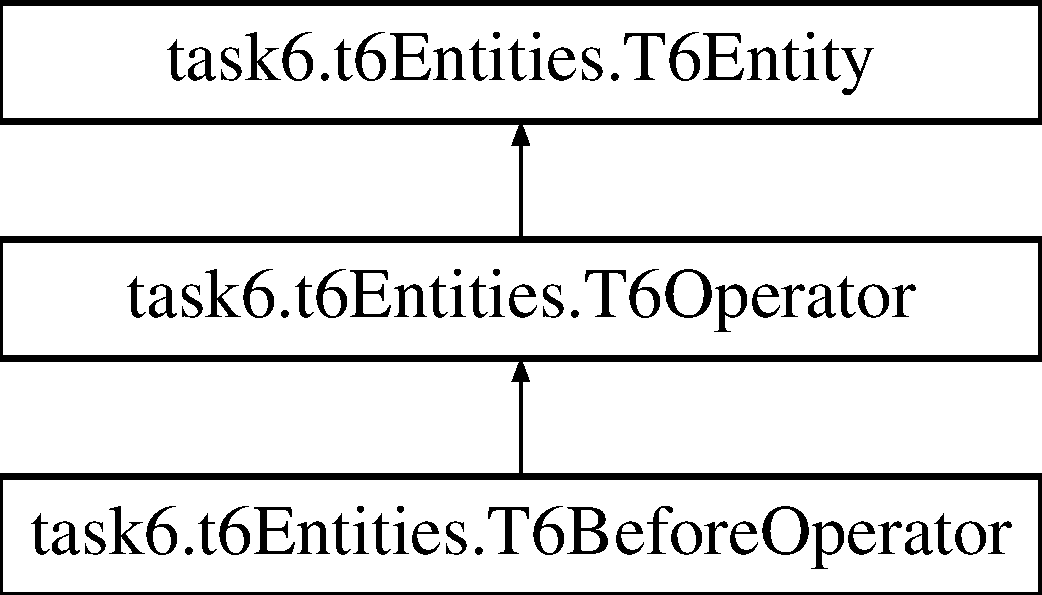
\includegraphics[height=3.000000cm]{classtask6_1_1t6Entities_1_1T6BeforeOperator}
\end{center}
\end{figure}
\subsection*{Public Member Functions}
\begin{DoxyCompactItemize}
\item 
def \hyperlink{classtask6_1_1t6Entities_1_1T6BeforeOperator_a2a546c7ff84c52a10018e1cab9a59ef2}{\+\_\+\+\_\+init\+\_\+\+\_\+} (self, \hyperlink{classtask6_1_1t6Entities_1_1T6Entity_afeeced8134bb3ebe0cfecc64d0ab46a4}{id}, \hyperlink{classtask6_1_1t6Entities_1_1T6Entity_a52779e9af8864dc98e8b02fc5b9b041a}{start\+\_\+span}, \hyperlink{classtask6_1_1t6Entities_1_1T6Entity_aeb402200b156cd9562c5111dfe777b98}{end\+\_\+span}, \hyperlink{classtask6_1_1t6Entities_1_1T6BeforeOperator_a21cf9f8f978c26b5a2f70808a38d3cbf}{interval\+\_\+type}, \hyperlink{classtask6_1_1t6Entities_1_1T6BeforeOperator_ae1949d02c8d0ec34aa880a7c2165b69b}{interval}, \hyperlink{classtask6_1_1t6Entities_1_1T6BeforeOperator_a5d08ebe378bdb8b689cf2bf65a093f7e}{period}, \hyperlink{classtask6_1_1t6Entities_1_1T6BeforeOperator_a07e3c77e0df7c9afe548326b004b569b}{repeating\+\_\+interval})
\end{DoxyCompactItemize}
\subsection*{Public Attributes}
\begin{DoxyCompactItemize}
\item 
\hyperlink{classtask6_1_1t6Entities_1_1T6BeforeOperator_a21cf9f8f978c26b5a2f70808a38d3cbf}{interval\+\_\+type}
\item 
\hyperlink{classtask6_1_1t6Entities_1_1T6BeforeOperator_ae1949d02c8d0ec34aa880a7c2165b69b}{interval}
\item 
\hyperlink{classtask6_1_1t6Entities_1_1T6BeforeOperator_a5d08ebe378bdb8b689cf2bf65a093f7e}{period}
\item 
\hyperlink{classtask6_1_1t6Entities_1_1T6BeforeOperator_a07e3c77e0df7c9afe548326b004b569b}{repeating\+\_\+interval}
\end{DoxyCompactItemize}


\subsection{Detailed Description}


Definition at line 226 of file t6\+Entities.\+py.



\subsection{Constructor \& Destructor Documentation}
\mbox{\Hypertarget{classtask6_1_1t6Entities_1_1T6BeforeOperator_a2a546c7ff84c52a10018e1cab9a59ef2}\label{classtask6_1_1t6Entities_1_1T6BeforeOperator_a2a546c7ff84c52a10018e1cab9a59ef2}} 
\index{task6\+::t6\+Entities\+::\+T6\+Before\+Operator@{task6\+::t6\+Entities\+::\+T6\+Before\+Operator}!\+\_\+\+\_\+init\+\_\+\+\_\+@{\+\_\+\+\_\+init\+\_\+\+\_\+}}
\index{\+\_\+\+\_\+init\+\_\+\+\_\+@{\+\_\+\+\_\+init\+\_\+\+\_\+}!task6\+::t6\+Entities\+::\+T6\+Before\+Operator@{task6\+::t6\+Entities\+::\+T6\+Before\+Operator}}
\subsubsection{\texorpdfstring{\+\_\+\+\_\+init\+\_\+\+\_\+()}{\_\_init\_\_()}}
{\footnotesize\ttfamily def task6.\+t6\+Entities.\+T6\+Before\+Operator.\+\_\+\+\_\+init\+\_\+\+\_\+ (\begin{DoxyParamCaption}\item[{}]{self,  }\item[{}]{id,  }\item[{}]{start\+\_\+span,  }\item[{}]{end\+\_\+span,  }\item[{}]{interval\+\_\+type,  }\item[{}]{interval,  }\item[{}]{period,  }\item[{}]{repeating\+\_\+interval }\end{DoxyParamCaption})}



Definition at line 227 of file t6\+Entities.\+py.



\subsection{Member Data Documentation}
\mbox{\Hypertarget{classtask6_1_1t6Entities_1_1T6BeforeOperator_ae1949d02c8d0ec34aa880a7c2165b69b}\label{classtask6_1_1t6Entities_1_1T6BeforeOperator_ae1949d02c8d0ec34aa880a7c2165b69b}} 
\index{task6\+::t6\+Entities\+::\+T6\+Before\+Operator@{task6\+::t6\+Entities\+::\+T6\+Before\+Operator}!interval@{interval}}
\index{interval@{interval}!task6\+::t6\+Entities\+::\+T6\+Before\+Operator@{task6\+::t6\+Entities\+::\+T6\+Before\+Operator}}
\subsubsection{\texorpdfstring{interval}{interval}}
{\footnotesize\ttfamily task6.\+t6\+Entities.\+T6\+Before\+Operator.\+interval}



Definition at line 230 of file t6\+Entities.\+py.

\mbox{\Hypertarget{classtask6_1_1t6Entities_1_1T6BeforeOperator_a21cf9f8f978c26b5a2f70808a38d3cbf}\label{classtask6_1_1t6Entities_1_1T6BeforeOperator_a21cf9f8f978c26b5a2f70808a38d3cbf}} 
\index{task6\+::t6\+Entities\+::\+T6\+Before\+Operator@{task6\+::t6\+Entities\+::\+T6\+Before\+Operator}!interval\+\_\+type@{interval\+\_\+type}}
\index{interval\+\_\+type@{interval\+\_\+type}!task6\+::t6\+Entities\+::\+T6\+Before\+Operator@{task6\+::t6\+Entities\+::\+T6\+Before\+Operator}}
\subsubsection{\texorpdfstring{interval\+\_\+type}{interval\_type}}
{\footnotesize\ttfamily task6.\+t6\+Entities.\+T6\+Before\+Operator.\+interval\+\_\+type}



Definition at line 229 of file t6\+Entities.\+py.

\mbox{\Hypertarget{classtask6_1_1t6Entities_1_1T6BeforeOperator_a5d08ebe378bdb8b689cf2bf65a093f7e}\label{classtask6_1_1t6Entities_1_1T6BeforeOperator_a5d08ebe378bdb8b689cf2bf65a093f7e}} 
\index{task6\+::t6\+Entities\+::\+T6\+Before\+Operator@{task6\+::t6\+Entities\+::\+T6\+Before\+Operator}!period@{period}}
\index{period@{period}!task6\+::t6\+Entities\+::\+T6\+Before\+Operator@{task6\+::t6\+Entities\+::\+T6\+Before\+Operator}}
\subsubsection{\texorpdfstring{period}{period}}
{\footnotesize\ttfamily task6.\+t6\+Entities.\+T6\+Before\+Operator.\+period}



Definition at line 231 of file t6\+Entities.\+py.

\mbox{\Hypertarget{classtask6_1_1t6Entities_1_1T6BeforeOperator_a07e3c77e0df7c9afe548326b004b569b}\label{classtask6_1_1t6Entities_1_1T6BeforeOperator_a07e3c77e0df7c9afe548326b004b569b}} 
\index{task6\+::t6\+Entities\+::\+T6\+Before\+Operator@{task6\+::t6\+Entities\+::\+T6\+Before\+Operator}!repeating\+\_\+interval@{repeating\+\_\+interval}}
\index{repeating\+\_\+interval@{repeating\+\_\+interval}!task6\+::t6\+Entities\+::\+T6\+Before\+Operator@{task6\+::t6\+Entities\+::\+T6\+Before\+Operator}}
\subsubsection{\texorpdfstring{repeating\+\_\+interval}{repeating\_interval}}
{\footnotesize\ttfamily task6.\+t6\+Entities.\+T6\+Before\+Operator.\+repeating\+\_\+interval}



Definition at line 232 of file t6\+Entities.\+py.



The documentation for this class was generated from the following file\+:\begin{DoxyCompactItemize}
\item 
task6/\hyperlink{t6Entities_8py}{t6\+Entities.\+py}\end{DoxyCompactItemize}

\hypertarget{classtask6_1_1t6Entities_1_1T6BetweenOperator}{}\section{task6.\+t6\+Entities.\+T6\+Between\+Operator Class Reference}
\label{classtask6_1_1t6Entities_1_1T6BetweenOperator}\index{task6.\+t6\+Entities.\+T6\+Between\+Operator@{task6.\+t6\+Entities.\+T6\+Between\+Operator}}
Inheritance diagram for task6.\+t6\+Entities.\+T6\+Between\+Operator\+:\begin{figure}[H]
\begin{center}
\leavevmode
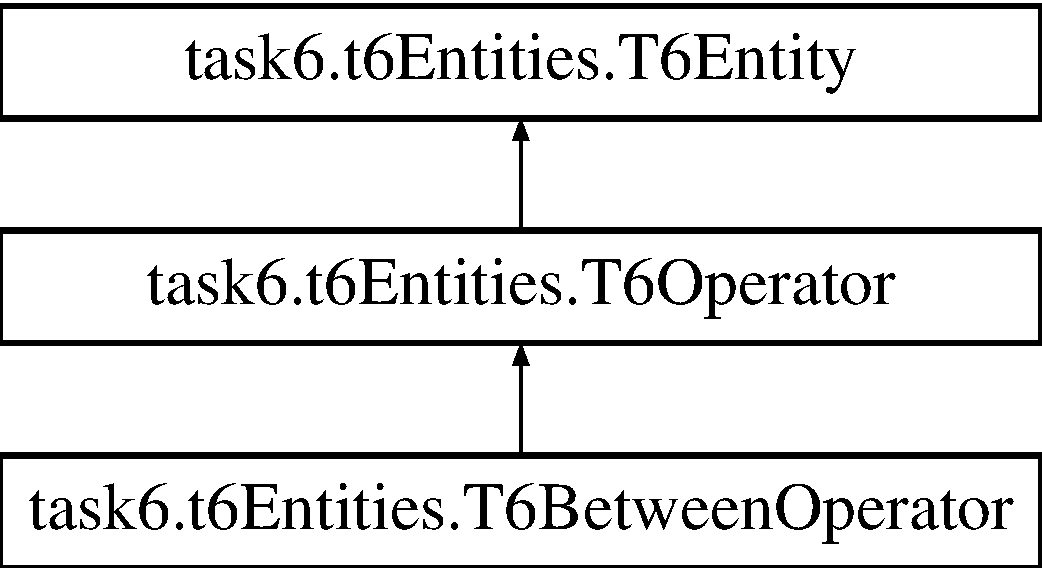
\includegraphics[height=3.000000cm]{classtask6_1_1t6Entities_1_1T6BetweenOperator}
\end{center}
\end{figure}
\subsection*{Public Member Functions}
\begin{DoxyCompactItemize}
\item 
def \hyperlink{classtask6_1_1t6Entities_1_1T6BetweenOperator_a5f14461e7680898e99d0ffae4e7cabf3}{\+\_\+\+\_\+init\+\_\+\+\_\+} (self, \hyperlink{classtask6_1_1t6Entities_1_1T6Entity_afeeced8134bb3ebe0cfecc64d0ab46a4}{id}, \hyperlink{classtask6_1_1t6Entities_1_1T6Entity_a52779e9af8864dc98e8b02fc5b9b041a}{start\+\_\+span}, \hyperlink{classtask6_1_1t6Entities_1_1T6Entity_aeb402200b156cd9562c5111dfe777b98}{end\+\_\+span}, \hyperlink{classtask6_1_1t6Entities_1_1T6BetweenOperator_a35cf4635c9e2556637c8943ef997c1f5}{interval\+\_\+type}, \hyperlink{classtask6_1_1t6Entities_1_1T6BetweenOperator_a9eb5c4526dd584bd2390d9b864098869}{interval}, \hyperlink{classtask6_1_1t6Entities_1_1T6BetweenOperator_a764d758517da34169e3b313f7d6a2789}{period}, \hyperlink{classtask6_1_1t6Entities_1_1T6BetweenOperator_a43793dba1ed7f6ee2c940f79559d5eaf}{repeating\+\_\+interval})
\end{DoxyCompactItemize}
\subsection*{Public Attributes}
\begin{DoxyCompactItemize}
\item 
\hyperlink{classtask6_1_1t6Entities_1_1T6BetweenOperator_a35cf4635c9e2556637c8943ef997c1f5}{interval\+\_\+type}
\item 
\hyperlink{classtask6_1_1t6Entities_1_1T6BetweenOperator_a9eb5c4526dd584bd2390d9b864098869}{interval}
\item 
\hyperlink{classtask6_1_1t6Entities_1_1T6BetweenOperator_a764d758517da34169e3b313f7d6a2789}{period}
\item 
\hyperlink{classtask6_1_1t6Entities_1_1T6BetweenOperator_a43793dba1ed7f6ee2c940f79559d5eaf}{repeating\+\_\+interval}
\end{DoxyCompactItemize}


\subsection{Detailed Description}


Definition at line 243 of file t6\+Entities.\+py.



\subsection{Constructor \& Destructor Documentation}
\mbox{\Hypertarget{classtask6_1_1t6Entities_1_1T6BetweenOperator_a5f14461e7680898e99d0ffae4e7cabf3}\label{classtask6_1_1t6Entities_1_1T6BetweenOperator_a5f14461e7680898e99d0ffae4e7cabf3}} 
\index{task6\+::t6\+Entities\+::\+T6\+Between\+Operator@{task6\+::t6\+Entities\+::\+T6\+Between\+Operator}!\+\_\+\+\_\+init\+\_\+\+\_\+@{\+\_\+\+\_\+init\+\_\+\+\_\+}}
\index{\+\_\+\+\_\+init\+\_\+\+\_\+@{\+\_\+\+\_\+init\+\_\+\+\_\+}!task6\+::t6\+Entities\+::\+T6\+Between\+Operator@{task6\+::t6\+Entities\+::\+T6\+Between\+Operator}}
\subsubsection{\texorpdfstring{\+\_\+\+\_\+init\+\_\+\+\_\+()}{\_\_init\_\_()}}
{\footnotesize\ttfamily def task6.\+t6\+Entities.\+T6\+Between\+Operator.\+\_\+\+\_\+init\+\_\+\+\_\+ (\begin{DoxyParamCaption}\item[{}]{self,  }\item[{}]{id,  }\item[{}]{start\+\_\+span,  }\item[{}]{end\+\_\+span,  }\item[{}]{interval\+\_\+type,  }\item[{}]{interval,  }\item[{}]{period,  }\item[{}]{repeating\+\_\+interval }\end{DoxyParamCaption})}



Definition at line 244 of file t6\+Entities.\+py.



\subsection{Member Data Documentation}
\mbox{\Hypertarget{classtask6_1_1t6Entities_1_1T6BetweenOperator_a9eb5c4526dd584bd2390d9b864098869}\label{classtask6_1_1t6Entities_1_1T6BetweenOperator_a9eb5c4526dd584bd2390d9b864098869}} 
\index{task6\+::t6\+Entities\+::\+T6\+Between\+Operator@{task6\+::t6\+Entities\+::\+T6\+Between\+Operator}!interval@{interval}}
\index{interval@{interval}!task6\+::t6\+Entities\+::\+T6\+Between\+Operator@{task6\+::t6\+Entities\+::\+T6\+Between\+Operator}}
\subsubsection{\texorpdfstring{interval}{interval}}
{\footnotesize\ttfamily task6.\+t6\+Entities.\+T6\+Between\+Operator.\+interval}



Definition at line 247 of file t6\+Entities.\+py.

\mbox{\Hypertarget{classtask6_1_1t6Entities_1_1T6BetweenOperator_a35cf4635c9e2556637c8943ef997c1f5}\label{classtask6_1_1t6Entities_1_1T6BetweenOperator_a35cf4635c9e2556637c8943ef997c1f5}} 
\index{task6\+::t6\+Entities\+::\+T6\+Between\+Operator@{task6\+::t6\+Entities\+::\+T6\+Between\+Operator}!interval\+\_\+type@{interval\+\_\+type}}
\index{interval\+\_\+type@{interval\+\_\+type}!task6\+::t6\+Entities\+::\+T6\+Between\+Operator@{task6\+::t6\+Entities\+::\+T6\+Between\+Operator}}
\subsubsection{\texorpdfstring{interval\+\_\+type}{interval\_type}}
{\footnotesize\ttfamily task6.\+t6\+Entities.\+T6\+Between\+Operator.\+interval\+\_\+type}



Definition at line 246 of file t6\+Entities.\+py.

\mbox{\Hypertarget{classtask6_1_1t6Entities_1_1T6BetweenOperator_a764d758517da34169e3b313f7d6a2789}\label{classtask6_1_1t6Entities_1_1T6BetweenOperator_a764d758517da34169e3b313f7d6a2789}} 
\index{task6\+::t6\+Entities\+::\+T6\+Between\+Operator@{task6\+::t6\+Entities\+::\+T6\+Between\+Operator}!period@{period}}
\index{period@{period}!task6\+::t6\+Entities\+::\+T6\+Between\+Operator@{task6\+::t6\+Entities\+::\+T6\+Between\+Operator}}
\subsubsection{\texorpdfstring{period}{period}}
{\footnotesize\ttfamily task6.\+t6\+Entities.\+T6\+Between\+Operator.\+period}



Definition at line 248 of file t6\+Entities.\+py.

\mbox{\Hypertarget{classtask6_1_1t6Entities_1_1T6BetweenOperator_a43793dba1ed7f6ee2c940f79559d5eaf}\label{classtask6_1_1t6Entities_1_1T6BetweenOperator_a43793dba1ed7f6ee2c940f79559d5eaf}} 
\index{task6\+::t6\+Entities\+::\+T6\+Between\+Operator@{task6\+::t6\+Entities\+::\+T6\+Between\+Operator}!repeating\+\_\+interval@{repeating\+\_\+interval}}
\index{repeating\+\_\+interval@{repeating\+\_\+interval}!task6\+::t6\+Entities\+::\+T6\+Between\+Operator@{task6\+::t6\+Entities\+::\+T6\+Between\+Operator}}
\subsubsection{\texorpdfstring{repeating\+\_\+interval}{repeating\_interval}}
{\footnotesize\ttfamily task6.\+t6\+Entities.\+T6\+Between\+Operator.\+repeating\+\_\+interval}



Definition at line 249 of file t6\+Entities.\+py.



The documentation for this class was generated from the following file\+:\begin{DoxyCompactItemize}
\item 
task6/\hyperlink{t6Entities_8py}{t6\+Entities.\+py}\end{DoxyCompactItemize}

\hypertarget{classtask6_1_1t6Entities_1_1T6CalendarIntervalEntity}{}\section{task6.\+t6\+Entities.\+T6\+Calendar\+Interval\+Entity Class Reference}
\label{classtask6_1_1t6Entities_1_1T6CalendarIntervalEntity}\index{task6.\+t6\+Entities.\+T6\+Calendar\+Interval\+Entity@{task6.\+t6\+Entities.\+T6\+Calendar\+Interval\+Entity}}
Inheritance diagram for task6.\+t6\+Entities.\+T6\+Calendar\+Interval\+Entity\+:\begin{figure}[H]
\begin{center}
\leavevmode
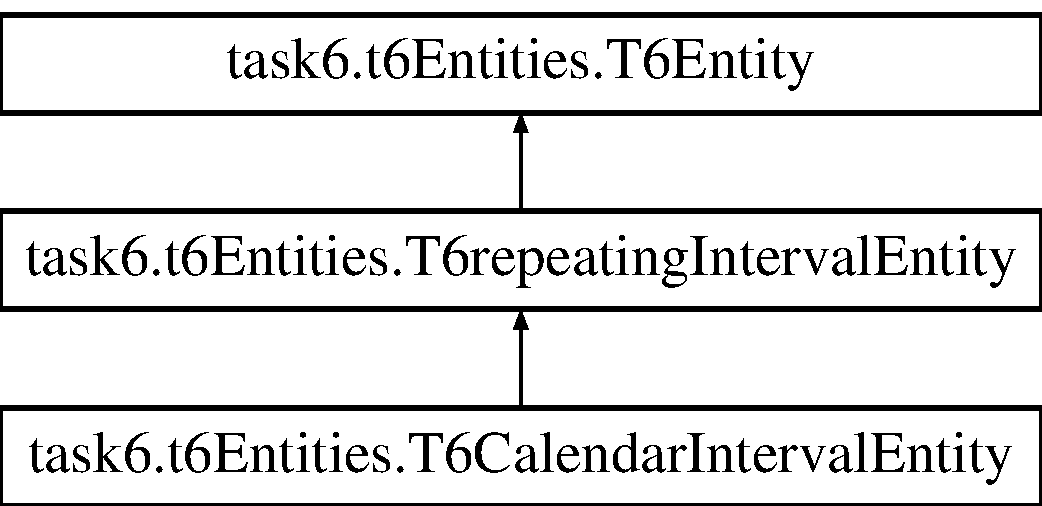
\includegraphics[height=3.000000cm]{classtask6_1_1t6Entities_1_1T6CalendarIntervalEntity}
\end{center}
\end{figure}
\subsection*{Public Member Functions}
\begin{DoxyCompactItemize}
\item 
def \hyperlink{classtask6_1_1t6Entities_1_1T6CalendarIntervalEntity_a5cbe4f08ae498af3f13edbd42e8d02d3}{\+\_\+\+\_\+init\+\_\+\+\_\+} (self, \hyperlink{classtask6_1_1t6Entities_1_1T6Entity_afeeced8134bb3ebe0cfecc64d0ab46a4}{id}, \hyperlink{classtask6_1_1t6Entities_1_1T6Entity_a52779e9af8864dc98e8b02fc5b9b041a}{start\+\_\+span}, \hyperlink{classtask6_1_1t6Entities_1_1T6Entity_aeb402200b156cd9562c5111dfe777b98}{end\+\_\+span}, \hyperlink{classtask6_1_1t6Entities_1_1T6CalendarIntervalEntity_a57d20d358dfc92c6b25f04c2296ee919}{calendar\+\_\+type}, \hyperlink{classtask6_1_1t6Entities_1_1T6CalendarIntervalEntity_acfb01d089dbc4f2fe2e433c74405b950}{number}, \hyperlink{classtask6_1_1t6Entities_1_1T6CalendarIntervalEntity_ae40ab2003ae494a5e478e7614f26acd9}{modifier})
\end{DoxyCompactItemize}
\subsection*{Public Attributes}
\begin{DoxyCompactItemize}
\item 
\hyperlink{classtask6_1_1t6Entities_1_1T6CalendarIntervalEntity_a57d20d358dfc92c6b25f04c2296ee919}{calendar\+\_\+type}
\item 
\hyperlink{classtask6_1_1t6Entities_1_1T6CalendarIntervalEntity_acfb01d089dbc4f2fe2e433c74405b950}{number}
\item 
\hyperlink{classtask6_1_1t6Entities_1_1T6CalendarIntervalEntity_ae40ab2003ae494a5e478e7614f26acd9}{modifier}
\end{DoxyCompactItemize}


\subsection{Detailed Description}


Definition at line 142 of file t6\+Entities.\+py.



\subsection{Constructor \& Destructor Documentation}
\mbox{\Hypertarget{classtask6_1_1t6Entities_1_1T6CalendarIntervalEntity_a5cbe4f08ae498af3f13edbd42e8d02d3}\label{classtask6_1_1t6Entities_1_1T6CalendarIntervalEntity_a5cbe4f08ae498af3f13edbd42e8d02d3}} 
\index{task6\+::t6\+Entities\+::\+T6\+Calendar\+Interval\+Entity@{task6\+::t6\+Entities\+::\+T6\+Calendar\+Interval\+Entity}!\+\_\+\+\_\+init\+\_\+\+\_\+@{\+\_\+\+\_\+init\+\_\+\+\_\+}}
\index{\+\_\+\+\_\+init\+\_\+\+\_\+@{\+\_\+\+\_\+init\+\_\+\+\_\+}!task6\+::t6\+Entities\+::\+T6\+Calendar\+Interval\+Entity@{task6\+::t6\+Entities\+::\+T6\+Calendar\+Interval\+Entity}}
\subsubsection{\texorpdfstring{\+\_\+\+\_\+init\+\_\+\+\_\+()}{\_\_init\_\_()}}
{\footnotesize\ttfamily def task6.\+t6\+Entities.\+T6\+Calendar\+Interval\+Entity.\+\_\+\+\_\+init\+\_\+\+\_\+ (\begin{DoxyParamCaption}\item[{}]{self,  }\item[{}]{id,  }\item[{}]{start\+\_\+span,  }\item[{}]{end\+\_\+span,  }\item[{}]{calendar\+\_\+type,  }\item[{}]{number,  }\item[{}]{modifier }\end{DoxyParamCaption})}



Definition at line 143 of file t6\+Entities.\+py.



\subsection{Member Data Documentation}
\mbox{\Hypertarget{classtask6_1_1t6Entities_1_1T6CalendarIntervalEntity_a57d20d358dfc92c6b25f04c2296ee919}\label{classtask6_1_1t6Entities_1_1T6CalendarIntervalEntity_a57d20d358dfc92c6b25f04c2296ee919}} 
\index{task6\+::t6\+Entities\+::\+T6\+Calendar\+Interval\+Entity@{task6\+::t6\+Entities\+::\+T6\+Calendar\+Interval\+Entity}!calendar\+\_\+type@{calendar\+\_\+type}}
\index{calendar\+\_\+type@{calendar\+\_\+type}!task6\+::t6\+Entities\+::\+T6\+Calendar\+Interval\+Entity@{task6\+::t6\+Entities\+::\+T6\+Calendar\+Interval\+Entity}}
\subsubsection{\texorpdfstring{calendar\+\_\+type}{calendar\_type}}
{\footnotesize\ttfamily task6.\+t6\+Entities.\+T6\+Calendar\+Interval\+Entity.\+calendar\+\_\+type}



Definition at line 145 of file t6\+Entities.\+py.

\mbox{\Hypertarget{classtask6_1_1t6Entities_1_1T6CalendarIntervalEntity_ae40ab2003ae494a5e478e7614f26acd9}\label{classtask6_1_1t6Entities_1_1T6CalendarIntervalEntity_ae40ab2003ae494a5e478e7614f26acd9}} 
\index{task6\+::t6\+Entities\+::\+T6\+Calendar\+Interval\+Entity@{task6\+::t6\+Entities\+::\+T6\+Calendar\+Interval\+Entity}!modifier@{modifier}}
\index{modifier@{modifier}!task6\+::t6\+Entities\+::\+T6\+Calendar\+Interval\+Entity@{task6\+::t6\+Entities\+::\+T6\+Calendar\+Interval\+Entity}}
\subsubsection{\texorpdfstring{modifier}{modifier}}
{\footnotesize\ttfamily task6.\+t6\+Entities.\+T6\+Calendar\+Interval\+Entity.\+modifier}



Definition at line 147 of file t6\+Entities.\+py.

\mbox{\Hypertarget{classtask6_1_1t6Entities_1_1T6CalendarIntervalEntity_acfb01d089dbc4f2fe2e433c74405b950}\label{classtask6_1_1t6Entities_1_1T6CalendarIntervalEntity_acfb01d089dbc4f2fe2e433c74405b950}} 
\index{task6\+::t6\+Entities\+::\+T6\+Calendar\+Interval\+Entity@{task6\+::t6\+Entities\+::\+T6\+Calendar\+Interval\+Entity}!number@{number}}
\index{number@{number}!task6\+::t6\+Entities\+::\+T6\+Calendar\+Interval\+Entity@{task6\+::t6\+Entities\+::\+T6\+Calendar\+Interval\+Entity}}
\subsubsection{\texorpdfstring{number}{number}}
{\footnotesize\ttfamily task6.\+t6\+Entities.\+T6\+Calendar\+Interval\+Entity.\+number}



Definition at line 146 of file t6\+Entities.\+py.



The documentation for this class was generated from the following file\+:\begin{DoxyCompactItemize}
\item 
task6/\hyperlink{t6Entities_8py}{t6\+Entities.\+py}\end{DoxyCompactItemize}

\hypertarget{classtask6_1_1t6Entities_1_1T6DayOfMonthEntity}{}\section{task6.\+t6\+Entities.\+T6\+Day\+Of\+Month\+Entity Class Reference}
\label{classtask6_1_1t6Entities_1_1T6DayOfMonthEntity}\index{task6.\+t6\+Entities.\+T6\+Day\+Of\+Month\+Entity@{task6.\+t6\+Entities.\+T6\+Day\+Of\+Month\+Entity}}
Inheritance diagram for task6.\+t6\+Entities.\+T6\+Day\+Of\+Month\+Entity\+:\begin{figure}[H]
\begin{center}
\leavevmode
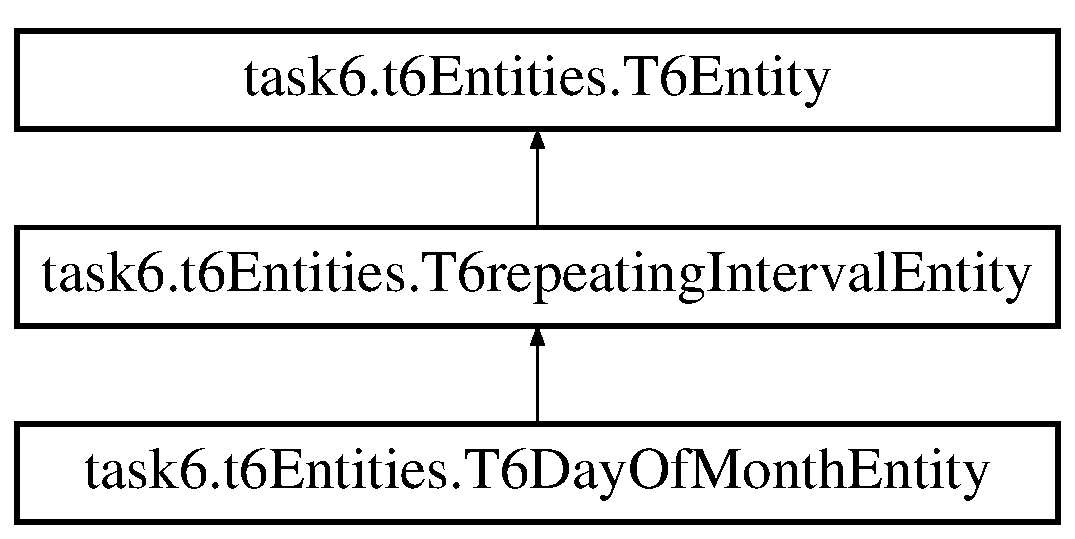
\includegraphics[height=3.000000cm]{classtask6_1_1t6Entities_1_1T6DayOfMonthEntity}
\end{center}
\end{figure}
\subsection*{Public Member Functions}
\begin{DoxyCompactItemize}
\item 
def \hyperlink{classtask6_1_1t6Entities_1_1T6DayOfMonthEntity_a8b5810d8829d1226febe1f06782ff8d9}{\+\_\+\+\_\+init\+\_\+\+\_\+} (self, \hyperlink{classtask6_1_1t6Entities_1_1T6Entity_afeeced8134bb3ebe0cfecc64d0ab46a4}{id}, \hyperlink{classtask6_1_1t6Entities_1_1T6Entity_a52779e9af8864dc98e8b02fc5b9b041a}{start\+\_\+span}, \hyperlink{classtask6_1_1t6Entities_1_1T6Entity_aeb402200b156cd9562c5111dfe777b98}{end\+\_\+span}, \hyperlink{classtask6_1_1t6Entities_1_1T6DayOfMonthEntity_a7b9456d2643595389e1173d6fd711707}{value}, \hyperlink{classtask6_1_1t6Entities_1_1T6DayOfMonthEntity_acdd7f04a1c0cce56487178878ffb5a9f}{sub\+\_\+interval}, \hyperlink{classtask6_1_1t6Entities_1_1T6DayOfMonthEntity_a2eb2f5e038b5a98ce78c3a0dc8f127ac}{number}, \hyperlink{classtask6_1_1t6Entities_1_1T6DayOfMonthEntity_a922d2d4fa863d6c8007a32eace7d97d6}{modifier})
\end{DoxyCompactItemize}
\subsection*{Public Attributes}
\begin{DoxyCompactItemize}
\item 
\hyperlink{classtask6_1_1t6Entities_1_1T6DayOfMonthEntity_a7b9456d2643595389e1173d6fd711707}{value}
\item 
\hyperlink{classtask6_1_1t6Entities_1_1T6DayOfMonthEntity_acdd7f04a1c0cce56487178878ffb5a9f}{sub\+\_\+interval}
\item 
\hyperlink{classtask6_1_1t6Entities_1_1T6DayOfMonthEntity_a2eb2f5e038b5a98ce78c3a0dc8f127ac}{number}
\item 
\hyperlink{classtask6_1_1t6Entities_1_1T6DayOfMonthEntity_a922d2d4fa863d6c8007a32eace7d97d6}{modifier}
\end{DoxyCompactItemize}


\subsection{Detailed Description}


Definition at line 101 of file t6\+Entities.\+py.



\subsection{Constructor \& Destructor Documentation}
\mbox{\Hypertarget{classtask6_1_1t6Entities_1_1T6DayOfMonthEntity_a8b5810d8829d1226febe1f06782ff8d9}\label{classtask6_1_1t6Entities_1_1T6DayOfMonthEntity_a8b5810d8829d1226febe1f06782ff8d9}} 
\index{task6\+::t6\+Entities\+::\+T6\+Day\+Of\+Month\+Entity@{task6\+::t6\+Entities\+::\+T6\+Day\+Of\+Month\+Entity}!\+\_\+\+\_\+init\+\_\+\+\_\+@{\+\_\+\+\_\+init\+\_\+\+\_\+}}
\index{\+\_\+\+\_\+init\+\_\+\+\_\+@{\+\_\+\+\_\+init\+\_\+\+\_\+}!task6\+::t6\+Entities\+::\+T6\+Day\+Of\+Month\+Entity@{task6\+::t6\+Entities\+::\+T6\+Day\+Of\+Month\+Entity}}
\subsubsection{\texorpdfstring{\+\_\+\+\_\+init\+\_\+\+\_\+()}{\_\_init\_\_()}}
{\footnotesize\ttfamily def task6.\+t6\+Entities.\+T6\+Day\+Of\+Month\+Entity.\+\_\+\+\_\+init\+\_\+\+\_\+ (\begin{DoxyParamCaption}\item[{}]{self,  }\item[{}]{id,  }\item[{}]{start\+\_\+span,  }\item[{}]{end\+\_\+span,  }\item[{}]{value,  }\item[{}]{sub\+\_\+interval,  }\item[{}]{number,  }\item[{}]{modifier }\end{DoxyParamCaption})}



Definition at line 102 of file t6\+Entities.\+py.



\subsection{Member Data Documentation}
\mbox{\Hypertarget{classtask6_1_1t6Entities_1_1T6DayOfMonthEntity_a922d2d4fa863d6c8007a32eace7d97d6}\label{classtask6_1_1t6Entities_1_1T6DayOfMonthEntity_a922d2d4fa863d6c8007a32eace7d97d6}} 
\index{task6\+::t6\+Entities\+::\+T6\+Day\+Of\+Month\+Entity@{task6\+::t6\+Entities\+::\+T6\+Day\+Of\+Month\+Entity}!modifier@{modifier}}
\index{modifier@{modifier}!task6\+::t6\+Entities\+::\+T6\+Day\+Of\+Month\+Entity@{task6\+::t6\+Entities\+::\+T6\+Day\+Of\+Month\+Entity}}
\subsubsection{\texorpdfstring{modifier}{modifier}}
{\footnotesize\ttfamily task6.\+t6\+Entities.\+T6\+Day\+Of\+Month\+Entity.\+modifier}



Definition at line 107 of file t6\+Entities.\+py.

\mbox{\Hypertarget{classtask6_1_1t6Entities_1_1T6DayOfMonthEntity_a2eb2f5e038b5a98ce78c3a0dc8f127ac}\label{classtask6_1_1t6Entities_1_1T6DayOfMonthEntity_a2eb2f5e038b5a98ce78c3a0dc8f127ac}} 
\index{task6\+::t6\+Entities\+::\+T6\+Day\+Of\+Month\+Entity@{task6\+::t6\+Entities\+::\+T6\+Day\+Of\+Month\+Entity}!number@{number}}
\index{number@{number}!task6\+::t6\+Entities\+::\+T6\+Day\+Of\+Month\+Entity@{task6\+::t6\+Entities\+::\+T6\+Day\+Of\+Month\+Entity}}
\subsubsection{\texorpdfstring{number}{number}}
{\footnotesize\ttfamily task6.\+t6\+Entities.\+T6\+Day\+Of\+Month\+Entity.\+number}



Definition at line 106 of file t6\+Entities.\+py.

\mbox{\Hypertarget{classtask6_1_1t6Entities_1_1T6DayOfMonthEntity_acdd7f04a1c0cce56487178878ffb5a9f}\label{classtask6_1_1t6Entities_1_1T6DayOfMonthEntity_acdd7f04a1c0cce56487178878ffb5a9f}} 
\index{task6\+::t6\+Entities\+::\+T6\+Day\+Of\+Month\+Entity@{task6\+::t6\+Entities\+::\+T6\+Day\+Of\+Month\+Entity}!sub\+\_\+interval@{sub\+\_\+interval}}
\index{sub\+\_\+interval@{sub\+\_\+interval}!task6\+::t6\+Entities\+::\+T6\+Day\+Of\+Month\+Entity@{task6\+::t6\+Entities\+::\+T6\+Day\+Of\+Month\+Entity}}
\subsubsection{\texorpdfstring{sub\+\_\+interval}{sub\_interval}}
{\footnotesize\ttfamily task6.\+t6\+Entities.\+T6\+Day\+Of\+Month\+Entity.\+sub\+\_\+interval}



Definition at line 105 of file t6\+Entities.\+py.

\mbox{\Hypertarget{classtask6_1_1t6Entities_1_1T6DayOfMonthEntity_a7b9456d2643595389e1173d6fd711707}\label{classtask6_1_1t6Entities_1_1T6DayOfMonthEntity_a7b9456d2643595389e1173d6fd711707}} 
\index{task6\+::t6\+Entities\+::\+T6\+Day\+Of\+Month\+Entity@{task6\+::t6\+Entities\+::\+T6\+Day\+Of\+Month\+Entity}!value@{value}}
\index{value@{value}!task6\+::t6\+Entities\+::\+T6\+Day\+Of\+Month\+Entity@{task6\+::t6\+Entities\+::\+T6\+Day\+Of\+Month\+Entity}}
\subsubsection{\texorpdfstring{value}{value}}
{\footnotesize\ttfamily task6.\+t6\+Entities.\+T6\+Day\+Of\+Month\+Entity.\+value}



Definition at line 104 of file t6\+Entities.\+py.



The documentation for this class was generated from the following file\+:\begin{DoxyCompactItemize}
\item 
task6/\hyperlink{t6Entities_8py}{t6\+Entities.\+py}\end{DoxyCompactItemize}

\hypertarget{classtask6_1_1t6Entities_1_1T6DayOfWeekEntity}{}\section{task6.\+t6\+Entities.\+T6\+Day\+Of\+Week\+Entity Class Reference}
\label{classtask6_1_1t6Entities_1_1T6DayOfWeekEntity}\index{task6.\+t6\+Entities.\+T6\+Day\+Of\+Week\+Entity@{task6.\+t6\+Entities.\+T6\+Day\+Of\+Week\+Entity}}
Inheritance diagram for task6.\+t6\+Entities.\+T6\+Day\+Of\+Week\+Entity\+:\begin{figure}[H]
\begin{center}
\leavevmode
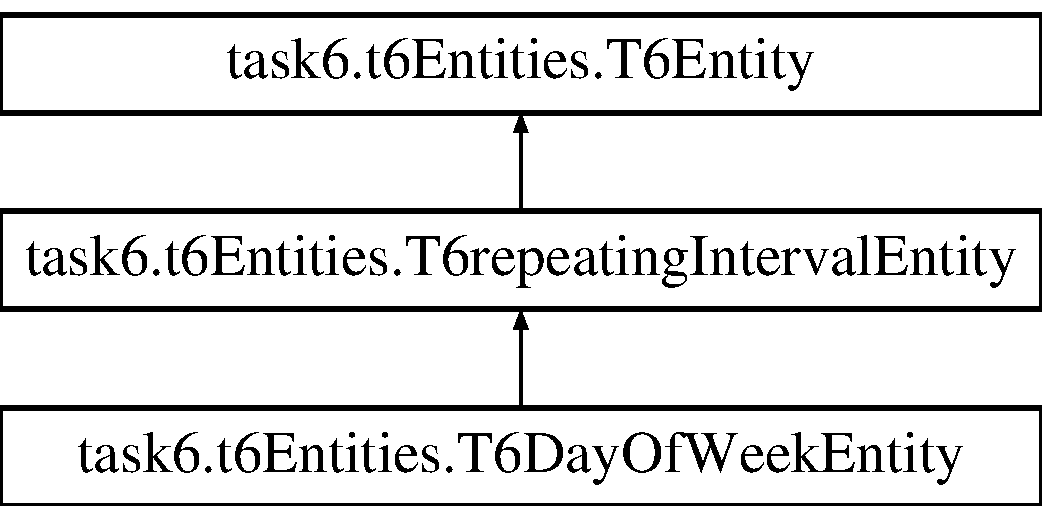
\includegraphics[height=3.000000cm]{classtask6_1_1t6Entities_1_1T6DayOfWeekEntity}
\end{center}
\end{figure}
\subsection*{Public Member Functions}
\begin{DoxyCompactItemize}
\item 
def \hyperlink{classtask6_1_1t6Entities_1_1T6DayOfWeekEntity_a2fc54558a59058cb9da92c440a33f7df}{\+\_\+\+\_\+init\+\_\+\+\_\+} (self, \hyperlink{classtask6_1_1t6Entities_1_1T6Entity_afeeced8134bb3ebe0cfecc64d0ab46a4}{id}, \hyperlink{classtask6_1_1t6Entities_1_1T6Entity_a52779e9af8864dc98e8b02fc5b9b041a}{start\+\_\+span}, \hyperlink{classtask6_1_1t6Entities_1_1T6Entity_aeb402200b156cd9562c5111dfe777b98}{end\+\_\+span}, \hyperlink{classtask6_1_1t6Entities_1_1T6DayOfWeekEntity_a0b096374634bcd3824100aa0b8b03416}{day\+Type}, \hyperlink{classtask6_1_1t6Entities_1_1T6DayOfWeekEntity_a8360936a4d61df06f3e84b74cc96812e}{sub\+\_\+interval}, \hyperlink{classtask6_1_1t6Entities_1_1T6DayOfWeekEntity_a6c4716d536e9be2dba85c5702618b53f}{number}, \hyperlink{classtask6_1_1t6Entities_1_1T6DayOfWeekEntity_a1d18a5075422ee92873d2e995e78a3f7}{modifier})
\end{DoxyCompactItemize}
\subsection*{Public Attributes}
\begin{DoxyCompactItemize}
\item 
\hyperlink{classtask6_1_1t6Entities_1_1T6DayOfWeekEntity_a0b096374634bcd3824100aa0b8b03416}{day\+Type}
\item 
\hyperlink{classtask6_1_1t6Entities_1_1T6DayOfWeekEntity_a8360936a4d61df06f3e84b74cc96812e}{sub\+\_\+interval}
\item 
\hyperlink{classtask6_1_1t6Entities_1_1T6DayOfWeekEntity_a6c4716d536e9be2dba85c5702618b53f}{number}
\item 
\hyperlink{classtask6_1_1t6Entities_1_1T6DayOfWeekEntity_a1d18a5075422ee92873d2e995e78a3f7}{modifier}
\end{DoxyCompactItemize}


\subsection{Detailed Description}


Definition at line 109 of file t6\+Entities.\+py.



\subsection{Constructor \& Destructor Documentation}
\mbox{\Hypertarget{classtask6_1_1t6Entities_1_1T6DayOfWeekEntity_a2fc54558a59058cb9da92c440a33f7df}\label{classtask6_1_1t6Entities_1_1T6DayOfWeekEntity_a2fc54558a59058cb9da92c440a33f7df}} 
\index{task6\+::t6\+Entities\+::\+T6\+Day\+Of\+Week\+Entity@{task6\+::t6\+Entities\+::\+T6\+Day\+Of\+Week\+Entity}!\+\_\+\+\_\+init\+\_\+\+\_\+@{\+\_\+\+\_\+init\+\_\+\+\_\+}}
\index{\+\_\+\+\_\+init\+\_\+\+\_\+@{\+\_\+\+\_\+init\+\_\+\+\_\+}!task6\+::t6\+Entities\+::\+T6\+Day\+Of\+Week\+Entity@{task6\+::t6\+Entities\+::\+T6\+Day\+Of\+Week\+Entity}}
\subsubsection{\texorpdfstring{\+\_\+\+\_\+init\+\_\+\+\_\+()}{\_\_init\_\_()}}
{\footnotesize\ttfamily def task6.\+t6\+Entities.\+T6\+Day\+Of\+Week\+Entity.\+\_\+\+\_\+init\+\_\+\+\_\+ (\begin{DoxyParamCaption}\item[{}]{self,  }\item[{}]{id,  }\item[{}]{start\+\_\+span,  }\item[{}]{end\+\_\+span,  }\item[{}]{day\+Type,  }\item[{}]{sub\+\_\+interval,  }\item[{}]{number,  }\item[{}]{modifier }\end{DoxyParamCaption})}



Definition at line 110 of file t6\+Entities.\+py.



\subsection{Member Data Documentation}
\mbox{\Hypertarget{classtask6_1_1t6Entities_1_1T6DayOfWeekEntity_a0b096374634bcd3824100aa0b8b03416}\label{classtask6_1_1t6Entities_1_1T6DayOfWeekEntity_a0b096374634bcd3824100aa0b8b03416}} 
\index{task6\+::t6\+Entities\+::\+T6\+Day\+Of\+Week\+Entity@{task6\+::t6\+Entities\+::\+T6\+Day\+Of\+Week\+Entity}!day\+Type@{day\+Type}}
\index{day\+Type@{day\+Type}!task6\+::t6\+Entities\+::\+T6\+Day\+Of\+Week\+Entity@{task6\+::t6\+Entities\+::\+T6\+Day\+Of\+Week\+Entity}}
\subsubsection{\texorpdfstring{day\+Type}{dayType}}
{\footnotesize\ttfamily task6.\+t6\+Entities.\+T6\+Day\+Of\+Week\+Entity.\+day\+Type}



Definition at line 112 of file t6\+Entities.\+py.

\mbox{\Hypertarget{classtask6_1_1t6Entities_1_1T6DayOfWeekEntity_a1d18a5075422ee92873d2e995e78a3f7}\label{classtask6_1_1t6Entities_1_1T6DayOfWeekEntity_a1d18a5075422ee92873d2e995e78a3f7}} 
\index{task6\+::t6\+Entities\+::\+T6\+Day\+Of\+Week\+Entity@{task6\+::t6\+Entities\+::\+T6\+Day\+Of\+Week\+Entity}!modifier@{modifier}}
\index{modifier@{modifier}!task6\+::t6\+Entities\+::\+T6\+Day\+Of\+Week\+Entity@{task6\+::t6\+Entities\+::\+T6\+Day\+Of\+Week\+Entity}}
\subsubsection{\texorpdfstring{modifier}{modifier}}
{\footnotesize\ttfamily task6.\+t6\+Entities.\+T6\+Day\+Of\+Week\+Entity.\+modifier}



Definition at line 115 of file t6\+Entities.\+py.

\mbox{\Hypertarget{classtask6_1_1t6Entities_1_1T6DayOfWeekEntity_a6c4716d536e9be2dba85c5702618b53f}\label{classtask6_1_1t6Entities_1_1T6DayOfWeekEntity_a6c4716d536e9be2dba85c5702618b53f}} 
\index{task6\+::t6\+Entities\+::\+T6\+Day\+Of\+Week\+Entity@{task6\+::t6\+Entities\+::\+T6\+Day\+Of\+Week\+Entity}!number@{number}}
\index{number@{number}!task6\+::t6\+Entities\+::\+T6\+Day\+Of\+Week\+Entity@{task6\+::t6\+Entities\+::\+T6\+Day\+Of\+Week\+Entity}}
\subsubsection{\texorpdfstring{number}{number}}
{\footnotesize\ttfamily task6.\+t6\+Entities.\+T6\+Day\+Of\+Week\+Entity.\+number}



Definition at line 114 of file t6\+Entities.\+py.

\mbox{\Hypertarget{classtask6_1_1t6Entities_1_1T6DayOfWeekEntity_a8360936a4d61df06f3e84b74cc96812e}\label{classtask6_1_1t6Entities_1_1T6DayOfWeekEntity_a8360936a4d61df06f3e84b74cc96812e}} 
\index{task6\+::t6\+Entities\+::\+T6\+Day\+Of\+Week\+Entity@{task6\+::t6\+Entities\+::\+T6\+Day\+Of\+Week\+Entity}!sub\+\_\+interval@{sub\+\_\+interval}}
\index{sub\+\_\+interval@{sub\+\_\+interval}!task6\+::t6\+Entities\+::\+T6\+Day\+Of\+Week\+Entity@{task6\+::t6\+Entities\+::\+T6\+Day\+Of\+Week\+Entity}}
\subsubsection{\texorpdfstring{sub\+\_\+interval}{sub\_interval}}
{\footnotesize\ttfamily task6.\+t6\+Entities.\+T6\+Day\+Of\+Week\+Entity.\+sub\+\_\+interval}



Definition at line 113 of file t6\+Entities.\+py.



The documentation for this class was generated from the following file\+:\begin{DoxyCompactItemize}
\item 
task6/\hyperlink{t6Entities_8py}{t6\+Entities.\+py}\end{DoxyCompactItemize}

\hypertarget{classtask6_1_1t6Entities_1_1T6DifferenceOperator}{}\section{task6.\+t6\+Entities.\+T6\+Difference\+Operator Class Reference}
\label{classtask6_1_1t6Entities_1_1T6DifferenceOperator}\index{task6.\+t6\+Entities.\+T6\+Difference\+Operator@{task6.\+t6\+Entities.\+T6\+Difference\+Operator}}
Inheritance diagram for task6.\+t6\+Entities.\+T6\+Difference\+Operator\+:\begin{figure}[H]
\begin{center}
\leavevmode
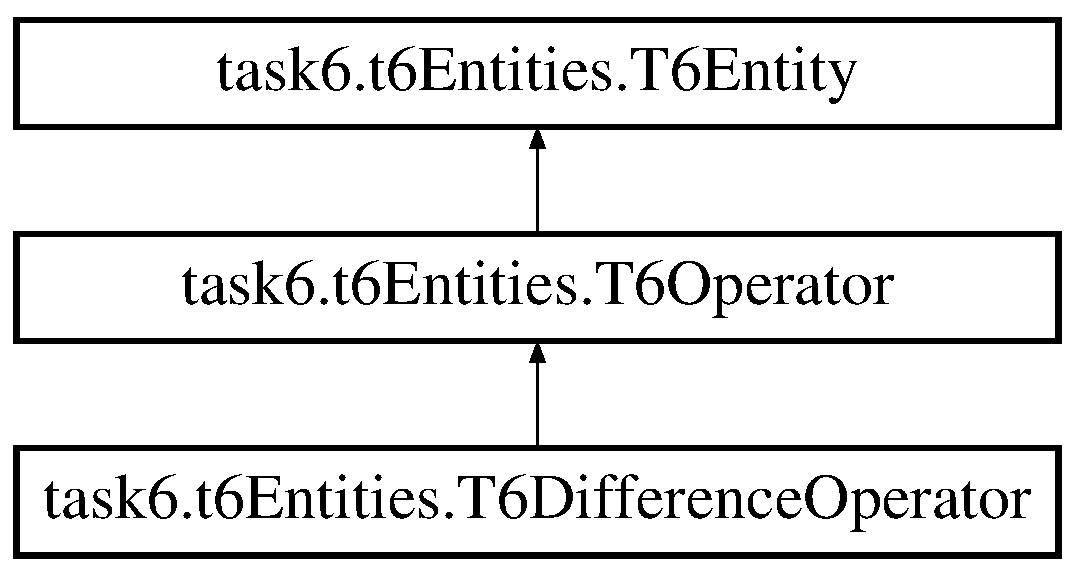
\includegraphics[height=3.000000cm]{classtask6_1_1t6Entities_1_1T6DifferenceOperator}
\end{center}
\end{figure}
\subsection*{Public Member Functions}
\begin{DoxyCompactItemize}
\item 
def \hyperlink{classtask6_1_1t6Entities_1_1T6DifferenceOperator_aabe355d243f7c3cac47bece7cb07f3af}{\+\_\+\+\_\+init\+\_\+\+\_\+} (self, \hyperlink{classtask6_1_1t6Entities_1_1T6Entity_afeeced8134bb3ebe0cfecc64d0ab46a4}{id}, \hyperlink{classtask6_1_1t6Entities_1_1T6Entity_a52779e9af8864dc98e8b02fc5b9b041a}{start\+\_\+span}, \hyperlink{classtask6_1_1t6Entities_1_1T6Entity_aeb402200b156cd9562c5111dfe777b98}{end\+\_\+span})
\end{DoxyCompactItemize}
\subsection*{Additional Inherited Members}


\subsection{Detailed Description}


Definition at line 177 of file t6\+Entities.\+py.



\subsection{Constructor \& Destructor Documentation}
\mbox{\Hypertarget{classtask6_1_1t6Entities_1_1T6DifferenceOperator_aabe355d243f7c3cac47bece7cb07f3af}\label{classtask6_1_1t6Entities_1_1T6DifferenceOperator_aabe355d243f7c3cac47bece7cb07f3af}} 
\index{task6\+::t6\+Entities\+::\+T6\+Difference\+Operator@{task6\+::t6\+Entities\+::\+T6\+Difference\+Operator}!\+\_\+\+\_\+init\+\_\+\+\_\+@{\+\_\+\+\_\+init\+\_\+\+\_\+}}
\index{\+\_\+\+\_\+init\+\_\+\+\_\+@{\+\_\+\+\_\+init\+\_\+\+\_\+}!task6\+::t6\+Entities\+::\+T6\+Difference\+Operator@{task6\+::t6\+Entities\+::\+T6\+Difference\+Operator}}
\subsubsection{\texorpdfstring{\+\_\+\+\_\+init\+\_\+\+\_\+()}{\_\_init\_\_()}}
{\footnotesize\ttfamily def task6.\+t6\+Entities.\+T6\+Difference\+Operator.\+\_\+\+\_\+init\+\_\+\+\_\+ (\begin{DoxyParamCaption}\item[{}]{self,  }\item[{}]{id,  }\item[{}]{start\+\_\+span,  }\item[{}]{end\+\_\+span }\end{DoxyParamCaption})}



Definition at line 178 of file t6\+Entities.\+py.



The documentation for this class was generated from the following file\+:\begin{DoxyCompactItemize}
\item 
task6/\hyperlink{t6Entities_8py}{t6\+Entities.\+py}\end{DoxyCompactItemize}

\hypertarget{classtask6_1_1t6Entities_1_1T6Entity}{}\section{task6.\+t6\+Entities.\+T6\+Entity Class Reference}
\label{classtask6_1_1t6Entities_1_1T6Entity}\index{task6.\+t6\+Entities.\+T6\+Entity@{task6.\+t6\+Entities.\+T6\+Entity}}


Class definitions for all Time\+Norm entities -\/ Intervals, Periods, Repeating-\/\+Intervals, and Operators.  


Inheritance diagram for task6.\+t6\+Entities.\+T6\+Entity\+:\begin{figure}[H]
\begin{center}
\leavevmode
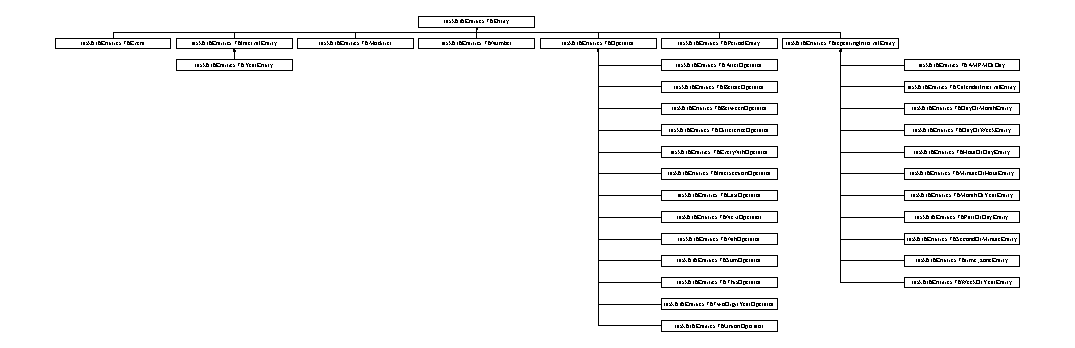
\includegraphics[height=4.233871cm]{classtask6_1_1t6Entities_1_1T6Entity}
\end{center}
\end{figure}
\subsection*{Public Member Functions}
\begin{DoxyCompactItemize}
\item 
def \hyperlink{classtask6_1_1t6Entities_1_1T6Entity_acd7eefda53a955f5a2e2c33331377845}{\+\_\+\+\_\+init\+\_\+\+\_\+} (self, \hyperlink{classtask6_1_1t6Entities_1_1T6Entity_afeeced8134bb3ebe0cfecc64d0ab46a4}{id}, \hyperlink{classtask6_1_1t6Entities_1_1T6Entity_a52779e9af8864dc98e8b02fc5b9b041a}{start\+\_\+span}, \hyperlink{classtask6_1_1t6Entities_1_1T6Entity_aeb402200b156cd9562c5111dfe777b98}{end\+\_\+span}, \hyperlink{classtask6_1_1t6Entities_1_1T6Entity_ae4299399be3ecbd68dbb9ae988bff5a8}{type}, \hyperlink{classtask6_1_1t6Entities_1_1T6Entity_a2e9b6dc858c26a85ad740ad7e1bfda67}{parent\+\_\+type})
\begin{DoxyCompactList}\small\item\em The constructor. \end{DoxyCompactList}\item 
def \hyperlink{classtask6_1_1t6Entities_1_1T6Entity_a4fe9419bea53693abf1b475c88ed5494}{\+\_\+\+\_\+str\+\_\+\+\_\+} (self)
\item 
def \hyperlink{classtask6_1_1t6Entities_1_1T6Entity_aae04121cb00d82840741e39cf0da5706}{set\+\_\+id} (self, \hyperlink{classtask6_1_1t6Entities_1_1T6Entity_afeeced8134bb3ebe0cfecc64d0ab46a4}{id})
\begin{DoxyCompactList}\small\item\em Sets the entity\textquotesingle{}s ID. \end{DoxyCompactList}\item 
def \hyperlink{classtask6_1_1t6Entities_1_1T6Entity_a3b9262436cde3e62dd006ab4986961e1}{get\+\_\+id} (self)
\item 
def \hyperlink{classtask6_1_1t6Entities_1_1T6Entity_a5b8a42787e0d8c65840e69c56eaeeb93}{print\+\_\+string} (self)
\item 
def \hyperlink{classtask6_1_1t6Entities_1_1T6Entity_a3463d49b756cd711c82ce3505521e3ff}{parent\+\_\+type} (self)
\item 
def \hyperlink{classtask6_1_1t6Entities_1_1T6Entity_aadc043ccba4eb2b57cb9ac365dc7dbfe}{print\+\_\+xml} (self)
\begin{DoxyCompactList}\small\item\em Prints the X\+ML representation of the entity. \end{DoxyCompactList}\end{DoxyCompactItemize}
\subsection*{Public Attributes}
\begin{DoxyCompactItemize}
\item 
\hyperlink{classtask6_1_1t6Entities_1_1T6Entity_afeeced8134bb3ebe0cfecc64d0ab46a4}{id}
\item 
\hyperlink{classtask6_1_1t6Entities_1_1T6Entity_a52779e9af8864dc98e8b02fc5b9b041a}{start\+\_\+span}
\item 
\hyperlink{classtask6_1_1t6Entities_1_1T6Entity_aeb402200b156cd9562c5111dfe777b98}{end\+\_\+span}
\item 
\hyperlink{classtask6_1_1t6Entities_1_1T6Entity_ae4299399be3ecbd68dbb9ae988bff5a8}{type}
\item 
\hyperlink{classtask6_1_1t6Entities_1_1T6Entity_a2e9b6dc858c26a85ad740ad7e1bfda67}{parent\+\_\+type}
\end{DoxyCompactItemize}


\subsection{Detailed Description}
Class definitions for all Time\+Norm entities -\/ Intervals, Periods, Repeating-\/\+Intervals, and Operators. 



 Date\+: 9/19/17

Programmer Name\+: Luke Maffey Superclass for all entities

Entities are either an Interval, Period, Repeating-\/\+Interval, or Operator 
\begin{DoxyParams}{Parameters}
{\em id} & Assigned ID number \\
\hline
{\em start\+\_\+span} & The location of the first character \\
\hline
{\em end\+\_\+span} & The location of the last character \\
\hline
{\em type} & The type of the entity \\
\hline
{\em parent\+\_\+type} & The parent type of the entity \\
\hline
\end{DoxyParams}


Definition at line 16 of file t6\+Entities.\+py.



\subsection{Constructor \& Destructor Documentation}
\mbox{\Hypertarget{classtask6_1_1t6Entities_1_1T6Entity_acd7eefda53a955f5a2e2c33331377845}\label{classtask6_1_1t6Entities_1_1T6Entity_acd7eefda53a955f5a2e2c33331377845}} 
\index{task6\+::t6\+Entities\+::\+T6\+Entity@{task6\+::t6\+Entities\+::\+T6\+Entity}!\+\_\+\+\_\+init\+\_\+\+\_\+@{\+\_\+\+\_\+init\+\_\+\+\_\+}}
\index{\+\_\+\+\_\+init\+\_\+\+\_\+@{\+\_\+\+\_\+init\+\_\+\+\_\+}!task6\+::t6\+Entities\+::\+T6\+Entity@{task6\+::t6\+Entities\+::\+T6\+Entity}}
\subsubsection{\texorpdfstring{\+\_\+\+\_\+init\+\_\+\+\_\+()}{\_\_init\_\_()}}
{\footnotesize\ttfamily def task6.\+t6\+Entities.\+T6\+Entity.\+\_\+\+\_\+init\+\_\+\+\_\+ (\begin{DoxyParamCaption}\item[{}]{self,  }\item[{}]{id,  }\item[{}]{start\+\_\+span,  }\item[{}]{end\+\_\+span,  }\item[{}]{type,  }\item[{}]{parent\+\_\+type }\end{DoxyParamCaption})}



The constructor. 



Definition at line 19 of file t6\+Entities.\+py.



\subsection{Member Function Documentation}
\mbox{\Hypertarget{classtask6_1_1t6Entities_1_1T6Entity_a4fe9419bea53693abf1b475c88ed5494}\label{classtask6_1_1t6Entities_1_1T6Entity_a4fe9419bea53693abf1b475c88ed5494}} 
\index{task6\+::t6\+Entities\+::\+T6\+Entity@{task6\+::t6\+Entities\+::\+T6\+Entity}!\+\_\+\+\_\+str\+\_\+\+\_\+@{\+\_\+\+\_\+str\+\_\+\+\_\+}}
\index{\+\_\+\+\_\+str\+\_\+\+\_\+@{\+\_\+\+\_\+str\+\_\+\+\_\+}!task6\+::t6\+Entities\+::\+T6\+Entity@{task6\+::t6\+Entities\+::\+T6\+Entity}}
\subsubsection{\texorpdfstring{\+\_\+\+\_\+str\+\_\+\+\_\+()}{\_\_str\_\_()}}
{\footnotesize\ttfamily def task6.\+t6\+Entities.\+T6\+Entity.\+\_\+\+\_\+str\+\_\+\+\_\+ (\begin{DoxyParamCaption}\item[{}]{self }\end{DoxyParamCaption})}



Definition at line 26 of file t6\+Entities.\+py.

\mbox{\Hypertarget{classtask6_1_1t6Entities_1_1T6Entity_a3b9262436cde3e62dd006ab4986961e1}\label{classtask6_1_1t6Entities_1_1T6Entity_a3b9262436cde3e62dd006ab4986961e1}} 
\index{task6\+::t6\+Entities\+::\+T6\+Entity@{task6\+::t6\+Entities\+::\+T6\+Entity}!get\+\_\+id@{get\+\_\+id}}
\index{get\+\_\+id@{get\+\_\+id}!task6\+::t6\+Entities\+::\+T6\+Entity@{task6\+::t6\+Entities\+::\+T6\+Entity}}
\subsubsection{\texorpdfstring{get\+\_\+id()}{get\_id()}}
{\footnotesize\ttfamily def task6.\+t6\+Entities.\+T6\+Entity.\+get\+\_\+id (\begin{DoxyParamCaption}\item[{}]{self }\end{DoxyParamCaption})}



Definition at line 34 of file t6\+Entities.\+py.

\mbox{\Hypertarget{classtask6_1_1t6Entities_1_1T6Entity_a3463d49b756cd711c82ce3505521e3ff}\label{classtask6_1_1t6Entities_1_1T6Entity_a3463d49b756cd711c82ce3505521e3ff}} 
\index{task6\+::t6\+Entities\+::\+T6\+Entity@{task6\+::t6\+Entities\+::\+T6\+Entity}!parent\+\_\+type@{parent\+\_\+type}}
\index{parent\+\_\+type@{parent\+\_\+type}!task6\+::t6\+Entities\+::\+T6\+Entity@{task6\+::t6\+Entities\+::\+T6\+Entity}}
\subsubsection{\texorpdfstring{parent\+\_\+type()}{parent\_type()}}
{\footnotesize\ttfamily def task6.\+t6\+Entities.\+T6\+Entity.\+parent\+\_\+type (\begin{DoxyParamCaption}\item[{}]{self }\end{DoxyParamCaption})}



Definition at line 40 of file t6\+Entities.\+py.

\mbox{\Hypertarget{classtask6_1_1t6Entities_1_1T6Entity_a5b8a42787e0d8c65840e69c56eaeeb93}\label{classtask6_1_1t6Entities_1_1T6Entity_a5b8a42787e0d8c65840e69c56eaeeb93}} 
\index{task6\+::t6\+Entities\+::\+T6\+Entity@{task6\+::t6\+Entities\+::\+T6\+Entity}!print\+\_\+string@{print\+\_\+string}}
\index{print\+\_\+string@{print\+\_\+string}!task6\+::t6\+Entities\+::\+T6\+Entity@{task6\+::t6\+Entities\+::\+T6\+Entity}}
\subsubsection{\texorpdfstring{print\+\_\+string()}{print\_string()}}
{\footnotesize\ttfamily def task6.\+t6\+Entities.\+T6\+Entity.\+print\+\_\+string (\begin{DoxyParamCaption}\item[{}]{self }\end{DoxyParamCaption})}



Definition at line 37 of file t6\+Entities.\+py.

\mbox{\Hypertarget{classtask6_1_1t6Entities_1_1T6Entity_aadc043ccba4eb2b57cb9ac365dc7dbfe}\label{classtask6_1_1t6Entities_1_1T6Entity_aadc043ccba4eb2b57cb9ac365dc7dbfe}} 
\index{task6\+::t6\+Entities\+::\+T6\+Entity@{task6\+::t6\+Entities\+::\+T6\+Entity}!print\+\_\+xml@{print\+\_\+xml}}
\index{print\+\_\+xml@{print\+\_\+xml}!task6\+::t6\+Entities\+::\+T6\+Entity@{task6\+::t6\+Entities\+::\+T6\+Entity}}
\subsubsection{\texorpdfstring{print\+\_\+xml()}{print\_xml()}}
{\footnotesize\ttfamily def task6.\+t6\+Entities.\+T6\+Entity.\+print\+\_\+xml (\begin{DoxyParamCaption}\item[{}]{self }\end{DoxyParamCaption})}



Prints the X\+ML representation of the entity. 

Subclasses need to close the properties and entities tags 

Definition at line 46 of file t6\+Entities.\+py.

\mbox{\Hypertarget{classtask6_1_1t6Entities_1_1T6Entity_aae04121cb00d82840741e39cf0da5706}\label{classtask6_1_1t6Entities_1_1T6Entity_aae04121cb00d82840741e39cf0da5706}} 
\index{task6\+::t6\+Entities\+::\+T6\+Entity@{task6\+::t6\+Entities\+::\+T6\+Entity}!set\+\_\+id@{set\+\_\+id}}
\index{set\+\_\+id@{set\+\_\+id}!task6\+::t6\+Entities\+::\+T6\+Entity@{task6\+::t6\+Entities\+::\+T6\+Entity}}
\subsubsection{\texorpdfstring{set\+\_\+id()}{set\_id()}}
{\footnotesize\ttfamily def task6.\+t6\+Entities.\+T6\+Entity.\+set\+\_\+id (\begin{DoxyParamCaption}\item[{}]{self,  }\item[{}]{id }\end{DoxyParamCaption})}



Sets the entity\textquotesingle{}s ID. 


\begin{DoxyParams}{Parameters}
{\em id} & The ID to set it to \\
\hline
\end{DoxyParams}


Definition at line 31 of file t6\+Entities.\+py.



\subsection{Member Data Documentation}
\mbox{\Hypertarget{classtask6_1_1t6Entities_1_1T6Entity_aeb402200b156cd9562c5111dfe777b98}\label{classtask6_1_1t6Entities_1_1T6Entity_aeb402200b156cd9562c5111dfe777b98}} 
\index{task6\+::t6\+Entities\+::\+T6\+Entity@{task6\+::t6\+Entities\+::\+T6\+Entity}!end\+\_\+span@{end\+\_\+span}}
\index{end\+\_\+span@{end\+\_\+span}!task6\+::t6\+Entities\+::\+T6\+Entity@{task6\+::t6\+Entities\+::\+T6\+Entity}}
\subsubsection{\texorpdfstring{end\+\_\+span}{end\_span}}
{\footnotesize\ttfamily task6.\+t6\+Entities.\+T6\+Entity.\+end\+\_\+span}



Definition at line 22 of file t6\+Entities.\+py.

\mbox{\Hypertarget{classtask6_1_1t6Entities_1_1T6Entity_afeeced8134bb3ebe0cfecc64d0ab46a4}\label{classtask6_1_1t6Entities_1_1T6Entity_afeeced8134bb3ebe0cfecc64d0ab46a4}} 
\index{task6\+::t6\+Entities\+::\+T6\+Entity@{task6\+::t6\+Entities\+::\+T6\+Entity}!id@{id}}
\index{id@{id}!task6\+::t6\+Entities\+::\+T6\+Entity@{task6\+::t6\+Entities\+::\+T6\+Entity}}
\subsubsection{\texorpdfstring{id}{id}}
{\footnotesize\ttfamily task6.\+t6\+Entities.\+T6\+Entity.\+id}



Definition at line 20 of file t6\+Entities.\+py.

\mbox{\Hypertarget{classtask6_1_1t6Entities_1_1T6Entity_a2e9b6dc858c26a85ad740ad7e1bfda67}\label{classtask6_1_1t6Entities_1_1T6Entity_a2e9b6dc858c26a85ad740ad7e1bfda67}} 
\index{task6\+::t6\+Entities\+::\+T6\+Entity@{task6\+::t6\+Entities\+::\+T6\+Entity}!parent\+\_\+type@{parent\+\_\+type}}
\index{parent\+\_\+type@{parent\+\_\+type}!task6\+::t6\+Entities\+::\+T6\+Entity@{task6\+::t6\+Entities\+::\+T6\+Entity}}
\subsubsection{\texorpdfstring{parent\+\_\+type}{parent\_type}}
{\footnotesize\ttfamily task6.\+t6\+Entities.\+T6\+Entity.\+parent\+\_\+type}



Definition at line 24 of file t6\+Entities.\+py.

\mbox{\Hypertarget{classtask6_1_1t6Entities_1_1T6Entity_a52779e9af8864dc98e8b02fc5b9b041a}\label{classtask6_1_1t6Entities_1_1T6Entity_a52779e9af8864dc98e8b02fc5b9b041a}} 
\index{task6\+::t6\+Entities\+::\+T6\+Entity@{task6\+::t6\+Entities\+::\+T6\+Entity}!start\+\_\+span@{start\+\_\+span}}
\index{start\+\_\+span@{start\+\_\+span}!task6\+::t6\+Entities\+::\+T6\+Entity@{task6\+::t6\+Entities\+::\+T6\+Entity}}
\subsubsection{\texorpdfstring{start\+\_\+span}{start\_span}}
{\footnotesize\ttfamily task6.\+t6\+Entities.\+T6\+Entity.\+start\+\_\+span}



Definition at line 21 of file t6\+Entities.\+py.

\mbox{\Hypertarget{classtask6_1_1t6Entities_1_1T6Entity_ae4299399be3ecbd68dbb9ae988bff5a8}\label{classtask6_1_1t6Entities_1_1T6Entity_ae4299399be3ecbd68dbb9ae988bff5a8}} 
\index{task6\+::t6\+Entities\+::\+T6\+Entity@{task6\+::t6\+Entities\+::\+T6\+Entity}!type@{type}}
\index{type@{type}!task6\+::t6\+Entities\+::\+T6\+Entity@{task6\+::t6\+Entities\+::\+T6\+Entity}}
\subsubsection{\texorpdfstring{type}{type}}
{\footnotesize\ttfamily task6.\+t6\+Entities.\+T6\+Entity.\+type}



Definition at line 23 of file t6\+Entities.\+py.



The documentation for this class was generated from the following file\+:\begin{DoxyCompactItemize}
\item 
task6/\hyperlink{t6Entities_8py}{t6\+Entities.\+py}\end{DoxyCompactItemize}

\hypertarget{classtask6_1_1t6Entities_1_1T6Event}{}\section{task6.\+t6\+Entities.\+T6\+Event Class Reference}
\label{classtask6_1_1t6Entities_1_1T6Event}\index{task6.\+t6\+Entities.\+T6\+Event@{task6.\+t6\+Entities.\+T6\+Event}}
Inheritance diagram for task6.\+t6\+Entities.\+T6\+Event\+:\begin{figure}[H]
\begin{center}
\leavevmode
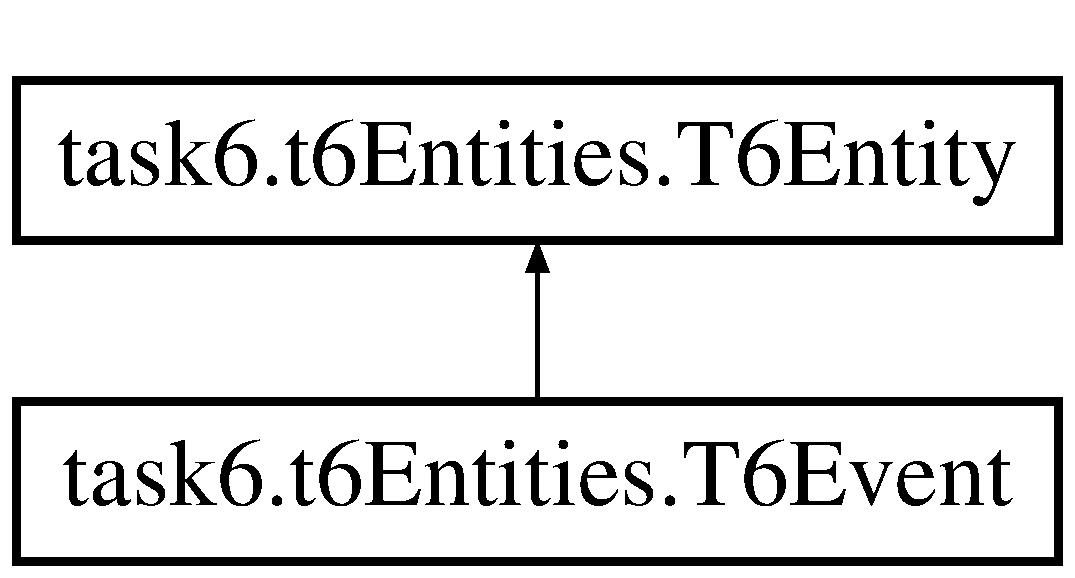
\includegraphics[height=2.000000cm]{classtask6_1_1t6Entities_1_1T6Event}
\end{center}
\end{figure}
\subsection*{Public Member Functions}
\begin{DoxyCompactItemize}
\item 
def \hyperlink{classtask6_1_1t6Entities_1_1T6Event_a00594e097d608a203004934593b9faa9}{\+\_\+\+\_\+init\+\_\+\+\_\+} (self, \hyperlink{classtask6_1_1t6Entities_1_1T6Entity_afeeced8134bb3ebe0cfecc64d0ab46a4}{id}, \hyperlink{classtask6_1_1t6Entities_1_1T6Entity_a52779e9af8864dc98e8b02fc5b9b041a}{start\+\_\+span}, \hyperlink{classtask6_1_1t6Entities_1_1T6Entity_aeb402200b156cd9562c5111dfe777b98}{end\+\_\+span})
\end{DoxyCompactItemize}
\subsection*{Additional Inherited Members}


\subsection{Detailed Description}


Definition at line 277 of file t6\+Entities.\+py.



\subsection{Constructor \& Destructor Documentation}
\mbox{\Hypertarget{classtask6_1_1t6Entities_1_1T6Event_a00594e097d608a203004934593b9faa9}\label{classtask6_1_1t6Entities_1_1T6Event_a00594e097d608a203004934593b9faa9}} 
\index{task6\+::t6\+Entities\+::\+T6\+Event@{task6\+::t6\+Entities\+::\+T6\+Event}!\+\_\+\+\_\+init\+\_\+\+\_\+@{\+\_\+\+\_\+init\+\_\+\+\_\+}}
\index{\+\_\+\+\_\+init\+\_\+\+\_\+@{\+\_\+\+\_\+init\+\_\+\+\_\+}!task6\+::t6\+Entities\+::\+T6\+Event@{task6\+::t6\+Entities\+::\+T6\+Event}}
\subsubsection{\texorpdfstring{\+\_\+\+\_\+init\+\_\+\+\_\+()}{\_\_init\_\_()}}
{\footnotesize\ttfamily def task6.\+t6\+Entities.\+T6\+Event.\+\_\+\+\_\+init\+\_\+\+\_\+ (\begin{DoxyParamCaption}\item[{}]{self,  }\item[{}]{id,  }\item[{}]{start\+\_\+span,  }\item[{}]{end\+\_\+span }\end{DoxyParamCaption})}



Definition at line 278 of file t6\+Entities.\+py.



The documentation for this class was generated from the following file\+:\begin{DoxyCompactItemize}
\item 
task6/\hyperlink{t6Entities_8py}{t6\+Entities.\+py}\end{DoxyCompactItemize}

\hypertarget{classtask6_1_1t6Entities_1_1T6EveryNthOperator}{}\section{task6.\+t6\+Entities.\+T6\+Every\+Nth\+Operator Class Reference}
\label{classtask6_1_1t6Entities_1_1T6EveryNthOperator}\index{task6.\+t6\+Entities.\+T6\+Every\+Nth\+Operator@{task6.\+t6\+Entities.\+T6\+Every\+Nth\+Operator}}
Inheritance diagram for task6.\+t6\+Entities.\+T6\+Every\+Nth\+Operator\+:\begin{figure}[H]
\begin{center}
\leavevmode
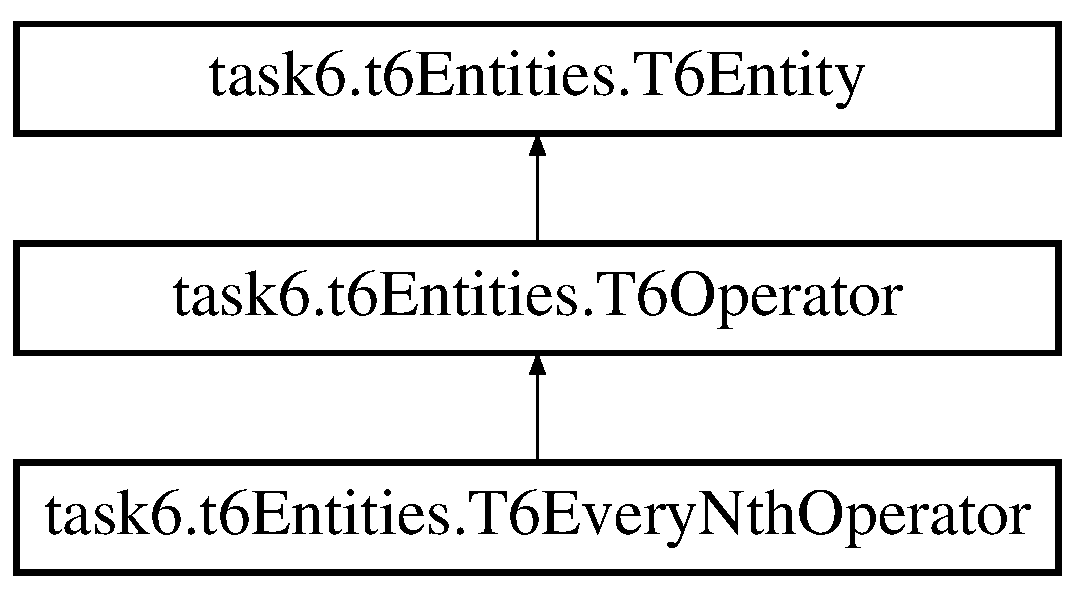
\includegraphics[height=3.000000cm]{classtask6_1_1t6Entities_1_1T6EveryNthOperator}
\end{center}
\end{figure}
\subsection*{Public Member Functions}
\begin{DoxyCompactItemize}
\item 
def \hyperlink{classtask6_1_1t6Entities_1_1T6EveryNthOperator_a0a776eb2a3e12e280405a629eb0fc2e4}{\+\_\+\+\_\+init\+\_\+\+\_\+} (self, \hyperlink{classtask6_1_1t6Entities_1_1T6Entity_afeeced8134bb3ebe0cfecc64d0ab46a4}{id}, \hyperlink{classtask6_1_1t6Entities_1_1T6Entity_a52779e9af8864dc98e8b02fc5b9b041a}{start\+\_\+span}, \hyperlink{classtask6_1_1t6Entities_1_1T6Entity_aeb402200b156cd9562c5111dfe777b98}{end\+\_\+span})
\end{DoxyCompactItemize}
\subsection*{Additional Inherited Members}


\subsection{Detailed Description}


Definition at line 194 of file t6\+Entities.\+py.



\subsection{Constructor \& Destructor Documentation}
\mbox{\Hypertarget{classtask6_1_1t6Entities_1_1T6EveryNthOperator_a0a776eb2a3e12e280405a629eb0fc2e4}\label{classtask6_1_1t6Entities_1_1T6EveryNthOperator_a0a776eb2a3e12e280405a629eb0fc2e4}} 
\index{task6\+::t6\+Entities\+::\+T6\+Every\+Nth\+Operator@{task6\+::t6\+Entities\+::\+T6\+Every\+Nth\+Operator}!\+\_\+\+\_\+init\+\_\+\+\_\+@{\+\_\+\+\_\+init\+\_\+\+\_\+}}
\index{\+\_\+\+\_\+init\+\_\+\+\_\+@{\+\_\+\+\_\+init\+\_\+\+\_\+}!task6\+::t6\+Entities\+::\+T6\+Every\+Nth\+Operator@{task6\+::t6\+Entities\+::\+T6\+Every\+Nth\+Operator}}
\subsubsection{\texorpdfstring{\+\_\+\+\_\+init\+\_\+\+\_\+()}{\_\_init\_\_()}}
{\footnotesize\ttfamily def task6.\+t6\+Entities.\+T6\+Every\+Nth\+Operator.\+\_\+\+\_\+init\+\_\+\+\_\+ (\begin{DoxyParamCaption}\item[{}]{self,  }\item[{}]{id,  }\item[{}]{start\+\_\+span,  }\item[{}]{end\+\_\+span }\end{DoxyParamCaption})}



Definition at line 195 of file t6\+Entities.\+py.



The documentation for this class was generated from the following file\+:\begin{DoxyCompactItemize}
\item 
task6/\hyperlink{t6Entities_8py}{t6\+Entities.\+py}\end{DoxyCompactItemize}

\hypertarget{classtask6_1_1t6Entities_1_1T6HourOfDayEntity}{}\section{task6.\+t6\+Entities.\+T6\+Hour\+Of\+Day\+Entity Class Reference}
\label{classtask6_1_1t6Entities_1_1T6HourOfDayEntity}\index{task6.\+t6\+Entities.\+T6\+Hour\+Of\+Day\+Entity@{task6.\+t6\+Entities.\+T6\+Hour\+Of\+Day\+Entity}}
Inheritance diagram for task6.\+t6\+Entities.\+T6\+Hour\+Of\+Day\+Entity\+:\begin{figure}[H]
\begin{center}
\leavevmode
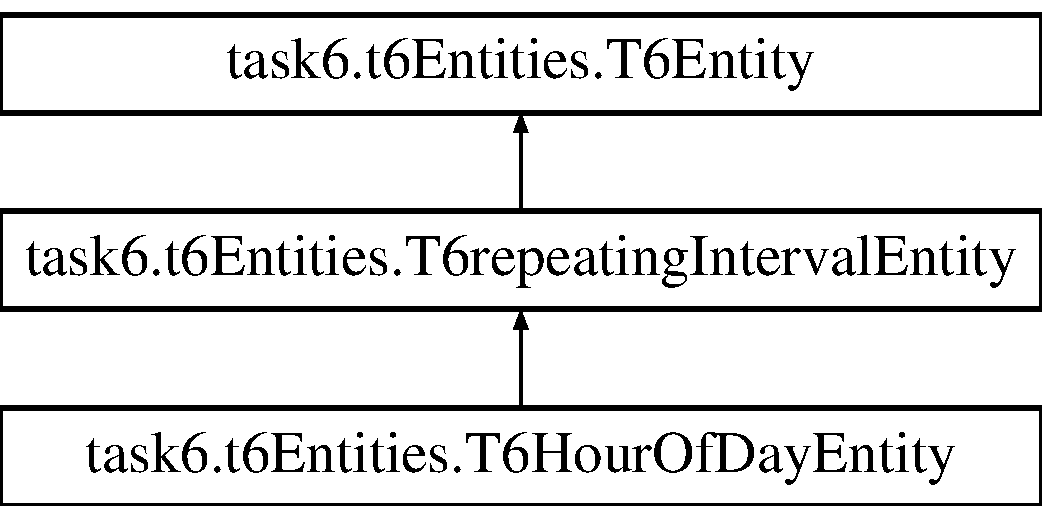
\includegraphics[height=3.000000cm]{classtask6_1_1t6Entities_1_1T6HourOfDayEntity}
\end{center}
\end{figure}
\subsection*{Public Member Functions}
\begin{DoxyCompactItemize}
\item 
def \hyperlink{classtask6_1_1t6Entities_1_1T6HourOfDayEntity_a0a375307b245c7408ae1bbaec1585dc1}{\+\_\+\+\_\+init\+\_\+\+\_\+} (self, \hyperlink{classtask6_1_1t6Entities_1_1T6Entity_afeeced8134bb3ebe0cfecc64d0ab46a4}{id}, \hyperlink{classtask6_1_1t6Entities_1_1T6Entity_a52779e9af8864dc98e8b02fc5b9b041a}{start\+\_\+span}, \hyperlink{classtask6_1_1t6Entities_1_1T6Entity_aeb402200b156cd9562c5111dfe777b98}{end\+\_\+span}, \hyperlink{classtask6_1_1t6Entities_1_1T6HourOfDayEntity_aca30067d70324692cc16ad71cc422dec}{value}, \hyperlink{classtask6_1_1t6Entities_1_1T6HourOfDayEntity_a79df4da1e3285cf9c75ca102c631bd71}{ampm}, \hyperlink{classtask6_1_1t6Entities_1_1T6HourOfDayEntity_ac288e691b6a5181108729f0f1d8c0e84}{time\+\_\+zone}, \hyperlink{classtask6_1_1t6Entities_1_1T6HourOfDayEntity_afe660c17ee2ca754246bf4b931361e4b}{sub\+\_\+interval}, \hyperlink{classtask6_1_1t6Entities_1_1T6HourOfDayEntity_a9f57727fe8828f891028e9e0f856236d}{number}, \hyperlink{classtask6_1_1t6Entities_1_1T6HourOfDayEntity_ab670222d263a06375a37059e8bb8026d}{modifier})
\end{DoxyCompactItemize}
\subsection*{Public Attributes}
\begin{DoxyCompactItemize}
\item 
\hyperlink{classtask6_1_1t6Entities_1_1T6HourOfDayEntity_aca30067d70324692cc16ad71cc422dec}{value}
\item 
\hyperlink{classtask6_1_1t6Entities_1_1T6HourOfDayEntity_a79df4da1e3285cf9c75ca102c631bd71}{ampm}
\item 
\hyperlink{classtask6_1_1t6Entities_1_1T6HourOfDayEntity_ac288e691b6a5181108729f0f1d8c0e84}{time\+\_\+zone}
\item 
\hyperlink{classtask6_1_1t6Entities_1_1T6HourOfDayEntity_afe660c17ee2ca754246bf4b931361e4b}{sub\+\_\+interval}
\item 
\hyperlink{classtask6_1_1t6Entities_1_1T6HourOfDayEntity_a9f57727fe8828f891028e9e0f856236d}{number}
\item 
\hyperlink{classtask6_1_1t6Entities_1_1T6HourOfDayEntity_ab670222d263a06375a37059e8bb8026d}{modifier}
\end{DoxyCompactItemize}


\subsection{Detailed Description}


Definition at line 117 of file t6\+Entities.\+py.



\subsection{Constructor \& Destructor Documentation}
\mbox{\Hypertarget{classtask6_1_1t6Entities_1_1T6HourOfDayEntity_a0a375307b245c7408ae1bbaec1585dc1}\label{classtask6_1_1t6Entities_1_1T6HourOfDayEntity_a0a375307b245c7408ae1bbaec1585dc1}} 
\index{task6\+::t6\+Entities\+::\+T6\+Hour\+Of\+Day\+Entity@{task6\+::t6\+Entities\+::\+T6\+Hour\+Of\+Day\+Entity}!\+\_\+\+\_\+init\+\_\+\+\_\+@{\+\_\+\+\_\+init\+\_\+\+\_\+}}
\index{\+\_\+\+\_\+init\+\_\+\+\_\+@{\+\_\+\+\_\+init\+\_\+\+\_\+}!task6\+::t6\+Entities\+::\+T6\+Hour\+Of\+Day\+Entity@{task6\+::t6\+Entities\+::\+T6\+Hour\+Of\+Day\+Entity}}
\subsubsection{\texorpdfstring{\+\_\+\+\_\+init\+\_\+\+\_\+()}{\_\_init\_\_()}}
{\footnotesize\ttfamily def task6.\+t6\+Entities.\+T6\+Hour\+Of\+Day\+Entity.\+\_\+\+\_\+init\+\_\+\+\_\+ (\begin{DoxyParamCaption}\item[{}]{self,  }\item[{}]{id,  }\item[{}]{start\+\_\+span,  }\item[{}]{end\+\_\+span,  }\item[{}]{value,  }\item[{}]{ampm,  }\item[{}]{time\+\_\+zone,  }\item[{}]{sub\+\_\+interval,  }\item[{}]{number,  }\item[{}]{modifier }\end{DoxyParamCaption})}



Definition at line 118 of file t6\+Entities.\+py.



\subsection{Member Data Documentation}
\mbox{\Hypertarget{classtask6_1_1t6Entities_1_1T6HourOfDayEntity_a79df4da1e3285cf9c75ca102c631bd71}\label{classtask6_1_1t6Entities_1_1T6HourOfDayEntity_a79df4da1e3285cf9c75ca102c631bd71}} 
\index{task6\+::t6\+Entities\+::\+T6\+Hour\+Of\+Day\+Entity@{task6\+::t6\+Entities\+::\+T6\+Hour\+Of\+Day\+Entity}!ampm@{ampm}}
\index{ampm@{ampm}!task6\+::t6\+Entities\+::\+T6\+Hour\+Of\+Day\+Entity@{task6\+::t6\+Entities\+::\+T6\+Hour\+Of\+Day\+Entity}}
\subsubsection{\texorpdfstring{ampm}{ampm}}
{\footnotesize\ttfamily task6.\+t6\+Entities.\+T6\+Hour\+Of\+Day\+Entity.\+ampm}



Definition at line 121 of file t6\+Entities.\+py.

\mbox{\Hypertarget{classtask6_1_1t6Entities_1_1T6HourOfDayEntity_ab670222d263a06375a37059e8bb8026d}\label{classtask6_1_1t6Entities_1_1T6HourOfDayEntity_ab670222d263a06375a37059e8bb8026d}} 
\index{task6\+::t6\+Entities\+::\+T6\+Hour\+Of\+Day\+Entity@{task6\+::t6\+Entities\+::\+T6\+Hour\+Of\+Day\+Entity}!modifier@{modifier}}
\index{modifier@{modifier}!task6\+::t6\+Entities\+::\+T6\+Hour\+Of\+Day\+Entity@{task6\+::t6\+Entities\+::\+T6\+Hour\+Of\+Day\+Entity}}
\subsubsection{\texorpdfstring{modifier}{modifier}}
{\footnotesize\ttfamily task6.\+t6\+Entities.\+T6\+Hour\+Of\+Day\+Entity.\+modifier}



Definition at line 125 of file t6\+Entities.\+py.

\mbox{\Hypertarget{classtask6_1_1t6Entities_1_1T6HourOfDayEntity_a9f57727fe8828f891028e9e0f856236d}\label{classtask6_1_1t6Entities_1_1T6HourOfDayEntity_a9f57727fe8828f891028e9e0f856236d}} 
\index{task6\+::t6\+Entities\+::\+T6\+Hour\+Of\+Day\+Entity@{task6\+::t6\+Entities\+::\+T6\+Hour\+Of\+Day\+Entity}!number@{number}}
\index{number@{number}!task6\+::t6\+Entities\+::\+T6\+Hour\+Of\+Day\+Entity@{task6\+::t6\+Entities\+::\+T6\+Hour\+Of\+Day\+Entity}}
\subsubsection{\texorpdfstring{number}{number}}
{\footnotesize\ttfamily task6.\+t6\+Entities.\+T6\+Hour\+Of\+Day\+Entity.\+number}



Definition at line 124 of file t6\+Entities.\+py.

\mbox{\Hypertarget{classtask6_1_1t6Entities_1_1T6HourOfDayEntity_afe660c17ee2ca754246bf4b931361e4b}\label{classtask6_1_1t6Entities_1_1T6HourOfDayEntity_afe660c17ee2ca754246bf4b931361e4b}} 
\index{task6\+::t6\+Entities\+::\+T6\+Hour\+Of\+Day\+Entity@{task6\+::t6\+Entities\+::\+T6\+Hour\+Of\+Day\+Entity}!sub\+\_\+interval@{sub\+\_\+interval}}
\index{sub\+\_\+interval@{sub\+\_\+interval}!task6\+::t6\+Entities\+::\+T6\+Hour\+Of\+Day\+Entity@{task6\+::t6\+Entities\+::\+T6\+Hour\+Of\+Day\+Entity}}
\subsubsection{\texorpdfstring{sub\+\_\+interval}{sub\_interval}}
{\footnotesize\ttfamily task6.\+t6\+Entities.\+T6\+Hour\+Of\+Day\+Entity.\+sub\+\_\+interval}



Definition at line 123 of file t6\+Entities.\+py.

\mbox{\Hypertarget{classtask6_1_1t6Entities_1_1T6HourOfDayEntity_ac288e691b6a5181108729f0f1d8c0e84}\label{classtask6_1_1t6Entities_1_1T6HourOfDayEntity_ac288e691b6a5181108729f0f1d8c0e84}} 
\index{task6\+::t6\+Entities\+::\+T6\+Hour\+Of\+Day\+Entity@{task6\+::t6\+Entities\+::\+T6\+Hour\+Of\+Day\+Entity}!time\+\_\+zone@{time\+\_\+zone}}
\index{time\+\_\+zone@{time\+\_\+zone}!task6\+::t6\+Entities\+::\+T6\+Hour\+Of\+Day\+Entity@{task6\+::t6\+Entities\+::\+T6\+Hour\+Of\+Day\+Entity}}
\subsubsection{\texorpdfstring{time\+\_\+zone}{time\_zone}}
{\footnotesize\ttfamily task6.\+t6\+Entities.\+T6\+Hour\+Of\+Day\+Entity.\+time\+\_\+zone}



Definition at line 122 of file t6\+Entities.\+py.

\mbox{\Hypertarget{classtask6_1_1t6Entities_1_1T6HourOfDayEntity_aca30067d70324692cc16ad71cc422dec}\label{classtask6_1_1t6Entities_1_1T6HourOfDayEntity_aca30067d70324692cc16ad71cc422dec}} 
\index{task6\+::t6\+Entities\+::\+T6\+Hour\+Of\+Day\+Entity@{task6\+::t6\+Entities\+::\+T6\+Hour\+Of\+Day\+Entity}!value@{value}}
\index{value@{value}!task6\+::t6\+Entities\+::\+T6\+Hour\+Of\+Day\+Entity@{task6\+::t6\+Entities\+::\+T6\+Hour\+Of\+Day\+Entity}}
\subsubsection{\texorpdfstring{value}{value}}
{\footnotesize\ttfamily task6.\+t6\+Entities.\+T6\+Hour\+Of\+Day\+Entity.\+value}



Definition at line 120 of file t6\+Entities.\+py.



The documentation for this class was generated from the following file\+:\begin{DoxyCompactItemize}
\item 
task6/\hyperlink{t6Entities_8py}{t6\+Entities.\+py}\end{DoxyCompactItemize}

\hypertarget{classtask6_1_1t6Entities_1_1T6IntersectionOperator}{}\section{task6.\+t6\+Entities.\+T6\+Intersection\+Operator Class Reference}
\label{classtask6_1_1t6Entities_1_1T6IntersectionOperator}\index{task6.\+t6\+Entities.\+T6\+Intersection\+Operator@{task6.\+t6\+Entities.\+T6\+Intersection\+Operator}}
Inheritance diagram for task6.\+t6\+Entities.\+T6\+Intersection\+Operator\+:\begin{figure}[H]
\begin{center}
\leavevmode
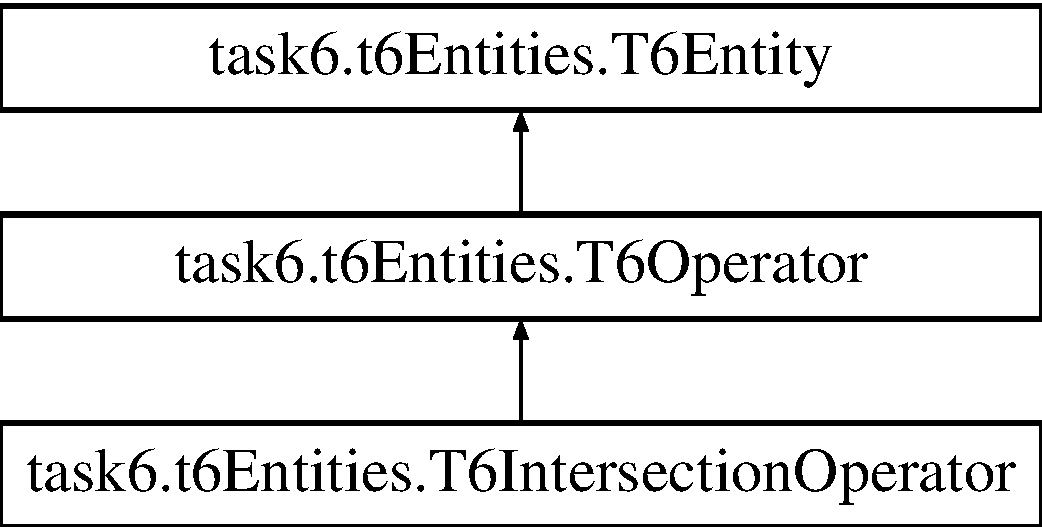
\includegraphics[height=3.000000cm]{classtask6_1_1t6Entities_1_1T6IntersectionOperator}
\end{center}
\end{figure}
\subsection*{Public Member Functions}
\begin{DoxyCompactItemize}
\item 
def \hyperlink{classtask6_1_1t6Entities_1_1T6IntersectionOperator_a09d2c525342b096bbbff094dfb3ba3ac}{\+\_\+\+\_\+init\+\_\+\+\_\+} (self, \hyperlink{classtask6_1_1t6Entities_1_1T6Entity_afeeced8134bb3ebe0cfecc64d0ab46a4}{id}, \hyperlink{classtask6_1_1t6Entities_1_1T6Entity_a52779e9af8864dc98e8b02fc5b9b041a}{start\+\_\+span}, \hyperlink{classtask6_1_1t6Entities_1_1T6Entity_aeb402200b156cd9562c5111dfe777b98}{end\+\_\+span}, \hyperlink{classtask6_1_1t6Entities_1_1T6IntersectionOperator_ad0babf5eab389a9e9d48109f2db05dc2}{intervals}, \hyperlink{classtask6_1_1t6Entities_1_1T6IntersectionOperator_ad8792e2967320f1650f5f51ea1d416f3}{repeating\+\_\+intervals})
\end{DoxyCompactItemize}
\subsection*{Public Attributes}
\begin{DoxyCompactItemize}
\item 
\hyperlink{classtask6_1_1t6Entities_1_1T6IntersectionOperator_ad0babf5eab389a9e9d48109f2db05dc2}{intervals}
\item 
\hyperlink{classtask6_1_1t6Entities_1_1T6IntersectionOperator_ad8792e2967320f1650f5f51ea1d416f3}{repeating\+\_\+intervals}
\end{DoxyCompactItemize}


\subsection{Detailed Description}


Definition at line 187 of file t6\+Entities.\+py.



\subsection{Constructor \& Destructor Documentation}
\mbox{\Hypertarget{classtask6_1_1t6Entities_1_1T6IntersectionOperator_a09d2c525342b096bbbff094dfb3ba3ac}\label{classtask6_1_1t6Entities_1_1T6IntersectionOperator_a09d2c525342b096bbbff094dfb3ba3ac}} 
\index{task6\+::t6\+Entities\+::\+T6\+Intersection\+Operator@{task6\+::t6\+Entities\+::\+T6\+Intersection\+Operator}!\+\_\+\+\_\+init\+\_\+\+\_\+@{\+\_\+\+\_\+init\+\_\+\+\_\+}}
\index{\+\_\+\+\_\+init\+\_\+\+\_\+@{\+\_\+\+\_\+init\+\_\+\+\_\+}!task6\+::t6\+Entities\+::\+T6\+Intersection\+Operator@{task6\+::t6\+Entities\+::\+T6\+Intersection\+Operator}}
\subsubsection{\texorpdfstring{\+\_\+\+\_\+init\+\_\+\+\_\+()}{\_\_init\_\_()}}
{\footnotesize\ttfamily def task6.\+t6\+Entities.\+T6\+Intersection\+Operator.\+\_\+\+\_\+init\+\_\+\+\_\+ (\begin{DoxyParamCaption}\item[{}]{self,  }\item[{}]{id,  }\item[{}]{start\+\_\+span,  }\item[{}]{end\+\_\+span,  }\item[{}]{intervals,  }\item[{}]{repeating\+\_\+intervals }\end{DoxyParamCaption})}



Definition at line 188 of file t6\+Entities.\+py.



\subsection{Member Data Documentation}
\mbox{\Hypertarget{classtask6_1_1t6Entities_1_1T6IntersectionOperator_ad0babf5eab389a9e9d48109f2db05dc2}\label{classtask6_1_1t6Entities_1_1T6IntersectionOperator_ad0babf5eab389a9e9d48109f2db05dc2}} 
\index{task6\+::t6\+Entities\+::\+T6\+Intersection\+Operator@{task6\+::t6\+Entities\+::\+T6\+Intersection\+Operator}!intervals@{intervals}}
\index{intervals@{intervals}!task6\+::t6\+Entities\+::\+T6\+Intersection\+Operator@{task6\+::t6\+Entities\+::\+T6\+Intersection\+Operator}}
\subsubsection{\texorpdfstring{intervals}{intervals}}
{\footnotesize\ttfamily task6.\+t6\+Entities.\+T6\+Intersection\+Operator.\+intervals}



Definition at line 190 of file t6\+Entities.\+py.

\mbox{\Hypertarget{classtask6_1_1t6Entities_1_1T6IntersectionOperator_ad8792e2967320f1650f5f51ea1d416f3}\label{classtask6_1_1t6Entities_1_1T6IntersectionOperator_ad8792e2967320f1650f5f51ea1d416f3}} 
\index{task6\+::t6\+Entities\+::\+T6\+Intersection\+Operator@{task6\+::t6\+Entities\+::\+T6\+Intersection\+Operator}!repeating\+\_\+intervals@{repeating\+\_\+intervals}}
\index{repeating\+\_\+intervals@{repeating\+\_\+intervals}!task6\+::t6\+Entities\+::\+T6\+Intersection\+Operator@{task6\+::t6\+Entities\+::\+T6\+Intersection\+Operator}}
\subsubsection{\texorpdfstring{repeating\+\_\+intervals}{repeating\_intervals}}
{\footnotesize\ttfamily task6.\+t6\+Entities.\+T6\+Intersection\+Operator.\+repeating\+\_\+intervals}



Definition at line 191 of file t6\+Entities.\+py.



The documentation for this class was generated from the following file\+:\begin{DoxyCompactItemize}
\item 
task6/\hyperlink{t6Entities_8py}{t6\+Entities.\+py}\end{DoxyCompactItemize}

\hypertarget{classtask6_1_1t6Entities_1_1T6IntervalEntity}{}\section{task6.\+t6\+Entities.\+T6\+Interval\+Entity Class Reference}
\label{classtask6_1_1t6Entities_1_1T6IntervalEntity}\index{task6.\+t6\+Entities.\+T6\+Interval\+Entity@{task6.\+t6\+Entities.\+T6\+Interval\+Entity}}


An interval, just super classes for year interval for consistency.  


Inheritance diagram for task6.\+t6\+Entities.\+T6\+Interval\+Entity\+:\begin{figure}[H]
\begin{center}
\leavevmode
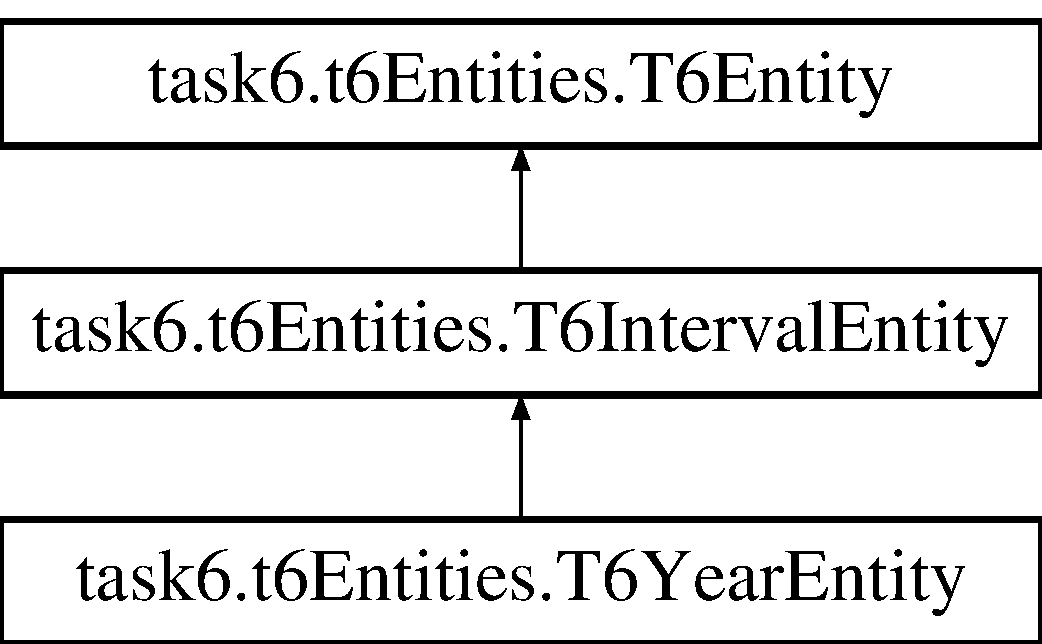
\includegraphics[height=3.000000cm]{classtask6_1_1t6Entities_1_1T6IntervalEntity}
\end{center}
\end{figure}
\subsection*{Public Member Functions}
\begin{DoxyCompactItemize}
\item 
def \hyperlink{classtask6_1_1t6Entities_1_1T6IntervalEntity_ac60a5e79fc1417b2447c865deeef4884}{\+\_\+\+\_\+init\+\_\+\+\_\+} (self, \hyperlink{classtask6_1_1t6Entities_1_1T6Entity_afeeced8134bb3ebe0cfecc64d0ab46a4}{id}, \hyperlink{classtask6_1_1t6Entities_1_1T6Entity_a52779e9af8864dc98e8b02fc5b9b041a}{start\+\_\+span}, \hyperlink{classtask6_1_1t6Entities_1_1T6Entity_aeb402200b156cd9562c5111dfe777b98}{end\+\_\+span}, \hyperlink{classtask6_1_1t6Entities_1_1T6Entity_ae4299399be3ecbd68dbb9ae988bff5a8}{type})
\end{DoxyCompactItemize}
\subsection*{Additional Inherited Members}


\subsection{Detailed Description}
An interval, just super classes for year interval for consistency. 

Definition at line 54 of file t6\+Entities.\+py.



\subsection{Constructor \& Destructor Documentation}
\mbox{\Hypertarget{classtask6_1_1t6Entities_1_1T6IntervalEntity_ac60a5e79fc1417b2447c865deeef4884}\label{classtask6_1_1t6Entities_1_1T6IntervalEntity_ac60a5e79fc1417b2447c865deeef4884}} 
\index{task6\+::t6\+Entities\+::\+T6\+Interval\+Entity@{task6\+::t6\+Entities\+::\+T6\+Interval\+Entity}!\+\_\+\+\_\+init\+\_\+\+\_\+@{\+\_\+\+\_\+init\+\_\+\+\_\+}}
\index{\+\_\+\+\_\+init\+\_\+\+\_\+@{\+\_\+\+\_\+init\+\_\+\+\_\+}!task6\+::t6\+Entities\+::\+T6\+Interval\+Entity@{task6\+::t6\+Entities\+::\+T6\+Interval\+Entity}}
\subsubsection{\texorpdfstring{\+\_\+\+\_\+init\+\_\+\+\_\+()}{\_\_init\_\_()}}
{\footnotesize\ttfamily def task6.\+t6\+Entities.\+T6\+Interval\+Entity.\+\_\+\+\_\+init\+\_\+\+\_\+ (\begin{DoxyParamCaption}\item[{}]{self,  }\item[{}]{id,  }\item[{}]{start\+\_\+span,  }\item[{}]{end\+\_\+span,  }\item[{}]{type }\end{DoxyParamCaption})}



Definition at line 55 of file t6\+Entities.\+py.



The documentation for this class was generated from the following file\+:\begin{DoxyCompactItemize}
\item 
task6/\hyperlink{t6Entities_8py}{t6\+Entities.\+py}\end{DoxyCompactItemize}

\hypertarget{classtask6_1_1t6Entities_1_1T6LastOperator}{}\section{task6.\+t6\+Entities.\+T6\+Last\+Operator Class Reference}
\label{classtask6_1_1t6Entities_1_1T6LastOperator}\index{task6.\+t6\+Entities.\+T6\+Last\+Operator@{task6.\+t6\+Entities.\+T6\+Last\+Operator}}


Create a last(\+Period) or last(Repeating-\/\+Interval) operator.  


Inheritance diagram for task6.\+t6\+Entities.\+T6\+Last\+Operator\+:\begin{figure}[H]
\begin{center}
\leavevmode
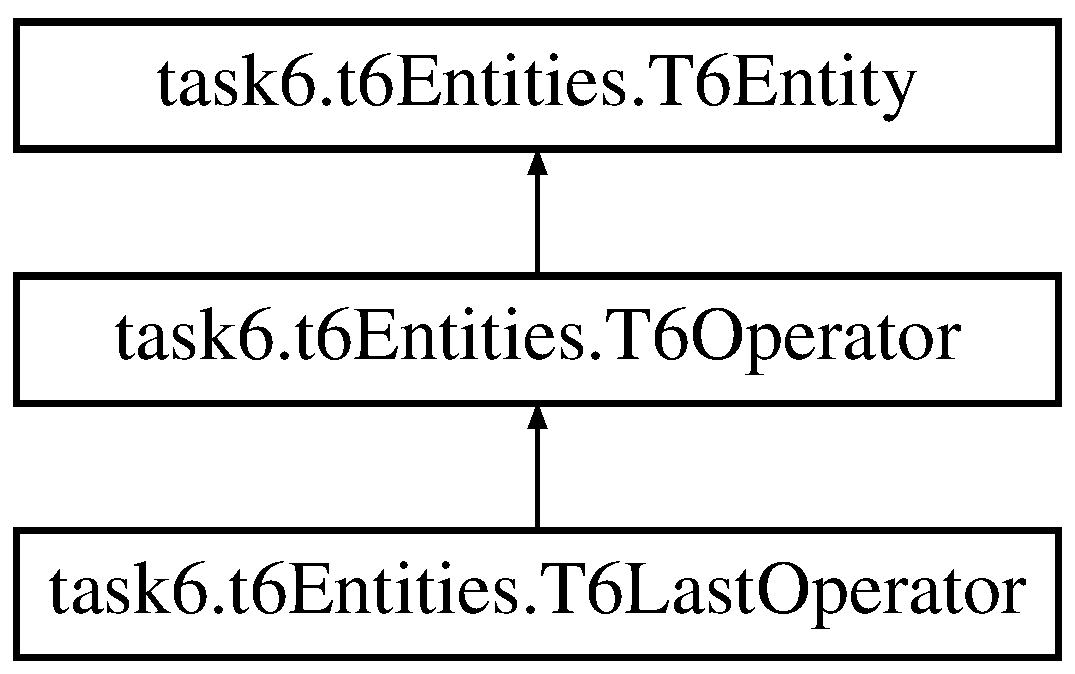
\includegraphics[height=3.000000cm]{classtask6_1_1t6Entities_1_1T6LastOperator}
\end{center}
\end{figure}
\subsection*{Public Member Functions}
\begin{DoxyCompactItemize}
\item 
def \hyperlink{classtask6_1_1t6Entities_1_1T6LastOperator_a16b9eca4b13c34d4615c7a654d30b501}{\+\_\+\+\_\+init\+\_\+\+\_\+} (self, \hyperlink{classtask6_1_1t6Entities_1_1T6Entity_afeeced8134bb3ebe0cfecc64d0ab46a4}{id}, \hyperlink{classtask6_1_1t6Entities_1_1T6Entity_a52779e9af8864dc98e8b02fc5b9b041a}{start\+\_\+span}, \hyperlink{classtask6_1_1t6Entities_1_1T6Entity_aeb402200b156cd9562c5111dfe777b98}{end\+\_\+span}, \hyperlink{classtask6_1_1t6Entities_1_1T6LastOperator_ace165f371e06ffdd35e81589f7e3ad4c}{semantics}, \hyperlink{classtask6_1_1t6Entities_1_1T6LastOperator_a5aeed327adbf129c1493d5782bd6afd4}{interval\+\_\+type}, \hyperlink{classtask6_1_1t6Entities_1_1T6LastOperator_aca10c8da0b6eea3185f66f103dca0a29}{interval}, \hyperlink{classtask6_1_1t6Entities_1_1T6LastOperator_ac165233979c84dfa138d76b67d171b1a}{period}, \hyperlink{classtask6_1_1t6Entities_1_1T6LastOperator_ab58d042c2aeff54eb56b7298375cb15b}{repeating\+\_\+interval})
\end{DoxyCompactItemize}
\subsection*{Public Attributes}
\begin{DoxyCompactItemize}
\item 
\hyperlink{classtask6_1_1t6Entities_1_1T6LastOperator_ace165f371e06ffdd35e81589f7e3ad4c}{semantics}
\item 
\hyperlink{classtask6_1_1t6Entities_1_1T6LastOperator_a5aeed327adbf129c1493d5782bd6afd4}{interval\+\_\+type}
\item 
\hyperlink{classtask6_1_1t6Entities_1_1T6LastOperator_aca10c8da0b6eea3185f66f103dca0a29}{interval}
\item 
\hyperlink{classtask6_1_1t6Entities_1_1T6LastOperator_ac165233979c84dfa138d76b67d171b1a}{period}
\item 
\hyperlink{classtask6_1_1t6Entities_1_1T6LastOperator_ab58d042c2aeff54eb56b7298375cb15b}{repeating\+\_\+interval}
\end{DoxyCompactItemize}


\subsection{Detailed Description}
Create a last(\+Period) or last(Repeating-\/\+Interval) operator. 


\begin{DoxyParams}{Parameters}
{\em semantics} & \{Interval-\/\+Included, Interval-\/\+Not-\/\+Included\} \\
\hline
\end{DoxyParams}


Definition at line 200 of file t6\+Entities.\+py.



\subsection{Constructor \& Destructor Documentation}
\mbox{\Hypertarget{classtask6_1_1t6Entities_1_1T6LastOperator_a16b9eca4b13c34d4615c7a654d30b501}\label{classtask6_1_1t6Entities_1_1T6LastOperator_a16b9eca4b13c34d4615c7a654d30b501}} 
\index{task6\+::t6\+Entities\+::\+T6\+Last\+Operator@{task6\+::t6\+Entities\+::\+T6\+Last\+Operator}!\+\_\+\+\_\+init\+\_\+\+\_\+@{\+\_\+\+\_\+init\+\_\+\+\_\+}}
\index{\+\_\+\+\_\+init\+\_\+\+\_\+@{\+\_\+\+\_\+init\+\_\+\+\_\+}!task6\+::t6\+Entities\+::\+T6\+Last\+Operator@{task6\+::t6\+Entities\+::\+T6\+Last\+Operator}}
\subsubsection{\texorpdfstring{\+\_\+\+\_\+init\+\_\+\+\_\+()}{\_\_init\_\_()}}
{\footnotesize\ttfamily def task6.\+t6\+Entities.\+T6\+Last\+Operator.\+\_\+\+\_\+init\+\_\+\+\_\+ (\begin{DoxyParamCaption}\item[{}]{self,  }\item[{}]{id,  }\item[{}]{start\+\_\+span,  }\item[{}]{end\+\_\+span,  }\item[{}]{semantics,  }\item[{}]{interval\+\_\+type,  }\item[{}]{interval,  }\item[{}]{period,  }\item[{}]{repeating\+\_\+interval }\end{DoxyParamCaption})}



Definition at line 201 of file t6\+Entities.\+py.



\subsection{Member Data Documentation}
\mbox{\Hypertarget{classtask6_1_1t6Entities_1_1T6LastOperator_aca10c8da0b6eea3185f66f103dca0a29}\label{classtask6_1_1t6Entities_1_1T6LastOperator_aca10c8da0b6eea3185f66f103dca0a29}} 
\index{task6\+::t6\+Entities\+::\+T6\+Last\+Operator@{task6\+::t6\+Entities\+::\+T6\+Last\+Operator}!interval@{interval}}
\index{interval@{interval}!task6\+::t6\+Entities\+::\+T6\+Last\+Operator@{task6\+::t6\+Entities\+::\+T6\+Last\+Operator}}
\subsubsection{\texorpdfstring{interval}{interval}}
{\footnotesize\ttfamily task6.\+t6\+Entities.\+T6\+Last\+Operator.\+interval}



Definition at line 205 of file t6\+Entities.\+py.

\mbox{\Hypertarget{classtask6_1_1t6Entities_1_1T6LastOperator_a5aeed327adbf129c1493d5782bd6afd4}\label{classtask6_1_1t6Entities_1_1T6LastOperator_a5aeed327adbf129c1493d5782bd6afd4}} 
\index{task6\+::t6\+Entities\+::\+T6\+Last\+Operator@{task6\+::t6\+Entities\+::\+T6\+Last\+Operator}!interval\+\_\+type@{interval\+\_\+type}}
\index{interval\+\_\+type@{interval\+\_\+type}!task6\+::t6\+Entities\+::\+T6\+Last\+Operator@{task6\+::t6\+Entities\+::\+T6\+Last\+Operator}}
\subsubsection{\texorpdfstring{interval\+\_\+type}{interval\_type}}
{\footnotesize\ttfamily task6.\+t6\+Entities.\+T6\+Last\+Operator.\+interval\+\_\+type}



Definition at line 204 of file t6\+Entities.\+py.

\mbox{\Hypertarget{classtask6_1_1t6Entities_1_1T6LastOperator_ac165233979c84dfa138d76b67d171b1a}\label{classtask6_1_1t6Entities_1_1T6LastOperator_ac165233979c84dfa138d76b67d171b1a}} 
\index{task6\+::t6\+Entities\+::\+T6\+Last\+Operator@{task6\+::t6\+Entities\+::\+T6\+Last\+Operator}!period@{period}}
\index{period@{period}!task6\+::t6\+Entities\+::\+T6\+Last\+Operator@{task6\+::t6\+Entities\+::\+T6\+Last\+Operator}}
\subsubsection{\texorpdfstring{period}{period}}
{\footnotesize\ttfamily task6.\+t6\+Entities.\+T6\+Last\+Operator.\+period}



Definition at line 206 of file t6\+Entities.\+py.

\mbox{\Hypertarget{classtask6_1_1t6Entities_1_1T6LastOperator_ab58d042c2aeff54eb56b7298375cb15b}\label{classtask6_1_1t6Entities_1_1T6LastOperator_ab58d042c2aeff54eb56b7298375cb15b}} 
\index{task6\+::t6\+Entities\+::\+T6\+Last\+Operator@{task6\+::t6\+Entities\+::\+T6\+Last\+Operator}!repeating\+\_\+interval@{repeating\+\_\+interval}}
\index{repeating\+\_\+interval@{repeating\+\_\+interval}!task6\+::t6\+Entities\+::\+T6\+Last\+Operator@{task6\+::t6\+Entities\+::\+T6\+Last\+Operator}}
\subsubsection{\texorpdfstring{repeating\+\_\+interval}{repeating\_interval}}
{\footnotesize\ttfamily task6.\+t6\+Entities.\+T6\+Last\+Operator.\+repeating\+\_\+interval}



Definition at line 207 of file t6\+Entities.\+py.

\mbox{\Hypertarget{classtask6_1_1t6Entities_1_1T6LastOperator_ace165f371e06ffdd35e81589f7e3ad4c}\label{classtask6_1_1t6Entities_1_1T6LastOperator_ace165f371e06ffdd35e81589f7e3ad4c}} 
\index{task6\+::t6\+Entities\+::\+T6\+Last\+Operator@{task6\+::t6\+Entities\+::\+T6\+Last\+Operator}!semantics@{semantics}}
\index{semantics@{semantics}!task6\+::t6\+Entities\+::\+T6\+Last\+Operator@{task6\+::t6\+Entities\+::\+T6\+Last\+Operator}}
\subsubsection{\texorpdfstring{semantics}{semantics}}
{\footnotesize\ttfamily task6.\+t6\+Entities.\+T6\+Last\+Operator.\+semantics}



Definition at line 203 of file t6\+Entities.\+py.



The documentation for this class was generated from the following file\+:\begin{DoxyCompactItemize}
\item 
task6/\hyperlink{t6Entities_8py}{t6\+Entities.\+py}\end{DoxyCompactItemize}

\hypertarget{classtask6_1_1t6Entities_1_1T6MinuteOfHourEntity}{}\section{task6.\+t6\+Entities.\+T6\+Minute\+Of\+Hour\+Entity Class Reference}
\label{classtask6_1_1t6Entities_1_1T6MinuteOfHourEntity}\index{task6.\+t6\+Entities.\+T6\+Minute\+Of\+Hour\+Entity@{task6.\+t6\+Entities.\+T6\+Minute\+Of\+Hour\+Entity}}
Inheritance diagram for task6.\+t6\+Entities.\+T6\+Minute\+Of\+Hour\+Entity\+:\begin{figure}[H]
\begin{center}
\leavevmode
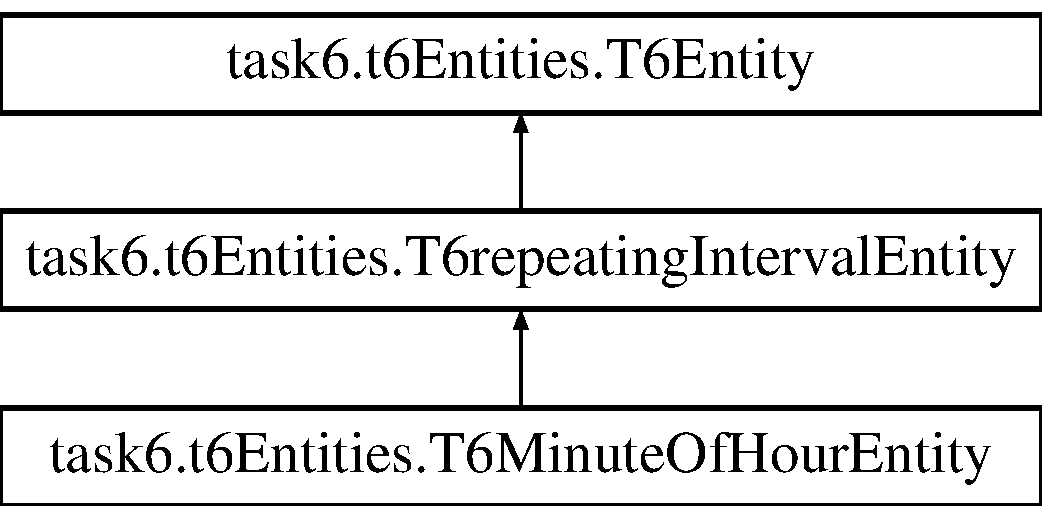
\includegraphics[height=3.000000cm]{classtask6_1_1t6Entities_1_1T6MinuteOfHourEntity}
\end{center}
\end{figure}
\subsection*{Public Member Functions}
\begin{DoxyCompactItemize}
\item 
def \hyperlink{classtask6_1_1t6Entities_1_1T6MinuteOfHourEntity_a927ef60688052a692beea14ebb684e2c}{\+\_\+\+\_\+init\+\_\+\+\_\+} (self, \hyperlink{classtask6_1_1t6Entities_1_1T6Entity_afeeced8134bb3ebe0cfecc64d0ab46a4}{id}, \hyperlink{classtask6_1_1t6Entities_1_1T6Entity_a52779e9af8864dc98e8b02fc5b9b041a}{start\+\_\+span}, \hyperlink{classtask6_1_1t6Entities_1_1T6Entity_aeb402200b156cd9562c5111dfe777b98}{end\+\_\+span}, \hyperlink{classtask6_1_1t6Entities_1_1T6MinuteOfHourEntity_abee1ba303976b6122dcf778c9e8763c6}{value}, \hyperlink{classtask6_1_1t6Entities_1_1T6MinuteOfHourEntity_a4c7879676d773211ec35ac3096b5d556}{sub\+\_\+interval}, \hyperlink{classtask6_1_1t6Entities_1_1T6MinuteOfHourEntity_a73b6e272b0a5092d03ddce3cf1745821}{number}, \hyperlink{classtask6_1_1t6Entities_1_1T6MinuteOfHourEntity_a1151c9a18ebeb805d6c8233f26d796b2}{modifier})
\end{DoxyCompactItemize}
\subsection*{Public Attributes}
\begin{DoxyCompactItemize}
\item 
\hyperlink{classtask6_1_1t6Entities_1_1T6MinuteOfHourEntity_abee1ba303976b6122dcf778c9e8763c6}{value}
\item 
\hyperlink{classtask6_1_1t6Entities_1_1T6MinuteOfHourEntity_a4c7879676d773211ec35ac3096b5d556}{sub\+\_\+interval}
\item 
\hyperlink{classtask6_1_1t6Entities_1_1T6MinuteOfHourEntity_a73b6e272b0a5092d03ddce3cf1745821}{number}
\item 
\hyperlink{classtask6_1_1t6Entities_1_1T6MinuteOfHourEntity_a1151c9a18ebeb805d6c8233f26d796b2}{modifier}
\end{DoxyCompactItemize}


\subsection{Detailed Description}


Definition at line 127 of file t6\+Entities.\+py.



\subsection{Constructor \& Destructor Documentation}
\mbox{\Hypertarget{classtask6_1_1t6Entities_1_1T6MinuteOfHourEntity_a927ef60688052a692beea14ebb684e2c}\label{classtask6_1_1t6Entities_1_1T6MinuteOfHourEntity_a927ef60688052a692beea14ebb684e2c}} 
\index{task6\+::t6\+Entities\+::\+T6\+Minute\+Of\+Hour\+Entity@{task6\+::t6\+Entities\+::\+T6\+Minute\+Of\+Hour\+Entity}!\+\_\+\+\_\+init\+\_\+\+\_\+@{\+\_\+\+\_\+init\+\_\+\+\_\+}}
\index{\+\_\+\+\_\+init\+\_\+\+\_\+@{\+\_\+\+\_\+init\+\_\+\+\_\+}!task6\+::t6\+Entities\+::\+T6\+Minute\+Of\+Hour\+Entity@{task6\+::t6\+Entities\+::\+T6\+Minute\+Of\+Hour\+Entity}}
\subsubsection{\texorpdfstring{\+\_\+\+\_\+init\+\_\+\+\_\+()}{\_\_init\_\_()}}
{\footnotesize\ttfamily def task6.\+t6\+Entities.\+T6\+Minute\+Of\+Hour\+Entity.\+\_\+\+\_\+init\+\_\+\+\_\+ (\begin{DoxyParamCaption}\item[{}]{self,  }\item[{}]{id,  }\item[{}]{start\+\_\+span,  }\item[{}]{end\+\_\+span,  }\item[{}]{value,  }\item[{}]{sub\+\_\+interval,  }\item[{}]{number,  }\item[{}]{modifier }\end{DoxyParamCaption})}



Definition at line 128 of file t6\+Entities.\+py.



\subsection{Member Data Documentation}
\mbox{\Hypertarget{classtask6_1_1t6Entities_1_1T6MinuteOfHourEntity_a1151c9a18ebeb805d6c8233f26d796b2}\label{classtask6_1_1t6Entities_1_1T6MinuteOfHourEntity_a1151c9a18ebeb805d6c8233f26d796b2}} 
\index{task6\+::t6\+Entities\+::\+T6\+Minute\+Of\+Hour\+Entity@{task6\+::t6\+Entities\+::\+T6\+Minute\+Of\+Hour\+Entity}!modifier@{modifier}}
\index{modifier@{modifier}!task6\+::t6\+Entities\+::\+T6\+Minute\+Of\+Hour\+Entity@{task6\+::t6\+Entities\+::\+T6\+Minute\+Of\+Hour\+Entity}}
\subsubsection{\texorpdfstring{modifier}{modifier}}
{\footnotesize\ttfamily task6.\+t6\+Entities.\+T6\+Minute\+Of\+Hour\+Entity.\+modifier}



Definition at line 133 of file t6\+Entities.\+py.

\mbox{\Hypertarget{classtask6_1_1t6Entities_1_1T6MinuteOfHourEntity_a73b6e272b0a5092d03ddce3cf1745821}\label{classtask6_1_1t6Entities_1_1T6MinuteOfHourEntity_a73b6e272b0a5092d03ddce3cf1745821}} 
\index{task6\+::t6\+Entities\+::\+T6\+Minute\+Of\+Hour\+Entity@{task6\+::t6\+Entities\+::\+T6\+Minute\+Of\+Hour\+Entity}!number@{number}}
\index{number@{number}!task6\+::t6\+Entities\+::\+T6\+Minute\+Of\+Hour\+Entity@{task6\+::t6\+Entities\+::\+T6\+Minute\+Of\+Hour\+Entity}}
\subsubsection{\texorpdfstring{number}{number}}
{\footnotesize\ttfamily task6.\+t6\+Entities.\+T6\+Minute\+Of\+Hour\+Entity.\+number}



Definition at line 132 of file t6\+Entities.\+py.

\mbox{\Hypertarget{classtask6_1_1t6Entities_1_1T6MinuteOfHourEntity_a4c7879676d773211ec35ac3096b5d556}\label{classtask6_1_1t6Entities_1_1T6MinuteOfHourEntity_a4c7879676d773211ec35ac3096b5d556}} 
\index{task6\+::t6\+Entities\+::\+T6\+Minute\+Of\+Hour\+Entity@{task6\+::t6\+Entities\+::\+T6\+Minute\+Of\+Hour\+Entity}!sub\+\_\+interval@{sub\+\_\+interval}}
\index{sub\+\_\+interval@{sub\+\_\+interval}!task6\+::t6\+Entities\+::\+T6\+Minute\+Of\+Hour\+Entity@{task6\+::t6\+Entities\+::\+T6\+Minute\+Of\+Hour\+Entity}}
\subsubsection{\texorpdfstring{sub\+\_\+interval}{sub\_interval}}
{\footnotesize\ttfamily task6.\+t6\+Entities.\+T6\+Minute\+Of\+Hour\+Entity.\+sub\+\_\+interval}



Definition at line 131 of file t6\+Entities.\+py.

\mbox{\Hypertarget{classtask6_1_1t6Entities_1_1T6MinuteOfHourEntity_abee1ba303976b6122dcf778c9e8763c6}\label{classtask6_1_1t6Entities_1_1T6MinuteOfHourEntity_abee1ba303976b6122dcf778c9e8763c6}} 
\index{task6\+::t6\+Entities\+::\+T6\+Minute\+Of\+Hour\+Entity@{task6\+::t6\+Entities\+::\+T6\+Minute\+Of\+Hour\+Entity}!value@{value}}
\index{value@{value}!task6\+::t6\+Entities\+::\+T6\+Minute\+Of\+Hour\+Entity@{task6\+::t6\+Entities\+::\+T6\+Minute\+Of\+Hour\+Entity}}
\subsubsection{\texorpdfstring{value}{value}}
{\footnotesize\ttfamily task6.\+t6\+Entities.\+T6\+Minute\+Of\+Hour\+Entity.\+value}



Definition at line 130 of file t6\+Entities.\+py.



The documentation for this class was generated from the following file\+:\begin{DoxyCompactItemize}
\item 
task6/\hyperlink{t6Entities_8py}{t6\+Entities.\+py}\end{DoxyCompactItemize}

\hypertarget{classtask6_1_1t6Entities_1_1T6Modifier}{}\section{task6.\+t6\+Entities.\+T6\+Modifier Class Reference}
\label{classtask6_1_1t6Entities_1_1T6Modifier}\index{task6.\+t6\+Entities.\+T6\+Modifier@{task6.\+t6\+Entities.\+T6\+Modifier}}
Inheritance diagram for task6.\+t6\+Entities.\+T6\+Modifier\+:\begin{figure}[H]
\begin{center}
\leavevmode
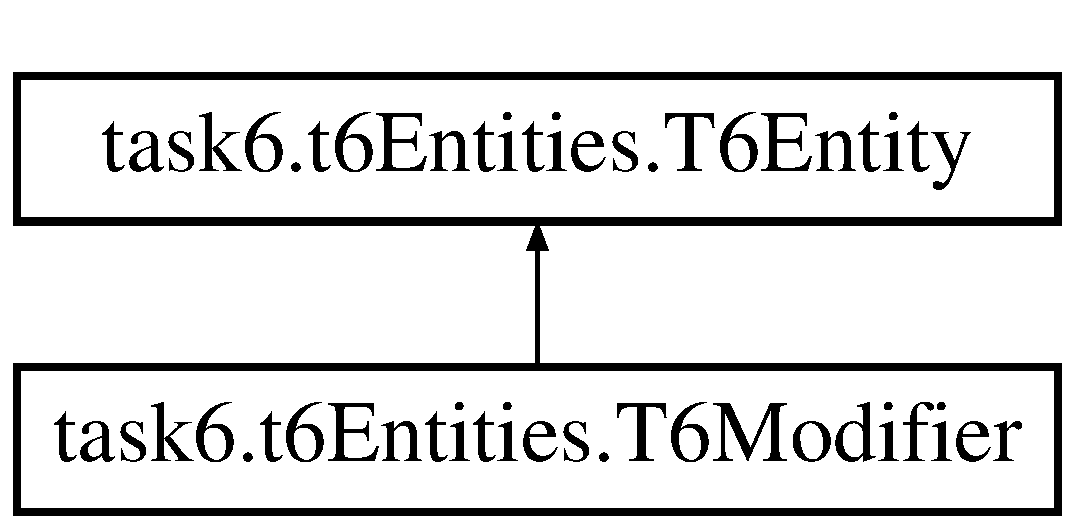
\includegraphics[height=2.000000cm]{classtask6_1_1t6Entities_1_1T6Modifier}
\end{center}
\end{figure}
\subsection*{Public Member Functions}
\begin{DoxyCompactItemize}
\item 
def \hyperlink{classtask6_1_1t6Entities_1_1T6Modifier_a472b7516cd488b8a12e8fff5ca48d1f5}{\+\_\+\+\_\+init\+\_\+\+\_\+} (self, \hyperlink{classtask6_1_1t6Entities_1_1T6Entity_afeeced8134bb3ebe0cfecc64d0ab46a4}{id}, \hyperlink{classtask6_1_1t6Entities_1_1T6Entity_a52779e9af8864dc98e8b02fc5b9b041a}{start\+\_\+span}, \hyperlink{classtask6_1_1t6Entities_1_1T6Entity_aeb402200b156cd9562c5111dfe777b98}{end\+\_\+span}, \hyperlink{classtask6_1_1t6Entities_1_1T6Modifier_adca8df4abb0ccb35146606b8610f27a1}{modifier})
\end{DoxyCompactItemize}
\subsection*{Public Attributes}
\begin{DoxyCompactItemize}
\item 
\hyperlink{classtask6_1_1t6Entities_1_1T6Modifier_adca8df4abb0ccb35146606b8610f27a1}{modifier}
\end{DoxyCompactItemize}


\subsection{Detailed Description}


Definition at line 272 of file t6\+Entities.\+py.



\subsection{Constructor \& Destructor Documentation}
\mbox{\Hypertarget{classtask6_1_1t6Entities_1_1T6Modifier_a472b7516cd488b8a12e8fff5ca48d1f5}\label{classtask6_1_1t6Entities_1_1T6Modifier_a472b7516cd488b8a12e8fff5ca48d1f5}} 
\index{task6\+::t6\+Entities\+::\+T6\+Modifier@{task6\+::t6\+Entities\+::\+T6\+Modifier}!\+\_\+\+\_\+init\+\_\+\+\_\+@{\+\_\+\+\_\+init\+\_\+\+\_\+}}
\index{\+\_\+\+\_\+init\+\_\+\+\_\+@{\+\_\+\+\_\+init\+\_\+\+\_\+}!task6\+::t6\+Entities\+::\+T6\+Modifier@{task6\+::t6\+Entities\+::\+T6\+Modifier}}
\subsubsection{\texorpdfstring{\+\_\+\+\_\+init\+\_\+\+\_\+()}{\_\_init\_\_()}}
{\footnotesize\ttfamily def task6.\+t6\+Entities.\+T6\+Modifier.\+\_\+\+\_\+init\+\_\+\+\_\+ (\begin{DoxyParamCaption}\item[{}]{self,  }\item[{}]{id,  }\item[{}]{start\+\_\+span,  }\item[{}]{end\+\_\+span,  }\item[{}]{modifier }\end{DoxyParamCaption})}



Definition at line 273 of file t6\+Entities.\+py.



\subsection{Member Data Documentation}
\mbox{\Hypertarget{classtask6_1_1t6Entities_1_1T6Modifier_adca8df4abb0ccb35146606b8610f27a1}\label{classtask6_1_1t6Entities_1_1T6Modifier_adca8df4abb0ccb35146606b8610f27a1}} 
\index{task6\+::t6\+Entities\+::\+T6\+Modifier@{task6\+::t6\+Entities\+::\+T6\+Modifier}!modifier@{modifier}}
\index{modifier@{modifier}!task6\+::t6\+Entities\+::\+T6\+Modifier@{task6\+::t6\+Entities\+::\+T6\+Modifier}}
\subsubsection{\texorpdfstring{modifier}{modifier}}
{\footnotesize\ttfamily task6.\+t6\+Entities.\+T6\+Modifier.\+modifier}



Definition at line 275 of file t6\+Entities.\+py.



The documentation for this class was generated from the following file\+:\begin{DoxyCompactItemize}
\item 
task6/\hyperlink{t6Entities_8py}{t6\+Entities.\+py}\end{DoxyCompactItemize}

\hypertarget{classtask6_1_1t6Entities_1_1T6MonthOfYearEntity}{}\section{task6.\+t6\+Entities.\+T6\+Month\+Of\+Year\+Entity Class Reference}
\label{classtask6_1_1t6Entities_1_1T6MonthOfYearEntity}\index{task6.\+t6\+Entities.\+T6\+Month\+Of\+Year\+Entity@{task6.\+t6\+Entities.\+T6\+Month\+Of\+Year\+Entity}}
Inheritance diagram for task6.\+t6\+Entities.\+T6\+Month\+Of\+Year\+Entity\+:\begin{figure}[H]
\begin{center}
\leavevmode
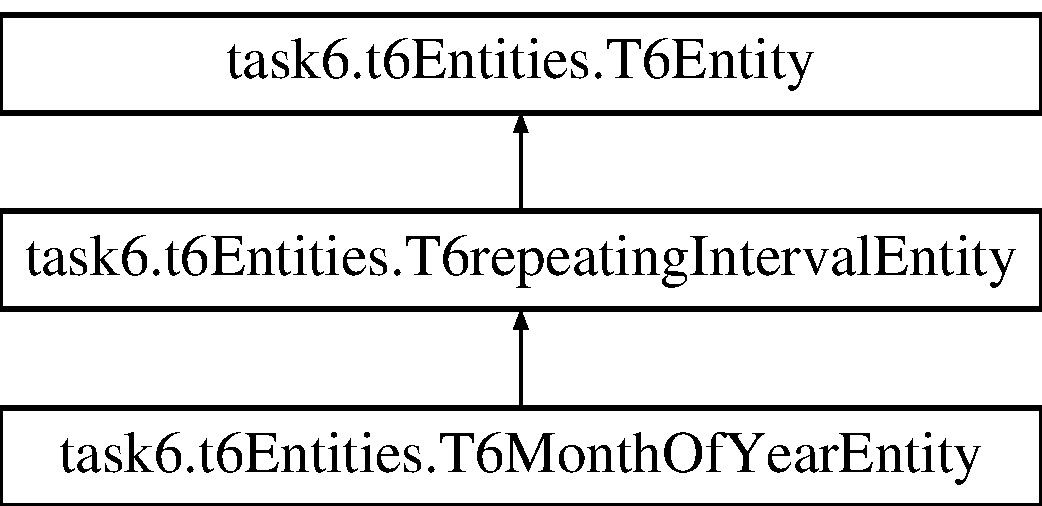
\includegraphics[height=3.000000cm]{classtask6_1_1t6Entities_1_1T6MonthOfYearEntity}
\end{center}
\end{figure}
\subsection*{Public Member Functions}
\begin{DoxyCompactItemize}
\item 
def \hyperlink{classtask6_1_1t6Entities_1_1T6MonthOfYearEntity_aafc8822d1941f3f61d379af1cc34fa59}{\+\_\+\+\_\+init\+\_\+\+\_\+} (self, \hyperlink{classtask6_1_1t6Entities_1_1T6Entity_afeeced8134bb3ebe0cfecc64d0ab46a4}{id}, \hyperlink{classtask6_1_1t6Entities_1_1T6Entity_a52779e9af8864dc98e8b02fc5b9b041a}{start\+\_\+span}, \hyperlink{classtask6_1_1t6Entities_1_1T6Entity_aeb402200b156cd9562c5111dfe777b98}{end\+\_\+span}, \hyperlink{classtask6_1_1t6Entities_1_1T6MonthOfYearEntity_a48a849892eb9cbc6fce3833f059989a7}{month\+\_\+type}, \hyperlink{classtask6_1_1t6Entities_1_1T6MonthOfYearEntity_ac2823d70e532c8032939f67a84c5efbc}{sub\+\_\+interval}, \hyperlink{classtask6_1_1t6Entities_1_1T6MonthOfYearEntity_a6b6c3d56962c165f446304d82d06acb0}{number}, \hyperlink{classtask6_1_1t6Entities_1_1T6MonthOfYearEntity_a1720393c88572b80a70fd30bbccea2ab}{modifier})
\end{DoxyCompactItemize}
\subsection*{Public Attributes}
\begin{DoxyCompactItemize}
\item 
\hyperlink{classtask6_1_1t6Entities_1_1T6MonthOfYearEntity_a48a849892eb9cbc6fce3833f059989a7}{month\+\_\+type}
\item 
\hyperlink{classtask6_1_1t6Entities_1_1T6MonthOfYearEntity_ac2823d70e532c8032939f67a84c5efbc}{sub\+\_\+interval}
\item 
\hyperlink{classtask6_1_1t6Entities_1_1T6MonthOfYearEntity_a6b6c3d56962c165f446304d82d06acb0}{number}
\item 
\hyperlink{classtask6_1_1t6Entities_1_1T6MonthOfYearEntity_a1720393c88572b80a70fd30bbccea2ab}{modifier}
\end{DoxyCompactItemize}


\subsection{Detailed Description}


Definition at line 86 of file t6\+Entities.\+py.



\subsection{Constructor \& Destructor Documentation}
\mbox{\Hypertarget{classtask6_1_1t6Entities_1_1T6MonthOfYearEntity_aafc8822d1941f3f61d379af1cc34fa59}\label{classtask6_1_1t6Entities_1_1T6MonthOfYearEntity_aafc8822d1941f3f61d379af1cc34fa59}} 
\index{task6\+::t6\+Entities\+::\+T6\+Month\+Of\+Year\+Entity@{task6\+::t6\+Entities\+::\+T6\+Month\+Of\+Year\+Entity}!\+\_\+\+\_\+init\+\_\+\+\_\+@{\+\_\+\+\_\+init\+\_\+\+\_\+}}
\index{\+\_\+\+\_\+init\+\_\+\+\_\+@{\+\_\+\+\_\+init\+\_\+\+\_\+}!task6\+::t6\+Entities\+::\+T6\+Month\+Of\+Year\+Entity@{task6\+::t6\+Entities\+::\+T6\+Month\+Of\+Year\+Entity}}
\subsubsection{\texorpdfstring{\+\_\+\+\_\+init\+\_\+\+\_\+()}{\_\_init\_\_()}}
{\footnotesize\ttfamily def task6.\+t6\+Entities.\+T6\+Month\+Of\+Year\+Entity.\+\_\+\+\_\+init\+\_\+\+\_\+ (\begin{DoxyParamCaption}\item[{}]{self,  }\item[{}]{id,  }\item[{}]{start\+\_\+span,  }\item[{}]{end\+\_\+span,  }\item[{}]{month\+\_\+type,  }\item[{}]{sub\+\_\+interval,  }\item[{}]{number,  }\item[{}]{modifier }\end{DoxyParamCaption})}



Definition at line 87 of file t6\+Entities.\+py.



\subsection{Member Data Documentation}
\mbox{\Hypertarget{classtask6_1_1t6Entities_1_1T6MonthOfYearEntity_a1720393c88572b80a70fd30bbccea2ab}\label{classtask6_1_1t6Entities_1_1T6MonthOfYearEntity_a1720393c88572b80a70fd30bbccea2ab}} 
\index{task6\+::t6\+Entities\+::\+T6\+Month\+Of\+Year\+Entity@{task6\+::t6\+Entities\+::\+T6\+Month\+Of\+Year\+Entity}!modifier@{modifier}}
\index{modifier@{modifier}!task6\+::t6\+Entities\+::\+T6\+Month\+Of\+Year\+Entity@{task6\+::t6\+Entities\+::\+T6\+Month\+Of\+Year\+Entity}}
\subsubsection{\texorpdfstring{modifier}{modifier}}
{\footnotesize\ttfamily task6.\+t6\+Entities.\+T6\+Month\+Of\+Year\+Entity.\+modifier}



Definition at line 92 of file t6\+Entities.\+py.

\mbox{\Hypertarget{classtask6_1_1t6Entities_1_1T6MonthOfYearEntity_a48a849892eb9cbc6fce3833f059989a7}\label{classtask6_1_1t6Entities_1_1T6MonthOfYearEntity_a48a849892eb9cbc6fce3833f059989a7}} 
\index{task6\+::t6\+Entities\+::\+T6\+Month\+Of\+Year\+Entity@{task6\+::t6\+Entities\+::\+T6\+Month\+Of\+Year\+Entity}!month\+\_\+type@{month\+\_\+type}}
\index{month\+\_\+type@{month\+\_\+type}!task6\+::t6\+Entities\+::\+T6\+Month\+Of\+Year\+Entity@{task6\+::t6\+Entities\+::\+T6\+Month\+Of\+Year\+Entity}}
\subsubsection{\texorpdfstring{month\+\_\+type}{month\_type}}
{\footnotesize\ttfamily task6.\+t6\+Entities.\+T6\+Month\+Of\+Year\+Entity.\+month\+\_\+type}



Definition at line 89 of file t6\+Entities.\+py.

\mbox{\Hypertarget{classtask6_1_1t6Entities_1_1T6MonthOfYearEntity_a6b6c3d56962c165f446304d82d06acb0}\label{classtask6_1_1t6Entities_1_1T6MonthOfYearEntity_a6b6c3d56962c165f446304d82d06acb0}} 
\index{task6\+::t6\+Entities\+::\+T6\+Month\+Of\+Year\+Entity@{task6\+::t6\+Entities\+::\+T6\+Month\+Of\+Year\+Entity}!number@{number}}
\index{number@{number}!task6\+::t6\+Entities\+::\+T6\+Month\+Of\+Year\+Entity@{task6\+::t6\+Entities\+::\+T6\+Month\+Of\+Year\+Entity}}
\subsubsection{\texorpdfstring{number}{number}}
{\footnotesize\ttfamily task6.\+t6\+Entities.\+T6\+Month\+Of\+Year\+Entity.\+number}



Definition at line 91 of file t6\+Entities.\+py.

\mbox{\Hypertarget{classtask6_1_1t6Entities_1_1T6MonthOfYearEntity_ac2823d70e532c8032939f67a84c5efbc}\label{classtask6_1_1t6Entities_1_1T6MonthOfYearEntity_ac2823d70e532c8032939f67a84c5efbc}} 
\index{task6\+::t6\+Entities\+::\+T6\+Month\+Of\+Year\+Entity@{task6\+::t6\+Entities\+::\+T6\+Month\+Of\+Year\+Entity}!sub\+\_\+interval@{sub\+\_\+interval}}
\index{sub\+\_\+interval@{sub\+\_\+interval}!task6\+::t6\+Entities\+::\+T6\+Month\+Of\+Year\+Entity@{task6\+::t6\+Entities\+::\+T6\+Month\+Of\+Year\+Entity}}
\subsubsection{\texorpdfstring{sub\+\_\+interval}{sub\_interval}}
{\footnotesize\ttfamily task6.\+t6\+Entities.\+T6\+Month\+Of\+Year\+Entity.\+sub\+\_\+interval}



Definition at line 90 of file t6\+Entities.\+py.



The documentation for this class was generated from the following file\+:\begin{DoxyCompactItemize}
\item 
task6/\hyperlink{t6Entities_8py}{t6\+Entities.\+py}\end{DoxyCompactItemize}

\hypertarget{classtask6_1_1t6Entities_1_1T6NextOperator}{}\section{task6.\+t6\+Entities.\+T6\+Next\+Operator Class Reference}
\label{classtask6_1_1t6Entities_1_1T6NextOperator}\index{task6.\+t6\+Entities.\+T6\+Next\+Operator@{task6.\+t6\+Entities.\+T6\+Next\+Operator}}
Inheritance diagram for task6.\+t6\+Entities.\+T6\+Next\+Operator\+:\begin{figure}[H]
\begin{center}
\leavevmode
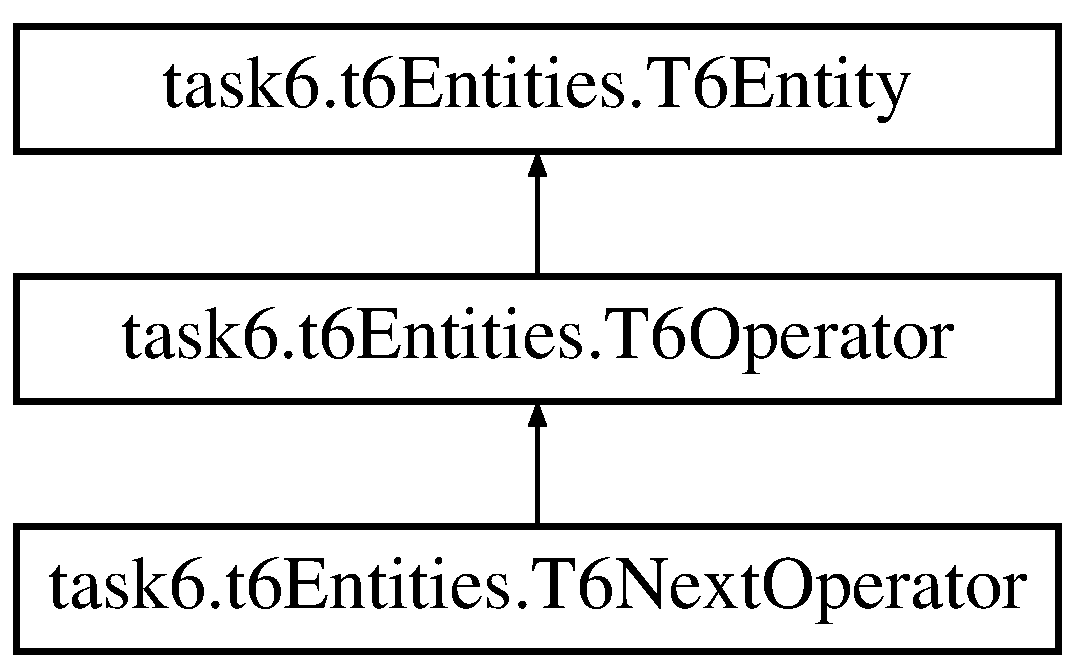
\includegraphics[height=3.000000cm]{classtask6_1_1t6Entities_1_1T6NextOperator}
\end{center}
\end{figure}
\subsection*{Public Member Functions}
\begin{DoxyCompactItemize}
\item 
def \hyperlink{classtask6_1_1t6Entities_1_1T6NextOperator_a52ca482e1fb78073e0bfaa804558846d}{\+\_\+\+\_\+init\+\_\+\+\_\+} (self, \hyperlink{classtask6_1_1t6Entities_1_1T6Entity_afeeced8134bb3ebe0cfecc64d0ab46a4}{id}, \hyperlink{classtask6_1_1t6Entities_1_1T6Entity_a52779e9af8864dc98e8b02fc5b9b041a}{start\+\_\+span}, \hyperlink{classtask6_1_1t6Entities_1_1T6Entity_aeb402200b156cd9562c5111dfe777b98}{end\+\_\+span}, \hyperlink{classtask6_1_1t6Entities_1_1T6NextOperator_a28e1b4345fea8b5436687c45d6daf2a9}{interval\+\_\+type}, \hyperlink{classtask6_1_1t6Entities_1_1T6NextOperator_a4059079dc037d178dbda878e60051ba0}{interval}, \hyperlink{classtask6_1_1t6Entities_1_1T6NextOperator_acc493ea5fb1baf65832d630812ae7299}{period}, \hyperlink{classtask6_1_1t6Entities_1_1T6NextOperator_a66a96468dd1b550691e461d897c05c99}{repeating\+\_\+interval}, \hyperlink{classtask6_1_1t6Entities_1_1T6NextOperator_a2d4bc12cdc90894fb48afc39adb4ffab}{semantics})
\end{DoxyCompactItemize}
\subsection*{Public Attributes}
\begin{DoxyCompactItemize}
\item 
\hyperlink{classtask6_1_1t6Entities_1_1T6NextOperator_a28e1b4345fea8b5436687c45d6daf2a9}{interval\+\_\+type}
\item 
\hyperlink{classtask6_1_1t6Entities_1_1T6NextOperator_a4059079dc037d178dbda878e60051ba0}{interval}
\item 
\hyperlink{classtask6_1_1t6Entities_1_1T6NextOperator_acc493ea5fb1baf65832d630812ae7299}{period}
\item 
\hyperlink{classtask6_1_1t6Entities_1_1T6NextOperator_a66a96468dd1b550691e461d897c05c99}{repeating\+\_\+interval}
\item 
\hyperlink{classtask6_1_1t6Entities_1_1T6NextOperator_a2d4bc12cdc90894fb48afc39adb4ffab}{semantics}
\end{DoxyCompactItemize}


\subsection{Detailed Description}


Definition at line 209 of file t6\+Entities.\+py.



\subsection{Constructor \& Destructor Documentation}
\mbox{\Hypertarget{classtask6_1_1t6Entities_1_1T6NextOperator_a52ca482e1fb78073e0bfaa804558846d}\label{classtask6_1_1t6Entities_1_1T6NextOperator_a52ca482e1fb78073e0bfaa804558846d}} 
\index{task6\+::t6\+Entities\+::\+T6\+Next\+Operator@{task6\+::t6\+Entities\+::\+T6\+Next\+Operator}!\+\_\+\+\_\+init\+\_\+\+\_\+@{\+\_\+\+\_\+init\+\_\+\+\_\+}}
\index{\+\_\+\+\_\+init\+\_\+\+\_\+@{\+\_\+\+\_\+init\+\_\+\+\_\+}!task6\+::t6\+Entities\+::\+T6\+Next\+Operator@{task6\+::t6\+Entities\+::\+T6\+Next\+Operator}}
\subsubsection{\texorpdfstring{\+\_\+\+\_\+init\+\_\+\+\_\+()}{\_\_init\_\_()}}
{\footnotesize\ttfamily def task6.\+t6\+Entities.\+T6\+Next\+Operator.\+\_\+\+\_\+init\+\_\+\+\_\+ (\begin{DoxyParamCaption}\item[{}]{self,  }\item[{}]{id,  }\item[{}]{start\+\_\+span,  }\item[{}]{end\+\_\+span,  }\item[{}]{interval\+\_\+type,  }\item[{}]{interval,  }\item[{}]{period,  }\item[{}]{repeating\+\_\+interval,  }\item[{}]{semantics }\end{DoxyParamCaption})}



Definition at line 210 of file t6\+Entities.\+py.



\subsection{Member Data Documentation}
\mbox{\Hypertarget{classtask6_1_1t6Entities_1_1T6NextOperator_a4059079dc037d178dbda878e60051ba0}\label{classtask6_1_1t6Entities_1_1T6NextOperator_a4059079dc037d178dbda878e60051ba0}} 
\index{task6\+::t6\+Entities\+::\+T6\+Next\+Operator@{task6\+::t6\+Entities\+::\+T6\+Next\+Operator}!interval@{interval}}
\index{interval@{interval}!task6\+::t6\+Entities\+::\+T6\+Next\+Operator@{task6\+::t6\+Entities\+::\+T6\+Next\+Operator}}
\subsubsection{\texorpdfstring{interval}{interval}}
{\footnotesize\ttfamily task6.\+t6\+Entities.\+T6\+Next\+Operator.\+interval}



Definition at line 213 of file t6\+Entities.\+py.

\mbox{\Hypertarget{classtask6_1_1t6Entities_1_1T6NextOperator_a28e1b4345fea8b5436687c45d6daf2a9}\label{classtask6_1_1t6Entities_1_1T6NextOperator_a28e1b4345fea8b5436687c45d6daf2a9}} 
\index{task6\+::t6\+Entities\+::\+T6\+Next\+Operator@{task6\+::t6\+Entities\+::\+T6\+Next\+Operator}!interval\+\_\+type@{interval\+\_\+type}}
\index{interval\+\_\+type@{interval\+\_\+type}!task6\+::t6\+Entities\+::\+T6\+Next\+Operator@{task6\+::t6\+Entities\+::\+T6\+Next\+Operator}}
\subsubsection{\texorpdfstring{interval\+\_\+type}{interval\_type}}
{\footnotesize\ttfamily task6.\+t6\+Entities.\+T6\+Next\+Operator.\+interval\+\_\+type}



Definition at line 212 of file t6\+Entities.\+py.

\mbox{\Hypertarget{classtask6_1_1t6Entities_1_1T6NextOperator_acc493ea5fb1baf65832d630812ae7299}\label{classtask6_1_1t6Entities_1_1T6NextOperator_acc493ea5fb1baf65832d630812ae7299}} 
\index{task6\+::t6\+Entities\+::\+T6\+Next\+Operator@{task6\+::t6\+Entities\+::\+T6\+Next\+Operator}!period@{period}}
\index{period@{period}!task6\+::t6\+Entities\+::\+T6\+Next\+Operator@{task6\+::t6\+Entities\+::\+T6\+Next\+Operator}}
\subsubsection{\texorpdfstring{period}{period}}
{\footnotesize\ttfamily task6.\+t6\+Entities.\+T6\+Next\+Operator.\+period}



Definition at line 214 of file t6\+Entities.\+py.

\mbox{\Hypertarget{classtask6_1_1t6Entities_1_1T6NextOperator_a66a96468dd1b550691e461d897c05c99}\label{classtask6_1_1t6Entities_1_1T6NextOperator_a66a96468dd1b550691e461d897c05c99}} 
\index{task6\+::t6\+Entities\+::\+T6\+Next\+Operator@{task6\+::t6\+Entities\+::\+T6\+Next\+Operator}!repeating\+\_\+interval@{repeating\+\_\+interval}}
\index{repeating\+\_\+interval@{repeating\+\_\+interval}!task6\+::t6\+Entities\+::\+T6\+Next\+Operator@{task6\+::t6\+Entities\+::\+T6\+Next\+Operator}}
\subsubsection{\texorpdfstring{repeating\+\_\+interval}{repeating\_interval}}
{\footnotesize\ttfamily task6.\+t6\+Entities.\+T6\+Next\+Operator.\+repeating\+\_\+interval}



Definition at line 215 of file t6\+Entities.\+py.

\mbox{\Hypertarget{classtask6_1_1t6Entities_1_1T6NextOperator_a2d4bc12cdc90894fb48afc39adb4ffab}\label{classtask6_1_1t6Entities_1_1T6NextOperator_a2d4bc12cdc90894fb48afc39adb4ffab}} 
\index{task6\+::t6\+Entities\+::\+T6\+Next\+Operator@{task6\+::t6\+Entities\+::\+T6\+Next\+Operator}!semantics@{semantics}}
\index{semantics@{semantics}!task6\+::t6\+Entities\+::\+T6\+Next\+Operator@{task6\+::t6\+Entities\+::\+T6\+Next\+Operator}}
\subsubsection{\texorpdfstring{semantics}{semantics}}
{\footnotesize\ttfamily task6.\+t6\+Entities.\+T6\+Next\+Operator.\+semantics}



Definition at line 216 of file t6\+Entities.\+py.



The documentation for this class was generated from the following file\+:\begin{DoxyCompactItemize}
\item 
task6/\hyperlink{t6Entities_8py}{t6\+Entities.\+py}\end{DoxyCompactItemize}

\hypertarget{classtask6_1_1t6Entities_1_1T6NthOperator}{}\section{task6.\+t6\+Entities.\+T6\+Nth\+Operator Class Reference}
\label{classtask6_1_1t6Entities_1_1T6NthOperator}\index{task6.\+t6\+Entities.\+T6\+Nth\+Operator@{task6.\+t6\+Entities.\+T6\+Nth\+Operator}}
Inheritance diagram for task6.\+t6\+Entities.\+T6\+Nth\+Operator\+:\begin{figure}[H]
\begin{center}
\leavevmode
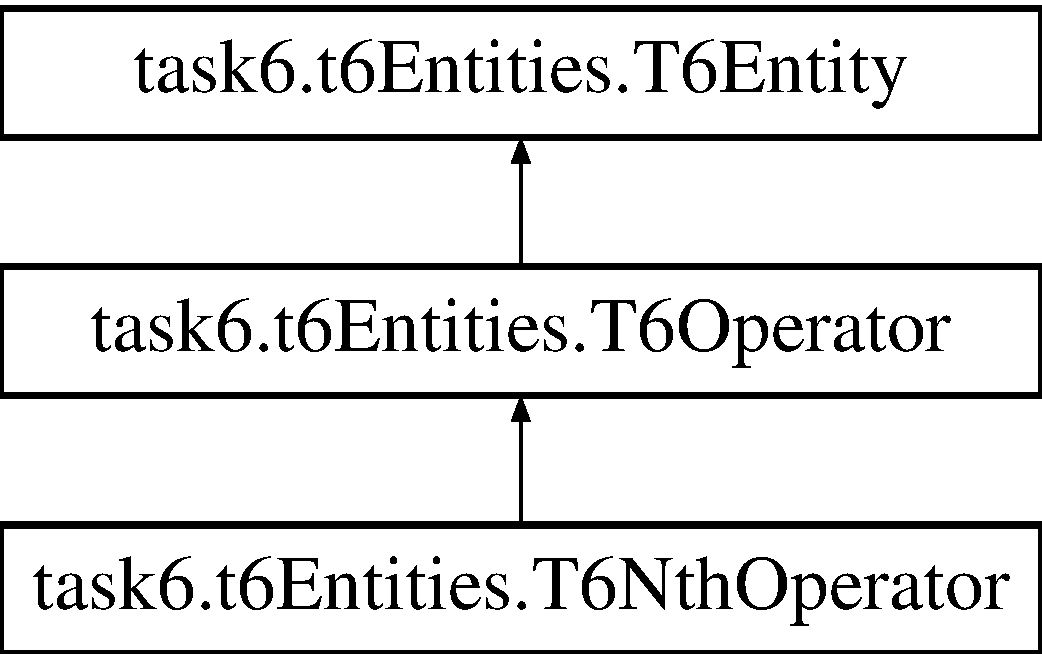
\includegraphics[height=3.000000cm]{classtask6_1_1t6Entities_1_1T6NthOperator}
\end{center}
\end{figure}
\subsection*{Public Member Functions}
\begin{DoxyCompactItemize}
\item 
def \hyperlink{classtask6_1_1t6Entities_1_1T6NthOperator_a8233039b4503d58bb61f2a81c9e5ab8a}{\+\_\+\+\_\+init\+\_\+\+\_\+} (self, \hyperlink{classtask6_1_1t6Entities_1_1T6Entity_afeeced8134bb3ebe0cfecc64d0ab46a4}{id}, \hyperlink{classtask6_1_1t6Entities_1_1T6Entity_a52779e9af8864dc98e8b02fc5b9b041a}{start\+\_\+span}, \hyperlink{classtask6_1_1t6Entities_1_1T6Entity_aeb402200b156cd9562c5111dfe777b98}{end\+\_\+span}, \hyperlink{classtask6_1_1t6Entities_1_1T6NthOperator_ae675666c1fa8791ff44ffe276eb28c9e}{interval\+\_\+type}, \hyperlink{classtask6_1_1t6Entities_1_1T6NthOperator_a2482a1dd907a4d625dd56645b2fae789}{interval}, \hyperlink{classtask6_1_1t6Entities_1_1T6NthOperator_aa330004bf54b51adec750472236e60ed}{period}, \hyperlink{classtask6_1_1t6Entities_1_1T6NthOperator_a02427933a75c637d8eae20e00cec6bfd}{repeating\+\_\+interval})
\end{DoxyCompactItemize}
\subsection*{Public Attributes}
\begin{DoxyCompactItemize}
\item 
\hyperlink{classtask6_1_1t6Entities_1_1T6NthOperator_ae675666c1fa8791ff44ffe276eb28c9e}{interval\+\_\+type}
\item 
\hyperlink{classtask6_1_1t6Entities_1_1T6NthOperator_a2482a1dd907a4d625dd56645b2fae789}{interval}
\item 
\hyperlink{classtask6_1_1t6Entities_1_1T6NthOperator_aa330004bf54b51adec750472236e60ed}{period}
\item 
\hyperlink{classtask6_1_1t6Entities_1_1T6NthOperator_a02427933a75c637d8eae20e00cec6bfd}{repeating\+\_\+interval}
\end{DoxyCompactItemize}


\subsection{Detailed Description}


Definition at line 251 of file t6\+Entities.\+py.



\subsection{Constructor \& Destructor Documentation}
\mbox{\Hypertarget{classtask6_1_1t6Entities_1_1T6NthOperator_a8233039b4503d58bb61f2a81c9e5ab8a}\label{classtask6_1_1t6Entities_1_1T6NthOperator_a8233039b4503d58bb61f2a81c9e5ab8a}} 
\index{task6\+::t6\+Entities\+::\+T6\+Nth\+Operator@{task6\+::t6\+Entities\+::\+T6\+Nth\+Operator}!\+\_\+\+\_\+init\+\_\+\+\_\+@{\+\_\+\+\_\+init\+\_\+\+\_\+}}
\index{\+\_\+\+\_\+init\+\_\+\+\_\+@{\+\_\+\+\_\+init\+\_\+\+\_\+}!task6\+::t6\+Entities\+::\+T6\+Nth\+Operator@{task6\+::t6\+Entities\+::\+T6\+Nth\+Operator}}
\subsubsection{\texorpdfstring{\+\_\+\+\_\+init\+\_\+\+\_\+()}{\_\_init\_\_()}}
{\footnotesize\ttfamily def task6.\+t6\+Entities.\+T6\+Nth\+Operator.\+\_\+\+\_\+init\+\_\+\+\_\+ (\begin{DoxyParamCaption}\item[{}]{self,  }\item[{}]{id,  }\item[{}]{start\+\_\+span,  }\item[{}]{end\+\_\+span,  }\item[{}]{interval\+\_\+type,  }\item[{}]{interval,  }\item[{}]{period,  }\item[{}]{repeating\+\_\+interval }\end{DoxyParamCaption})}



Definition at line 252 of file t6\+Entities.\+py.



\subsection{Member Data Documentation}
\mbox{\Hypertarget{classtask6_1_1t6Entities_1_1T6NthOperator_a2482a1dd907a4d625dd56645b2fae789}\label{classtask6_1_1t6Entities_1_1T6NthOperator_a2482a1dd907a4d625dd56645b2fae789}} 
\index{task6\+::t6\+Entities\+::\+T6\+Nth\+Operator@{task6\+::t6\+Entities\+::\+T6\+Nth\+Operator}!interval@{interval}}
\index{interval@{interval}!task6\+::t6\+Entities\+::\+T6\+Nth\+Operator@{task6\+::t6\+Entities\+::\+T6\+Nth\+Operator}}
\subsubsection{\texorpdfstring{interval}{interval}}
{\footnotesize\ttfamily task6.\+t6\+Entities.\+T6\+Nth\+Operator.\+interval}



Definition at line 255 of file t6\+Entities.\+py.

\mbox{\Hypertarget{classtask6_1_1t6Entities_1_1T6NthOperator_ae675666c1fa8791ff44ffe276eb28c9e}\label{classtask6_1_1t6Entities_1_1T6NthOperator_ae675666c1fa8791ff44ffe276eb28c9e}} 
\index{task6\+::t6\+Entities\+::\+T6\+Nth\+Operator@{task6\+::t6\+Entities\+::\+T6\+Nth\+Operator}!interval\+\_\+type@{interval\+\_\+type}}
\index{interval\+\_\+type@{interval\+\_\+type}!task6\+::t6\+Entities\+::\+T6\+Nth\+Operator@{task6\+::t6\+Entities\+::\+T6\+Nth\+Operator}}
\subsubsection{\texorpdfstring{interval\+\_\+type}{interval\_type}}
{\footnotesize\ttfamily task6.\+t6\+Entities.\+T6\+Nth\+Operator.\+interval\+\_\+type}



Definition at line 254 of file t6\+Entities.\+py.

\mbox{\Hypertarget{classtask6_1_1t6Entities_1_1T6NthOperator_aa330004bf54b51adec750472236e60ed}\label{classtask6_1_1t6Entities_1_1T6NthOperator_aa330004bf54b51adec750472236e60ed}} 
\index{task6\+::t6\+Entities\+::\+T6\+Nth\+Operator@{task6\+::t6\+Entities\+::\+T6\+Nth\+Operator}!period@{period}}
\index{period@{period}!task6\+::t6\+Entities\+::\+T6\+Nth\+Operator@{task6\+::t6\+Entities\+::\+T6\+Nth\+Operator}}
\subsubsection{\texorpdfstring{period}{period}}
{\footnotesize\ttfamily task6.\+t6\+Entities.\+T6\+Nth\+Operator.\+period}



Definition at line 256 of file t6\+Entities.\+py.

\mbox{\Hypertarget{classtask6_1_1t6Entities_1_1T6NthOperator_a02427933a75c637d8eae20e00cec6bfd}\label{classtask6_1_1t6Entities_1_1T6NthOperator_a02427933a75c637d8eae20e00cec6bfd}} 
\index{task6\+::t6\+Entities\+::\+T6\+Nth\+Operator@{task6\+::t6\+Entities\+::\+T6\+Nth\+Operator}!repeating\+\_\+interval@{repeating\+\_\+interval}}
\index{repeating\+\_\+interval@{repeating\+\_\+interval}!task6\+::t6\+Entities\+::\+T6\+Nth\+Operator@{task6\+::t6\+Entities\+::\+T6\+Nth\+Operator}}
\subsubsection{\texorpdfstring{repeating\+\_\+interval}{repeating\_interval}}
{\footnotesize\ttfamily task6.\+t6\+Entities.\+T6\+Nth\+Operator.\+repeating\+\_\+interval}



Definition at line 257 of file t6\+Entities.\+py.



The documentation for this class was generated from the following file\+:\begin{DoxyCompactItemize}
\item 
task6/\hyperlink{t6Entities_8py}{t6\+Entities.\+py}\end{DoxyCompactItemize}

\hypertarget{classtask6_1_1t6Entities_1_1T6Number}{}\section{task6.\+t6\+Entities.\+T6\+Number Class Reference}
\label{classtask6_1_1t6Entities_1_1T6Number}\index{task6.\+t6\+Entities.\+T6\+Number@{task6.\+t6\+Entities.\+T6\+Number}}
Inheritance diagram for task6.\+t6\+Entities.\+T6\+Number\+:\begin{figure}[H]
\begin{center}
\leavevmode
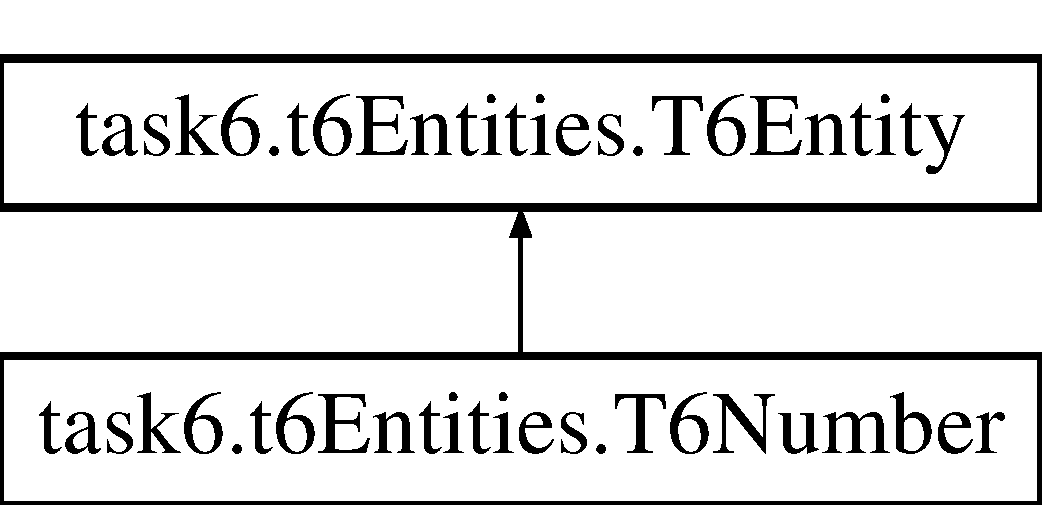
\includegraphics[height=2.000000cm]{classtask6_1_1t6Entities_1_1T6Number}
\end{center}
\end{figure}
\subsection*{Public Member Functions}
\begin{DoxyCompactItemize}
\item 
def \hyperlink{classtask6_1_1t6Entities_1_1T6Number_a1b851deb36620e06ae15585568f49cc3}{\+\_\+\+\_\+init\+\_\+\+\_\+} (self, \hyperlink{classtask6_1_1t6Entities_1_1T6Entity_afeeced8134bb3ebe0cfecc64d0ab46a4}{id}, \hyperlink{classtask6_1_1t6Entities_1_1T6Entity_a52779e9af8864dc98e8b02fc5b9b041a}{start\+\_\+span}, \hyperlink{classtask6_1_1t6Entities_1_1T6Entity_aeb402200b156cd9562c5111dfe777b98}{end\+\_\+span}, \hyperlink{classtask6_1_1t6Entities_1_1T6Number_a0a09fb41791cdfb13680185e7d996d8c}{value})
\end{DoxyCompactItemize}
\subsection*{Public Attributes}
\begin{DoxyCompactItemize}
\item 
\hyperlink{classtask6_1_1t6Entities_1_1T6Number_a0a09fb41791cdfb13680185e7d996d8c}{value}
\end{DoxyCompactItemize}


\subsection{Detailed Description}


Definition at line 267 of file t6\+Entities.\+py.



\subsection{Constructor \& Destructor Documentation}
\mbox{\Hypertarget{classtask6_1_1t6Entities_1_1T6Number_a1b851deb36620e06ae15585568f49cc3}\label{classtask6_1_1t6Entities_1_1T6Number_a1b851deb36620e06ae15585568f49cc3}} 
\index{task6\+::t6\+Entities\+::\+T6\+Number@{task6\+::t6\+Entities\+::\+T6\+Number}!\+\_\+\+\_\+init\+\_\+\+\_\+@{\+\_\+\+\_\+init\+\_\+\+\_\+}}
\index{\+\_\+\+\_\+init\+\_\+\+\_\+@{\+\_\+\+\_\+init\+\_\+\+\_\+}!task6\+::t6\+Entities\+::\+T6\+Number@{task6\+::t6\+Entities\+::\+T6\+Number}}
\subsubsection{\texorpdfstring{\+\_\+\+\_\+init\+\_\+\+\_\+()}{\_\_init\_\_()}}
{\footnotesize\ttfamily def task6.\+t6\+Entities.\+T6\+Number.\+\_\+\+\_\+init\+\_\+\+\_\+ (\begin{DoxyParamCaption}\item[{}]{self,  }\item[{}]{id,  }\item[{}]{start\+\_\+span,  }\item[{}]{end\+\_\+span,  }\item[{}]{value }\end{DoxyParamCaption})}



Definition at line 268 of file t6\+Entities.\+py.



\subsection{Member Data Documentation}
\mbox{\Hypertarget{classtask6_1_1t6Entities_1_1T6Number_a0a09fb41791cdfb13680185e7d996d8c}\label{classtask6_1_1t6Entities_1_1T6Number_a0a09fb41791cdfb13680185e7d996d8c}} 
\index{task6\+::t6\+Entities\+::\+T6\+Number@{task6\+::t6\+Entities\+::\+T6\+Number}!value@{value}}
\index{value@{value}!task6\+::t6\+Entities\+::\+T6\+Number@{task6\+::t6\+Entities\+::\+T6\+Number}}
\subsubsection{\texorpdfstring{value}{value}}
{\footnotesize\ttfamily task6.\+t6\+Entities.\+T6\+Number.\+value}



Definition at line 270 of file t6\+Entities.\+py.



The documentation for this class was generated from the following file\+:\begin{DoxyCompactItemize}
\item 
task6/\hyperlink{t6Entities_8py}{t6\+Entities.\+py}\end{DoxyCompactItemize}

\hypertarget{classtask6_1_1t6Entities_1_1T6Operator}{}\section{task6.\+t6\+Entities.\+T6\+Operator Class Reference}
\label{classtask6_1_1t6Entities_1_1T6Operator}\index{task6.\+t6\+Entities.\+T6\+Operator@{task6.\+t6\+Entities.\+T6\+Operator}}
Inheritance diagram for task6.\+t6\+Entities.\+T6\+Operator\+:\begin{figure}[H]
\begin{center}
\leavevmode
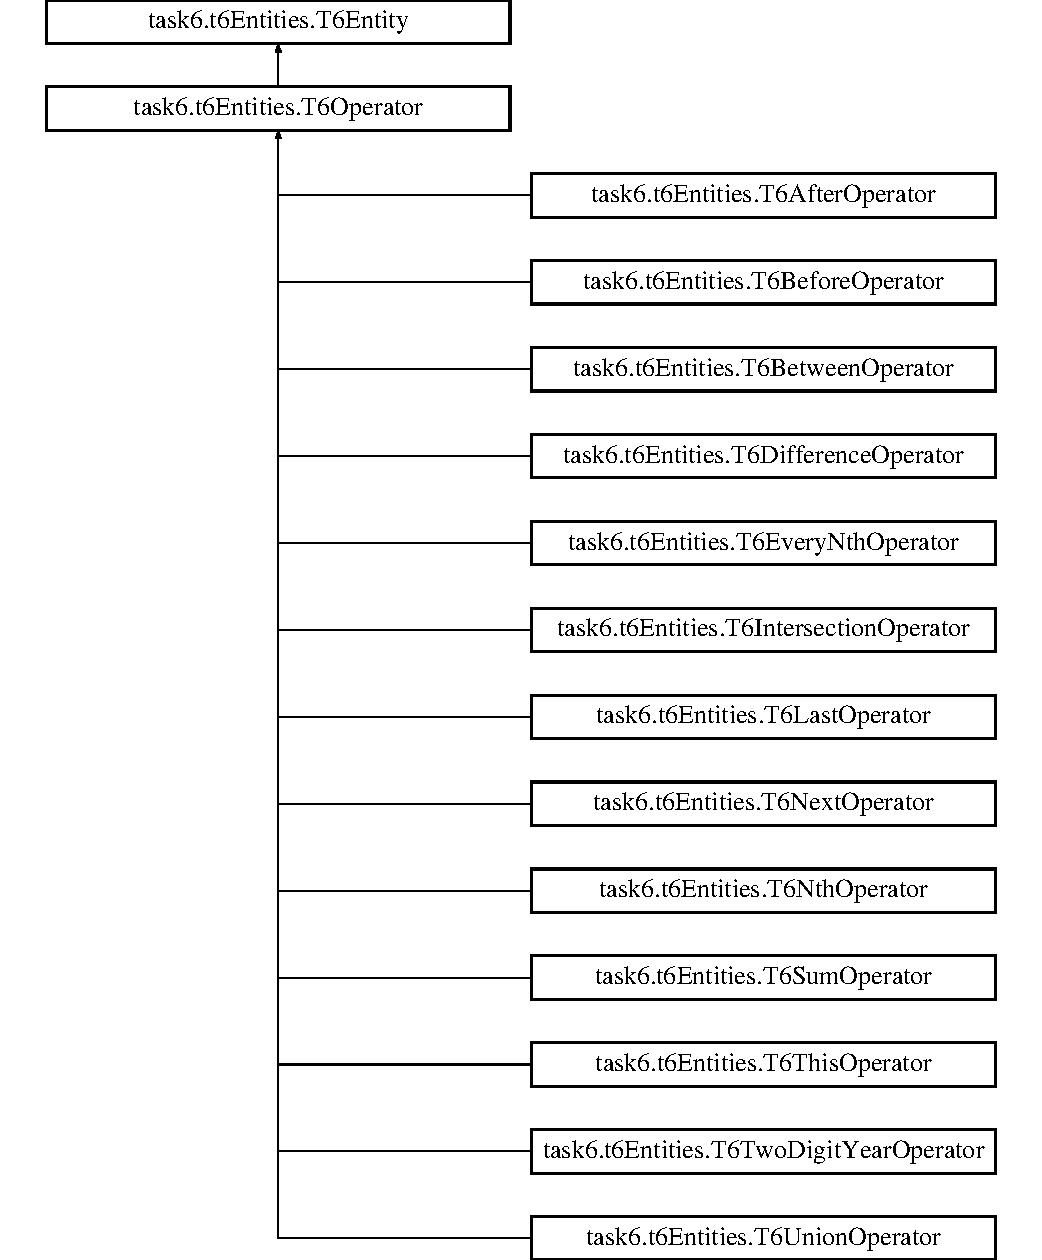
\includegraphics[height=12.000000cm]{classtask6_1_1t6Entities_1_1T6Operator}
\end{center}
\end{figure}
\subsection*{Public Member Functions}
\begin{DoxyCompactItemize}
\item 
def \hyperlink{classtask6_1_1t6Entities_1_1T6Operator_a2439f51a00c049e0e5e77472e2115b63}{\+\_\+\+\_\+init\+\_\+\+\_\+} (self, \hyperlink{classtask6_1_1t6Entities_1_1T6Entity_afeeced8134bb3ebe0cfecc64d0ab46a4}{id}, \hyperlink{classtask6_1_1t6Entities_1_1T6Entity_a52779e9af8864dc98e8b02fc5b9b041a}{start\+\_\+span}, \hyperlink{classtask6_1_1t6Entities_1_1T6Entity_aeb402200b156cd9562c5111dfe777b98}{end\+\_\+span}, operator\+\_\+type)
\end{DoxyCompactItemize}
\subsection*{Additional Inherited Members}


\subsection{Detailed Description}


Definition at line 167 of file t6\+Entities.\+py.



\subsection{Constructor \& Destructor Documentation}
\mbox{\Hypertarget{classtask6_1_1t6Entities_1_1T6Operator_a2439f51a00c049e0e5e77472e2115b63}\label{classtask6_1_1t6Entities_1_1T6Operator_a2439f51a00c049e0e5e77472e2115b63}} 
\index{task6\+::t6\+Entities\+::\+T6\+Operator@{task6\+::t6\+Entities\+::\+T6\+Operator}!\+\_\+\+\_\+init\+\_\+\+\_\+@{\+\_\+\+\_\+init\+\_\+\+\_\+}}
\index{\+\_\+\+\_\+init\+\_\+\+\_\+@{\+\_\+\+\_\+init\+\_\+\+\_\+}!task6\+::t6\+Entities\+::\+T6\+Operator@{task6\+::t6\+Entities\+::\+T6\+Operator}}
\subsubsection{\texorpdfstring{\+\_\+\+\_\+init\+\_\+\+\_\+()}{\_\_init\_\_()}}
{\footnotesize\ttfamily def task6.\+t6\+Entities.\+T6\+Operator.\+\_\+\+\_\+init\+\_\+\+\_\+ (\begin{DoxyParamCaption}\item[{}]{self,  }\item[{}]{id,  }\item[{}]{start\+\_\+span,  }\item[{}]{end\+\_\+span,  }\item[{}]{operator\+\_\+type }\end{DoxyParamCaption})}



Definition at line 168 of file t6\+Entities.\+py.



The documentation for this class was generated from the following file\+:\begin{DoxyCompactItemize}
\item 
task6/\hyperlink{t6Entities_8py}{t6\+Entities.\+py}\end{DoxyCompactItemize}

\hypertarget{classtask6_1_1t6Entities_1_1T6PartOfDayEntity}{}\section{task6.\+t6\+Entities.\+T6\+Part\+Of\+Day\+Entity Class Reference}
\label{classtask6_1_1t6Entities_1_1T6PartOfDayEntity}\index{task6.\+t6\+Entities.\+T6\+Part\+Of\+Day\+Entity@{task6.\+t6\+Entities.\+T6\+Part\+Of\+Day\+Entity}}
Inheritance diagram for task6.\+t6\+Entities.\+T6\+Part\+Of\+Day\+Entity\+:\begin{figure}[H]
\begin{center}
\leavevmode
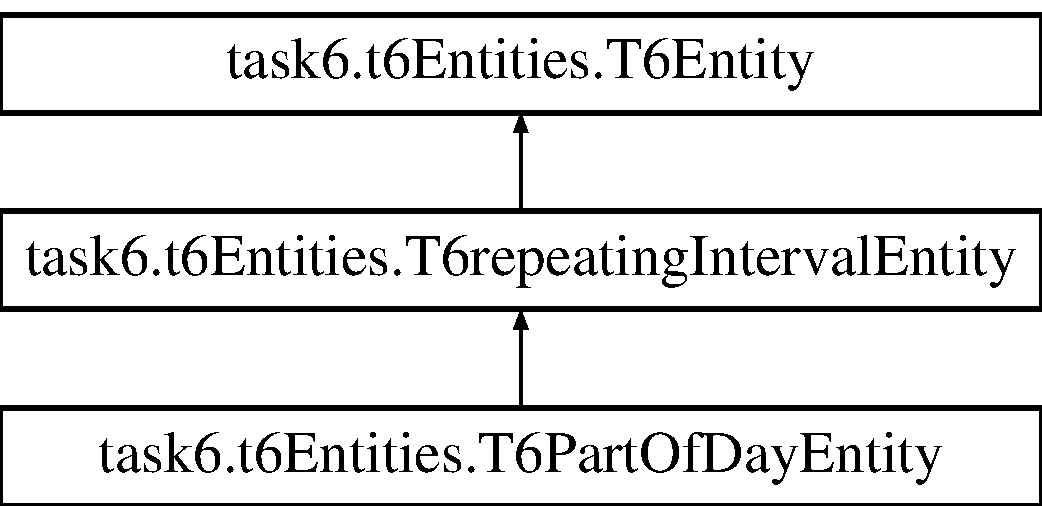
\includegraphics[height=3.000000cm]{classtask6_1_1t6Entities_1_1T6PartOfDayEntity}
\end{center}
\end{figure}
\subsection*{Public Member Functions}
\begin{DoxyCompactItemize}
\item 
def \hyperlink{classtask6_1_1t6Entities_1_1T6PartOfDayEntity_a0ead37bbbdc71d0de29a6433728dd8ad}{\+\_\+\+\_\+init\+\_\+\+\_\+} (self, \hyperlink{classtask6_1_1t6Entities_1_1T6Entity_afeeced8134bb3ebe0cfecc64d0ab46a4}{id}, \hyperlink{classtask6_1_1t6Entities_1_1T6Entity_a52779e9af8864dc98e8b02fc5b9b041a}{start\+\_\+span}, \hyperlink{classtask6_1_1t6Entities_1_1T6Entity_aeb402200b156cd9562c5111dfe777b98}{end\+\_\+span}, \hyperlink{classtask6_1_1t6Entities_1_1T6PartOfDayEntity_a402e24a798ab8edff4fde1691dbc0804}{part\+\_\+of\+\_\+day\+\_\+type}, \hyperlink{classtask6_1_1t6Entities_1_1T6PartOfDayEntity_a79992bc771c372834736b93aedfa428f}{number}, \hyperlink{classtask6_1_1t6Entities_1_1T6PartOfDayEntity_a83c5083b560f5295d713af2fc5013748}{modifier})
\end{DoxyCompactItemize}
\subsection*{Public Attributes}
\begin{DoxyCompactItemize}
\item 
\hyperlink{classtask6_1_1t6Entities_1_1T6PartOfDayEntity_a402e24a798ab8edff4fde1691dbc0804}{part\+\_\+of\+\_\+day\+\_\+type}
\item 
\hyperlink{classtask6_1_1t6Entities_1_1T6PartOfDayEntity_a79992bc771c372834736b93aedfa428f}{number}
\item 
\hyperlink{classtask6_1_1t6Entities_1_1T6PartOfDayEntity_a83c5083b560f5295d713af2fc5013748}{modifier}
\end{DoxyCompactItemize}


\subsection{Detailed Description}


Definition at line 149 of file t6\+Entities.\+py.



\subsection{Constructor \& Destructor Documentation}
\mbox{\Hypertarget{classtask6_1_1t6Entities_1_1T6PartOfDayEntity_a0ead37bbbdc71d0de29a6433728dd8ad}\label{classtask6_1_1t6Entities_1_1T6PartOfDayEntity_a0ead37bbbdc71d0de29a6433728dd8ad}} 
\index{task6\+::t6\+Entities\+::\+T6\+Part\+Of\+Day\+Entity@{task6\+::t6\+Entities\+::\+T6\+Part\+Of\+Day\+Entity}!\+\_\+\+\_\+init\+\_\+\+\_\+@{\+\_\+\+\_\+init\+\_\+\+\_\+}}
\index{\+\_\+\+\_\+init\+\_\+\+\_\+@{\+\_\+\+\_\+init\+\_\+\+\_\+}!task6\+::t6\+Entities\+::\+T6\+Part\+Of\+Day\+Entity@{task6\+::t6\+Entities\+::\+T6\+Part\+Of\+Day\+Entity}}
\subsubsection{\texorpdfstring{\+\_\+\+\_\+init\+\_\+\+\_\+()}{\_\_init\_\_()}}
{\footnotesize\ttfamily def task6.\+t6\+Entities.\+T6\+Part\+Of\+Day\+Entity.\+\_\+\+\_\+init\+\_\+\+\_\+ (\begin{DoxyParamCaption}\item[{}]{self,  }\item[{}]{id,  }\item[{}]{start\+\_\+span,  }\item[{}]{end\+\_\+span,  }\item[{}]{part\+\_\+of\+\_\+day\+\_\+type,  }\item[{}]{number,  }\item[{}]{modifier }\end{DoxyParamCaption})}



Definition at line 150 of file t6\+Entities.\+py.



\subsection{Member Data Documentation}
\mbox{\Hypertarget{classtask6_1_1t6Entities_1_1T6PartOfDayEntity_a83c5083b560f5295d713af2fc5013748}\label{classtask6_1_1t6Entities_1_1T6PartOfDayEntity_a83c5083b560f5295d713af2fc5013748}} 
\index{task6\+::t6\+Entities\+::\+T6\+Part\+Of\+Day\+Entity@{task6\+::t6\+Entities\+::\+T6\+Part\+Of\+Day\+Entity}!modifier@{modifier}}
\index{modifier@{modifier}!task6\+::t6\+Entities\+::\+T6\+Part\+Of\+Day\+Entity@{task6\+::t6\+Entities\+::\+T6\+Part\+Of\+Day\+Entity}}
\subsubsection{\texorpdfstring{modifier}{modifier}}
{\footnotesize\ttfamily task6.\+t6\+Entities.\+T6\+Part\+Of\+Day\+Entity.\+modifier}



Definition at line 154 of file t6\+Entities.\+py.

\mbox{\Hypertarget{classtask6_1_1t6Entities_1_1T6PartOfDayEntity_a79992bc771c372834736b93aedfa428f}\label{classtask6_1_1t6Entities_1_1T6PartOfDayEntity_a79992bc771c372834736b93aedfa428f}} 
\index{task6\+::t6\+Entities\+::\+T6\+Part\+Of\+Day\+Entity@{task6\+::t6\+Entities\+::\+T6\+Part\+Of\+Day\+Entity}!number@{number}}
\index{number@{number}!task6\+::t6\+Entities\+::\+T6\+Part\+Of\+Day\+Entity@{task6\+::t6\+Entities\+::\+T6\+Part\+Of\+Day\+Entity}}
\subsubsection{\texorpdfstring{number}{number}}
{\footnotesize\ttfamily task6.\+t6\+Entities.\+T6\+Part\+Of\+Day\+Entity.\+number}



Definition at line 153 of file t6\+Entities.\+py.

\mbox{\Hypertarget{classtask6_1_1t6Entities_1_1T6PartOfDayEntity_a402e24a798ab8edff4fde1691dbc0804}\label{classtask6_1_1t6Entities_1_1T6PartOfDayEntity_a402e24a798ab8edff4fde1691dbc0804}} 
\index{task6\+::t6\+Entities\+::\+T6\+Part\+Of\+Day\+Entity@{task6\+::t6\+Entities\+::\+T6\+Part\+Of\+Day\+Entity}!part\+\_\+of\+\_\+day\+\_\+type@{part\+\_\+of\+\_\+day\+\_\+type}}
\index{part\+\_\+of\+\_\+day\+\_\+type@{part\+\_\+of\+\_\+day\+\_\+type}!task6\+::t6\+Entities\+::\+T6\+Part\+Of\+Day\+Entity@{task6\+::t6\+Entities\+::\+T6\+Part\+Of\+Day\+Entity}}
\subsubsection{\texorpdfstring{part\+\_\+of\+\_\+day\+\_\+type}{part\_of\_day\_type}}
{\footnotesize\ttfamily task6.\+t6\+Entities.\+T6\+Part\+Of\+Day\+Entity.\+part\+\_\+of\+\_\+day\+\_\+type}



Definition at line 152 of file t6\+Entities.\+py.



The documentation for this class was generated from the following file\+:\begin{DoxyCompactItemize}
\item 
task6/\hyperlink{t6Entities_8py}{t6\+Entities.\+py}\end{DoxyCompactItemize}

\hypertarget{classtask6_1_1t6Entities_1_1T6PeriodEntity}{}\section{task6.\+t6\+Entities.\+T6\+Period\+Entity Class Reference}
\label{classtask6_1_1t6Entities_1_1T6PeriodEntity}\index{task6.\+t6\+Entities.\+T6\+Period\+Entity@{task6.\+t6\+Entities.\+T6\+Period\+Entity}}
Inheritance diagram for task6.\+t6\+Entities.\+T6\+Period\+Entity\+:\begin{figure}[H]
\begin{center}
\leavevmode
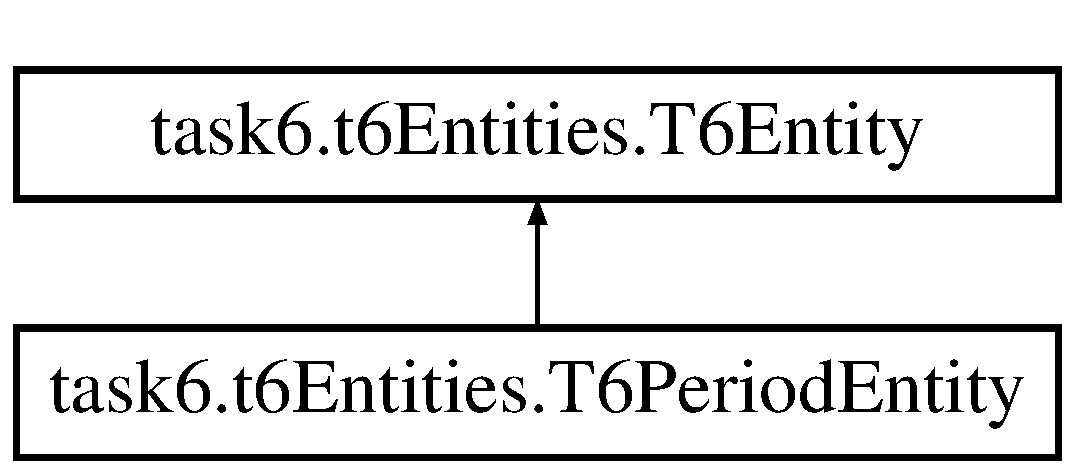
\includegraphics[height=2.000000cm]{classtask6_1_1t6Entities_1_1T6PeriodEntity}
\end{center}
\end{figure}
\subsection*{Public Member Functions}
\begin{DoxyCompactItemize}
\item 
def \hyperlink{classtask6_1_1t6Entities_1_1T6PeriodEntity_a2641256b4427ad07e9041d9f389a551d}{\+\_\+\+\_\+init\+\_\+\+\_\+} (self, \hyperlink{classtask6_1_1t6Entities_1_1T6Entity_afeeced8134bb3ebe0cfecc64d0ab46a4}{id}, \hyperlink{classtask6_1_1t6Entities_1_1T6Entity_a52779e9af8864dc98e8b02fc5b9b041a}{start\+\_\+span}, \hyperlink{classtask6_1_1t6Entities_1_1T6Entity_aeb402200b156cd9562c5111dfe777b98}{end\+\_\+span}, \hyperlink{classtask6_1_1t6Entities_1_1T6PeriodEntity_aa40d8fd07038f68f3f918a09fb0d1beb}{period\+\_\+type}=None, \hyperlink{classtask6_1_1t6Entities_1_1T6PeriodEntity_ae1a98d39cfb27a8dd99f3b54f35b4b14}{number}=None, \hyperlink{classtask6_1_1t6Entities_1_1T6PeriodEntity_a6ac8572830e19053387210cda80a8970}{modifier}=None)
\end{DoxyCompactItemize}
\subsection*{Public Attributes}
\begin{DoxyCompactItemize}
\item 
\hyperlink{classtask6_1_1t6Entities_1_1T6PeriodEntity_aa40d8fd07038f68f3f918a09fb0d1beb}{period\+\_\+type}
\item 
\hyperlink{classtask6_1_1t6Entities_1_1T6PeriodEntity_ae1a98d39cfb27a8dd99f3b54f35b4b14}{number}
\item 
\hyperlink{classtask6_1_1t6Entities_1_1T6PeriodEntity_a6ac8572830e19053387210cda80a8970}{modifier}
\end{DoxyCompactItemize}


\subsection{Detailed Description}


Definition at line 75 of file t6\+Entities.\+py.



\subsection{Constructor \& Destructor Documentation}
\mbox{\Hypertarget{classtask6_1_1t6Entities_1_1T6PeriodEntity_a2641256b4427ad07e9041d9f389a551d}\label{classtask6_1_1t6Entities_1_1T6PeriodEntity_a2641256b4427ad07e9041d9f389a551d}} 
\index{task6\+::t6\+Entities\+::\+T6\+Period\+Entity@{task6\+::t6\+Entities\+::\+T6\+Period\+Entity}!\+\_\+\+\_\+init\+\_\+\+\_\+@{\+\_\+\+\_\+init\+\_\+\+\_\+}}
\index{\+\_\+\+\_\+init\+\_\+\+\_\+@{\+\_\+\+\_\+init\+\_\+\+\_\+}!task6\+::t6\+Entities\+::\+T6\+Period\+Entity@{task6\+::t6\+Entities\+::\+T6\+Period\+Entity}}
\subsubsection{\texorpdfstring{\+\_\+\+\_\+init\+\_\+\+\_\+()}{\_\_init\_\_()}}
{\footnotesize\ttfamily def task6.\+t6\+Entities.\+T6\+Period\+Entity.\+\_\+\+\_\+init\+\_\+\+\_\+ (\begin{DoxyParamCaption}\item[{}]{self,  }\item[{}]{id,  }\item[{}]{start\+\_\+span,  }\item[{}]{end\+\_\+span,  }\item[{}]{period\+\_\+type = {\ttfamily None},  }\item[{}]{number = {\ttfamily None},  }\item[{}]{modifier = {\ttfamily None} }\end{DoxyParamCaption})}



Definition at line 76 of file t6\+Entities.\+py.



\subsection{Member Data Documentation}
\mbox{\Hypertarget{classtask6_1_1t6Entities_1_1T6PeriodEntity_a6ac8572830e19053387210cda80a8970}\label{classtask6_1_1t6Entities_1_1T6PeriodEntity_a6ac8572830e19053387210cda80a8970}} 
\index{task6\+::t6\+Entities\+::\+T6\+Period\+Entity@{task6\+::t6\+Entities\+::\+T6\+Period\+Entity}!modifier@{modifier}}
\index{modifier@{modifier}!task6\+::t6\+Entities\+::\+T6\+Period\+Entity@{task6\+::t6\+Entities\+::\+T6\+Period\+Entity}}
\subsubsection{\texorpdfstring{modifier}{modifier}}
{\footnotesize\ttfamily task6.\+t6\+Entities.\+T6\+Period\+Entity.\+modifier}



Definition at line 80 of file t6\+Entities.\+py.

\mbox{\Hypertarget{classtask6_1_1t6Entities_1_1T6PeriodEntity_ae1a98d39cfb27a8dd99f3b54f35b4b14}\label{classtask6_1_1t6Entities_1_1T6PeriodEntity_ae1a98d39cfb27a8dd99f3b54f35b4b14}} 
\index{task6\+::t6\+Entities\+::\+T6\+Period\+Entity@{task6\+::t6\+Entities\+::\+T6\+Period\+Entity}!number@{number}}
\index{number@{number}!task6\+::t6\+Entities\+::\+T6\+Period\+Entity@{task6\+::t6\+Entities\+::\+T6\+Period\+Entity}}
\subsubsection{\texorpdfstring{number}{number}}
{\footnotesize\ttfamily task6.\+t6\+Entities.\+T6\+Period\+Entity.\+number}



Definition at line 79 of file t6\+Entities.\+py.

\mbox{\Hypertarget{classtask6_1_1t6Entities_1_1T6PeriodEntity_aa40d8fd07038f68f3f918a09fb0d1beb}\label{classtask6_1_1t6Entities_1_1T6PeriodEntity_aa40d8fd07038f68f3f918a09fb0d1beb}} 
\index{task6\+::t6\+Entities\+::\+T6\+Period\+Entity@{task6\+::t6\+Entities\+::\+T6\+Period\+Entity}!period\+\_\+type@{period\+\_\+type}}
\index{period\+\_\+type@{period\+\_\+type}!task6\+::t6\+Entities\+::\+T6\+Period\+Entity@{task6\+::t6\+Entities\+::\+T6\+Period\+Entity}}
\subsubsection{\texorpdfstring{period\+\_\+type}{period\_type}}
{\footnotesize\ttfamily task6.\+t6\+Entities.\+T6\+Period\+Entity.\+period\+\_\+type}



Definition at line 78 of file t6\+Entities.\+py.



The documentation for this class was generated from the following file\+:\begin{DoxyCompactItemize}
\item 
task6/\hyperlink{t6Entities_8py}{t6\+Entities.\+py}\end{DoxyCompactItemize}

\hypertarget{classtask6_1_1t6Entities_1_1T6repeatingIntervalEntity}{}\section{task6.\+t6\+Entities.\+T6repeating\+Interval\+Entity Class Reference}
\label{classtask6_1_1t6Entities_1_1T6repeatingIntervalEntity}\index{task6.\+t6\+Entities.\+T6repeating\+Interval\+Entity@{task6.\+t6\+Entities.\+T6repeating\+Interval\+Entity}}
Inheritance diagram for task6.\+t6\+Entities.\+T6repeating\+Interval\+Entity\+:\begin{figure}[H]
\begin{center}
\leavevmode
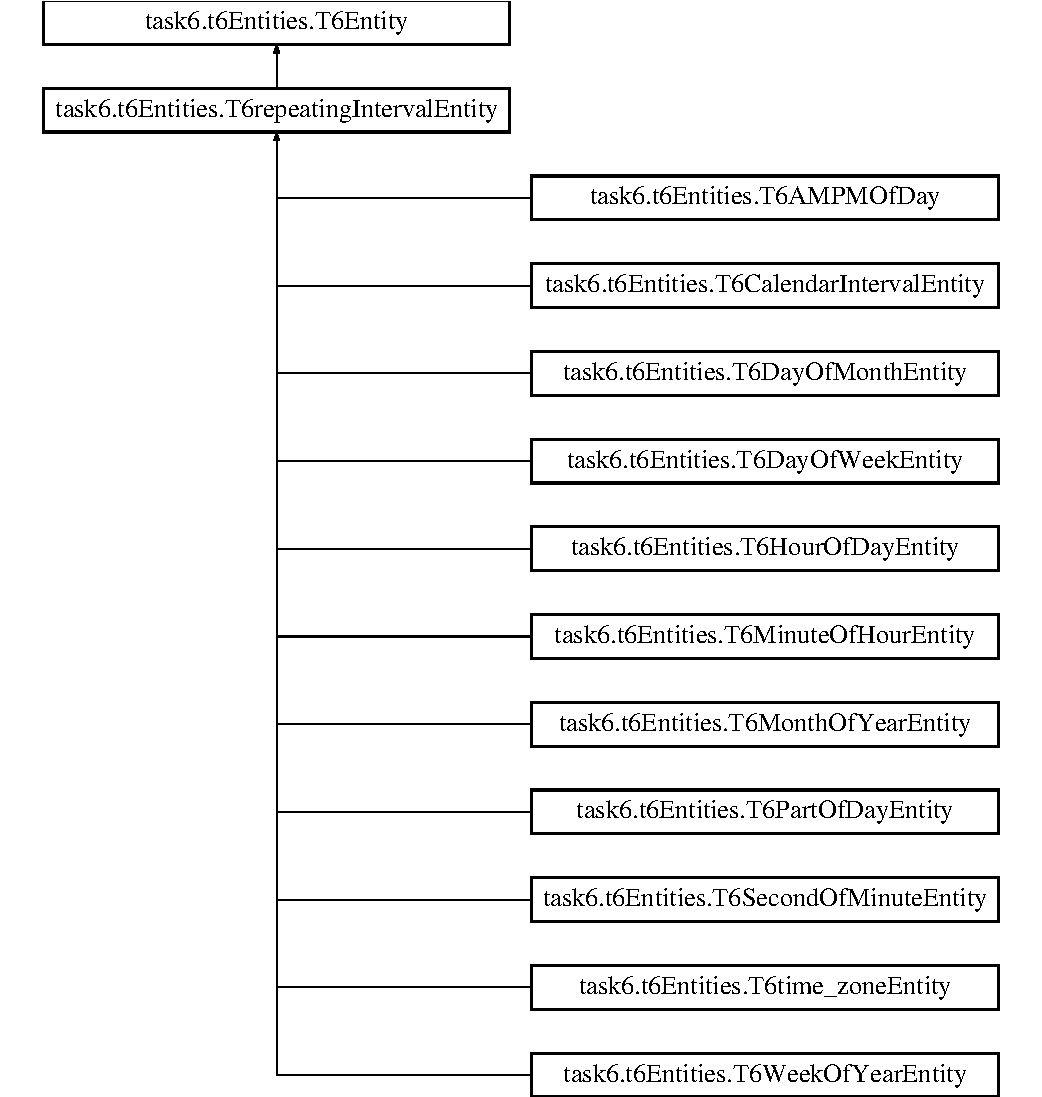
\includegraphics[height=12.000000cm]{classtask6_1_1t6Entities_1_1T6repeatingIntervalEntity}
\end{center}
\end{figure}
\subsection*{Public Member Functions}
\begin{DoxyCompactItemize}
\item 
def \hyperlink{classtask6_1_1t6Entities_1_1T6repeatingIntervalEntity_a26cfdfdfe5c9a22651112680c641c159}{\+\_\+\+\_\+init\+\_\+\+\_\+} (self, \hyperlink{classtask6_1_1t6Entities_1_1T6Entity_afeeced8134bb3ebe0cfecc64d0ab46a4}{id}, \hyperlink{classtask6_1_1t6Entities_1_1T6Entity_a52779e9af8864dc98e8b02fc5b9b041a}{start\+\_\+span}, \hyperlink{classtask6_1_1t6Entities_1_1T6Entity_aeb402200b156cd9562c5111dfe777b98}{end\+\_\+span}, \hyperlink{classtask6_1_1t6Entities_1_1T6Entity_ae4299399be3ecbd68dbb9ae988bff5a8}{type})
\end{DoxyCompactItemize}
\subsection*{Additional Inherited Members}


\subsection{Detailed Description}


Definition at line 82 of file t6\+Entities.\+py.



\subsection{Constructor \& Destructor Documentation}
\mbox{\Hypertarget{classtask6_1_1t6Entities_1_1T6repeatingIntervalEntity_a26cfdfdfe5c9a22651112680c641c159}\label{classtask6_1_1t6Entities_1_1T6repeatingIntervalEntity_a26cfdfdfe5c9a22651112680c641c159}} 
\index{task6\+::t6\+Entities\+::\+T6repeating\+Interval\+Entity@{task6\+::t6\+Entities\+::\+T6repeating\+Interval\+Entity}!\+\_\+\+\_\+init\+\_\+\+\_\+@{\+\_\+\+\_\+init\+\_\+\+\_\+}}
\index{\+\_\+\+\_\+init\+\_\+\+\_\+@{\+\_\+\+\_\+init\+\_\+\+\_\+}!task6\+::t6\+Entities\+::\+T6repeating\+Interval\+Entity@{task6\+::t6\+Entities\+::\+T6repeating\+Interval\+Entity}}
\subsubsection{\texorpdfstring{\+\_\+\+\_\+init\+\_\+\+\_\+()}{\_\_init\_\_()}}
{\footnotesize\ttfamily def task6.\+t6\+Entities.\+T6repeating\+Interval\+Entity.\+\_\+\+\_\+init\+\_\+\+\_\+ (\begin{DoxyParamCaption}\item[{}]{self,  }\item[{}]{id,  }\item[{}]{start\+\_\+span,  }\item[{}]{end\+\_\+span,  }\item[{}]{type }\end{DoxyParamCaption})}



Definition at line 83 of file t6\+Entities.\+py.



The documentation for this class was generated from the following file\+:\begin{DoxyCompactItemize}
\item 
task6/\hyperlink{t6Entities_8py}{t6\+Entities.\+py}\end{DoxyCompactItemize}

\hypertarget{classtask6_1_1t6Entities_1_1T6SecondOfMinuteEntity}{}\section{task6.\+t6\+Entities.\+T6\+Second\+Of\+Minute\+Entity Class Reference}
\label{classtask6_1_1t6Entities_1_1T6SecondOfMinuteEntity}\index{task6.\+t6\+Entities.\+T6\+Second\+Of\+Minute\+Entity@{task6.\+t6\+Entities.\+T6\+Second\+Of\+Minute\+Entity}}
Inheritance diagram for task6.\+t6\+Entities.\+T6\+Second\+Of\+Minute\+Entity\+:\begin{figure}[H]
\begin{center}
\leavevmode
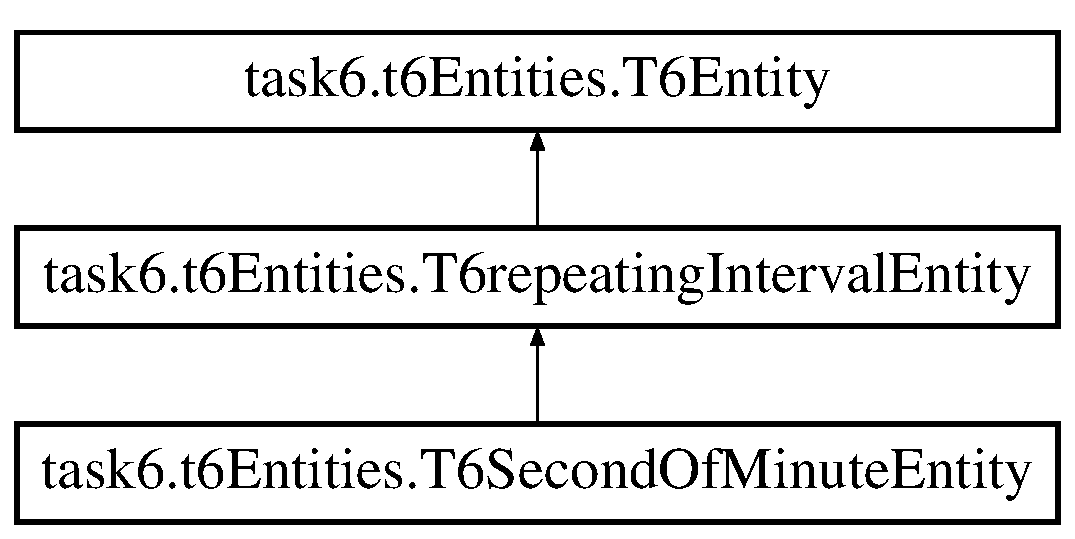
\includegraphics[height=3.000000cm]{classtask6_1_1t6Entities_1_1T6SecondOfMinuteEntity}
\end{center}
\end{figure}
\subsection*{Public Member Functions}
\begin{DoxyCompactItemize}
\item 
def \hyperlink{classtask6_1_1t6Entities_1_1T6SecondOfMinuteEntity_a3523b619b18a5e697d9cb943d16cf482}{\+\_\+\+\_\+init\+\_\+\+\_\+} (self, \hyperlink{classtask6_1_1t6Entities_1_1T6Entity_afeeced8134bb3ebe0cfecc64d0ab46a4}{id}, \hyperlink{classtask6_1_1t6Entities_1_1T6Entity_a52779e9af8864dc98e8b02fc5b9b041a}{start\+\_\+span}, \hyperlink{classtask6_1_1t6Entities_1_1T6Entity_aeb402200b156cd9562c5111dfe777b98}{end\+\_\+span}, \hyperlink{classtask6_1_1t6Entities_1_1T6SecondOfMinuteEntity_a953e8f418d52f6d7086b15bcc9c09b45}{value}, \hyperlink{classtask6_1_1t6Entities_1_1T6SecondOfMinuteEntity_a9a7d83f3f2e73db26b4471180b862fa0}{number}, \hyperlink{classtask6_1_1t6Entities_1_1T6SecondOfMinuteEntity_a611814e0a295d6a80e296f1ea02e10c4}{modifier})
\end{DoxyCompactItemize}
\subsection*{Public Attributes}
\begin{DoxyCompactItemize}
\item 
\hyperlink{classtask6_1_1t6Entities_1_1T6SecondOfMinuteEntity_a953e8f418d52f6d7086b15bcc9c09b45}{value}
\item 
\hyperlink{classtask6_1_1t6Entities_1_1T6SecondOfMinuteEntity_a9a7d83f3f2e73db26b4471180b862fa0}{number}
\item 
\hyperlink{classtask6_1_1t6Entities_1_1T6SecondOfMinuteEntity_a611814e0a295d6a80e296f1ea02e10c4}{modifier}
\end{DoxyCompactItemize}


\subsection{Detailed Description}


Definition at line 135 of file t6\+Entities.\+py.



\subsection{Constructor \& Destructor Documentation}
\mbox{\Hypertarget{classtask6_1_1t6Entities_1_1T6SecondOfMinuteEntity_a3523b619b18a5e697d9cb943d16cf482}\label{classtask6_1_1t6Entities_1_1T6SecondOfMinuteEntity_a3523b619b18a5e697d9cb943d16cf482}} 
\index{task6\+::t6\+Entities\+::\+T6\+Second\+Of\+Minute\+Entity@{task6\+::t6\+Entities\+::\+T6\+Second\+Of\+Minute\+Entity}!\+\_\+\+\_\+init\+\_\+\+\_\+@{\+\_\+\+\_\+init\+\_\+\+\_\+}}
\index{\+\_\+\+\_\+init\+\_\+\+\_\+@{\+\_\+\+\_\+init\+\_\+\+\_\+}!task6\+::t6\+Entities\+::\+T6\+Second\+Of\+Minute\+Entity@{task6\+::t6\+Entities\+::\+T6\+Second\+Of\+Minute\+Entity}}
\subsubsection{\texorpdfstring{\+\_\+\+\_\+init\+\_\+\+\_\+()}{\_\_init\_\_()}}
{\footnotesize\ttfamily def task6.\+t6\+Entities.\+T6\+Second\+Of\+Minute\+Entity.\+\_\+\+\_\+init\+\_\+\+\_\+ (\begin{DoxyParamCaption}\item[{}]{self,  }\item[{}]{id,  }\item[{}]{start\+\_\+span,  }\item[{}]{end\+\_\+span,  }\item[{}]{value,  }\item[{}]{number,  }\item[{}]{modifier }\end{DoxyParamCaption})}



Definition at line 136 of file t6\+Entities.\+py.



\subsection{Member Data Documentation}
\mbox{\Hypertarget{classtask6_1_1t6Entities_1_1T6SecondOfMinuteEntity_a611814e0a295d6a80e296f1ea02e10c4}\label{classtask6_1_1t6Entities_1_1T6SecondOfMinuteEntity_a611814e0a295d6a80e296f1ea02e10c4}} 
\index{task6\+::t6\+Entities\+::\+T6\+Second\+Of\+Minute\+Entity@{task6\+::t6\+Entities\+::\+T6\+Second\+Of\+Minute\+Entity}!modifier@{modifier}}
\index{modifier@{modifier}!task6\+::t6\+Entities\+::\+T6\+Second\+Of\+Minute\+Entity@{task6\+::t6\+Entities\+::\+T6\+Second\+Of\+Minute\+Entity}}
\subsubsection{\texorpdfstring{modifier}{modifier}}
{\footnotesize\ttfamily task6.\+t6\+Entities.\+T6\+Second\+Of\+Minute\+Entity.\+modifier}



Definition at line 140 of file t6\+Entities.\+py.

\mbox{\Hypertarget{classtask6_1_1t6Entities_1_1T6SecondOfMinuteEntity_a9a7d83f3f2e73db26b4471180b862fa0}\label{classtask6_1_1t6Entities_1_1T6SecondOfMinuteEntity_a9a7d83f3f2e73db26b4471180b862fa0}} 
\index{task6\+::t6\+Entities\+::\+T6\+Second\+Of\+Minute\+Entity@{task6\+::t6\+Entities\+::\+T6\+Second\+Of\+Minute\+Entity}!number@{number}}
\index{number@{number}!task6\+::t6\+Entities\+::\+T6\+Second\+Of\+Minute\+Entity@{task6\+::t6\+Entities\+::\+T6\+Second\+Of\+Minute\+Entity}}
\subsubsection{\texorpdfstring{number}{number}}
{\footnotesize\ttfamily task6.\+t6\+Entities.\+T6\+Second\+Of\+Minute\+Entity.\+number}



Definition at line 139 of file t6\+Entities.\+py.

\mbox{\Hypertarget{classtask6_1_1t6Entities_1_1T6SecondOfMinuteEntity_a953e8f418d52f6d7086b15bcc9c09b45}\label{classtask6_1_1t6Entities_1_1T6SecondOfMinuteEntity_a953e8f418d52f6d7086b15bcc9c09b45}} 
\index{task6\+::t6\+Entities\+::\+T6\+Second\+Of\+Minute\+Entity@{task6\+::t6\+Entities\+::\+T6\+Second\+Of\+Minute\+Entity}!value@{value}}
\index{value@{value}!task6\+::t6\+Entities\+::\+T6\+Second\+Of\+Minute\+Entity@{task6\+::t6\+Entities\+::\+T6\+Second\+Of\+Minute\+Entity}}
\subsubsection{\texorpdfstring{value}{value}}
{\footnotesize\ttfamily task6.\+t6\+Entities.\+T6\+Second\+Of\+Minute\+Entity.\+value}



Definition at line 138 of file t6\+Entities.\+py.



The documentation for this class was generated from the following file\+:\begin{DoxyCompactItemize}
\item 
task6/\hyperlink{t6Entities_8py}{t6\+Entities.\+py}\end{DoxyCompactItemize}

\hypertarget{classtask6_1_1t6Entities_1_1T6SumOperator}{}\section{task6.\+t6\+Entities.\+T6\+Sum\+Operator Class Reference}
\label{classtask6_1_1t6Entities_1_1T6SumOperator}\index{task6.\+t6\+Entities.\+T6\+Sum\+Operator@{task6.\+t6\+Entities.\+T6\+Sum\+Operator}}
Inheritance diagram for task6.\+t6\+Entities.\+T6\+Sum\+Operator\+:\begin{figure}[H]
\begin{center}
\leavevmode
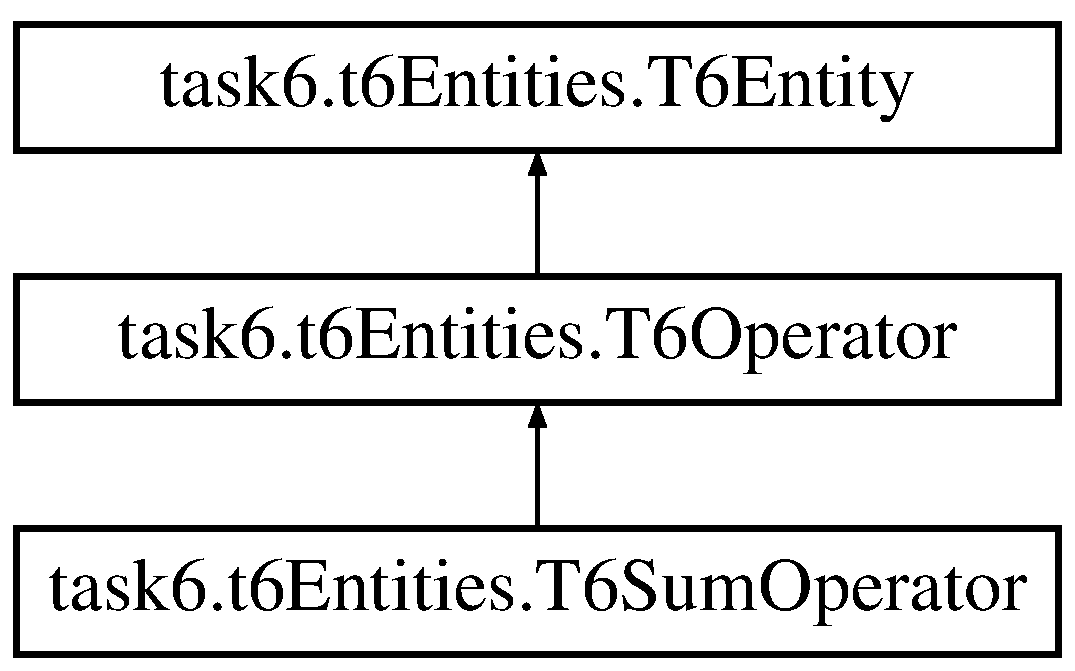
\includegraphics[height=3.000000cm]{classtask6_1_1t6Entities_1_1T6SumOperator}
\end{center}
\end{figure}
\subsection*{Public Member Functions}
\begin{DoxyCompactItemize}
\item 
def \hyperlink{classtask6_1_1t6Entities_1_1T6SumOperator_aa25af851f88d2574f2012834b7c86e81}{\+\_\+\+\_\+init\+\_\+\+\_\+} (self, \hyperlink{classtask6_1_1t6Entities_1_1T6Entity_afeeced8134bb3ebe0cfecc64d0ab46a4}{id}, \hyperlink{classtask6_1_1t6Entities_1_1T6Entity_a52779e9af8864dc98e8b02fc5b9b041a}{start\+\_\+span}, \hyperlink{classtask6_1_1t6Entities_1_1T6Entity_aeb402200b156cd9562c5111dfe777b98}{end\+\_\+span})
\end{DoxyCompactItemize}
\subsection*{Additional Inherited Members}


\subsection{Detailed Description}


Definition at line 172 of file t6\+Entities.\+py.



\subsection{Constructor \& Destructor Documentation}
\mbox{\Hypertarget{classtask6_1_1t6Entities_1_1T6SumOperator_aa25af851f88d2574f2012834b7c86e81}\label{classtask6_1_1t6Entities_1_1T6SumOperator_aa25af851f88d2574f2012834b7c86e81}} 
\index{task6\+::t6\+Entities\+::\+T6\+Sum\+Operator@{task6\+::t6\+Entities\+::\+T6\+Sum\+Operator}!\+\_\+\+\_\+init\+\_\+\+\_\+@{\+\_\+\+\_\+init\+\_\+\+\_\+}}
\index{\+\_\+\+\_\+init\+\_\+\+\_\+@{\+\_\+\+\_\+init\+\_\+\+\_\+}!task6\+::t6\+Entities\+::\+T6\+Sum\+Operator@{task6\+::t6\+Entities\+::\+T6\+Sum\+Operator}}
\subsubsection{\texorpdfstring{\+\_\+\+\_\+init\+\_\+\+\_\+()}{\_\_init\_\_()}}
{\footnotesize\ttfamily def task6.\+t6\+Entities.\+T6\+Sum\+Operator.\+\_\+\+\_\+init\+\_\+\+\_\+ (\begin{DoxyParamCaption}\item[{}]{self,  }\item[{}]{id,  }\item[{}]{start\+\_\+span,  }\item[{}]{end\+\_\+span }\end{DoxyParamCaption})}



Definition at line 173 of file t6\+Entities.\+py.



The documentation for this class was generated from the following file\+:\begin{DoxyCompactItemize}
\item 
task6/\hyperlink{t6Entities_8py}{t6\+Entities.\+py}\end{DoxyCompactItemize}

\hypertarget{classtask6_1_1t6Entities_1_1T6ThisOperator}{}\section{task6.\+t6\+Entities.\+T6\+This\+Operator Class Reference}
\label{classtask6_1_1t6Entities_1_1T6ThisOperator}\index{task6.\+t6\+Entities.\+T6\+This\+Operator@{task6.\+t6\+Entities.\+T6\+This\+Operator}}
Inheritance diagram for task6.\+t6\+Entities.\+T6\+This\+Operator\+:\begin{figure}[H]
\begin{center}
\leavevmode
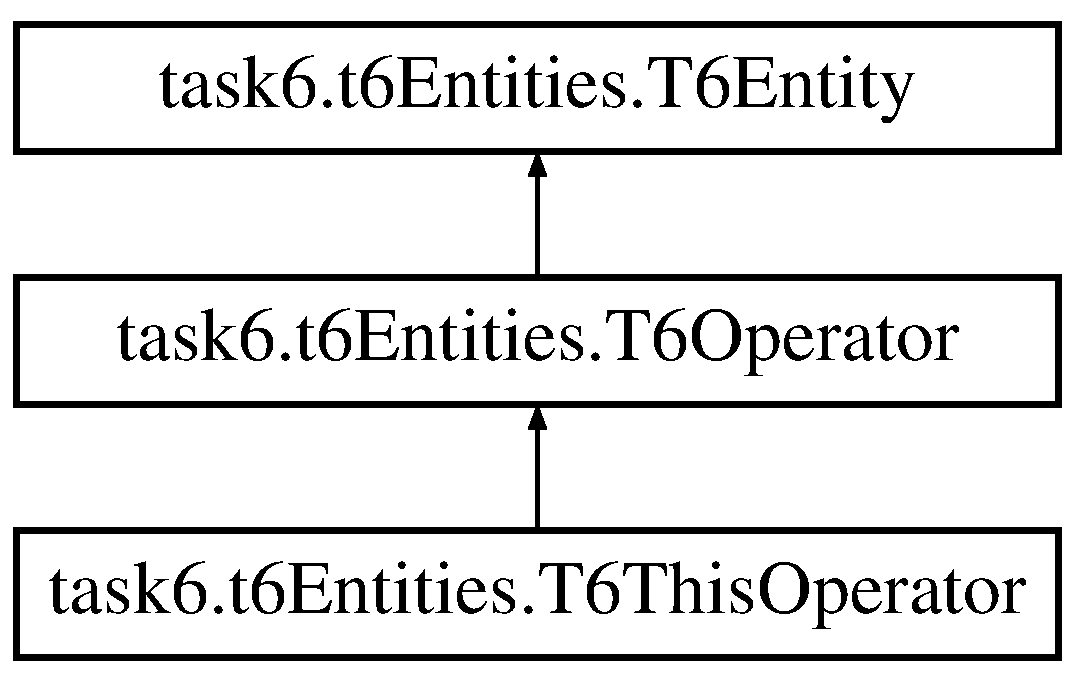
\includegraphics[height=3.000000cm]{classtask6_1_1t6Entities_1_1T6ThisOperator}
\end{center}
\end{figure}
\subsection*{Public Member Functions}
\begin{DoxyCompactItemize}
\item 
def \hyperlink{classtask6_1_1t6Entities_1_1T6ThisOperator_a3ff7e85bf38c12b6285d9af727c7290f}{\+\_\+\+\_\+init\+\_\+\+\_\+} (self, \hyperlink{classtask6_1_1t6Entities_1_1T6Entity_afeeced8134bb3ebe0cfecc64d0ab46a4}{id}, \hyperlink{classtask6_1_1t6Entities_1_1T6Entity_a52779e9af8864dc98e8b02fc5b9b041a}{start\+\_\+span}, \hyperlink{classtask6_1_1t6Entities_1_1T6Entity_aeb402200b156cd9562c5111dfe777b98}{end\+\_\+span}, \hyperlink{classtask6_1_1t6Entities_1_1T6ThisOperator_a4237e7eb65230f550e70c7979aa76286}{interval\+\_\+type}, \hyperlink{classtask6_1_1t6Entities_1_1T6ThisOperator_adadb6bba14cc5adcdaad1c585907061d}{interval}, \hyperlink{classtask6_1_1t6Entities_1_1T6ThisOperator_ac35cef8f01d47ee15a85b1d284ab5d41}{period}, \hyperlink{classtask6_1_1t6Entities_1_1T6ThisOperator_a1e995a6c80ad81b118c76bbc200969ab}{repeating\+\_\+interval})
\end{DoxyCompactItemize}
\subsection*{Public Attributes}
\begin{DoxyCompactItemize}
\item 
\hyperlink{classtask6_1_1t6Entities_1_1T6ThisOperator_a4237e7eb65230f550e70c7979aa76286}{interval\+\_\+type}
\item 
\hyperlink{classtask6_1_1t6Entities_1_1T6ThisOperator_adadb6bba14cc5adcdaad1c585907061d}{interval}
\item 
\hyperlink{classtask6_1_1t6Entities_1_1T6ThisOperator_ac35cef8f01d47ee15a85b1d284ab5d41}{period}
\item 
\hyperlink{classtask6_1_1t6Entities_1_1T6ThisOperator_a1e995a6c80ad81b118c76bbc200969ab}{repeating\+\_\+interval}
\end{DoxyCompactItemize}


\subsection{Detailed Description}


Definition at line 218 of file t6\+Entities.\+py.



\subsection{Constructor \& Destructor Documentation}
\mbox{\Hypertarget{classtask6_1_1t6Entities_1_1T6ThisOperator_a3ff7e85bf38c12b6285d9af727c7290f}\label{classtask6_1_1t6Entities_1_1T6ThisOperator_a3ff7e85bf38c12b6285d9af727c7290f}} 
\index{task6\+::t6\+Entities\+::\+T6\+This\+Operator@{task6\+::t6\+Entities\+::\+T6\+This\+Operator}!\+\_\+\+\_\+init\+\_\+\+\_\+@{\+\_\+\+\_\+init\+\_\+\+\_\+}}
\index{\+\_\+\+\_\+init\+\_\+\+\_\+@{\+\_\+\+\_\+init\+\_\+\+\_\+}!task6\+::t6\+Entities\+::\+T6\+This\+Operator@{task6\+::t6\+Entities\+::\+T6\+This\+Operator}}
\subsubsection{\texorpdfstring{\+\_\+\+\_\+init\+\_\+\+\_\+()}{\_\_init\_\_()}}
{\footnotesize\ttfamily def task6.\+t6\+Entities.\+T6\+This\+Operator.\+\_\+\+\_\+init\+\_\+\+\_\+ (\begin{DoxyParamCaption}\item[{}]{self,  }\item[{}]{id,  }\item[{}]{start\+\_\+span,  }\item[{}]{end\+\_\+span,  }\item[{}]{interval\+\_\+type,  }\item[{}]{interval,  }\item[{}]{period,  }\item[{}]{repeating\+\_\+interval }\end{DoxyParamCaption})}



Definition at line 219 of file t6\+Entities.\+py.



\subsection{Member Data Documentation}
\mbox{\Hypertarget{classtask6_1_1t6Entities_1_1T6ThisOperator_adadb6bba14cc5adcdaad1c585907061d}\label{classtask6_1_1t6Entities_1_1T6ThisOperator_adadb6bba14cc5adcdaad1c585907061d}} 
\index{task6\+::t6\+Entities\+::\+T6\+This\+Operator@{task6\+::t6\+Entities\+::\+T6\+This\+Operator}!interval@{interval}}
\index{interval@{interval}!task6\+::t6\+Entities\+::\+T6\+This\+Operator@{task6\+::t6\+Entities\+::\+T6\+This\+Operator}}
\subsubsection{\texorpdfstring{interval}{interval}}
{\footnotesize\ttfamily task6.\+t6\+Entities.\+T6\+This\+Operator.\+interval}



Definition at line 222 of file t6\+Entities.\+py.

\mbox{\Hypertarget{classtask6_1_1t6Entities_1_1T6ThisOperator_a4237e7eb65230f550e70c7979aa76286}\label{classtask6_1_1t6Entities_1_1T6ThisOperator_a4237e7eb65230f550e70c7979aa76286}} 
\index{task6\+::t6\+Entities\+::\+T6\+This\+Operator@{task6\+::t6\+Entities\+::\+T6\+This\+Operator}!interval\+\_\+type@{interval\+\_\+type}}
\index{interval\+\_\+type@{interval\+\_\+type}!task6\+::t6\+Entities\+::\+T6\+This\+Operator@{task6\+::t6\+Entities\+::\+T6\+This\+Operator}}
\subsubsection{\texorpdfstring{interval\+\_\+type}{interval\_type}}
{\footnotesize\ttfamily task6.\+t6\+Entities.\+T6\+This\+Operator.\+interval\+\_\+type}



Definition at line 221 of file t6\+Entities.\+py.

\mbox{\Hypertarget{classtask6_1_1t6Entities_1_1T6ThisOperator_ac35cef8f01d47ee15a85b1d284ab5d41}\label{classtask6_1_1t6Entities_1_1T6ThisOperator_ac35cef8f01d47ee15a85b1d284ab5d41}} 
\index{task6\+::t6\+Entities\+::\+T6\+This\+Operator@{task6\+::t6\+Entities\+::\+T6\+This\+Operator}!period@{period}}
\index{period@{period}!task6\+::t6\+Entities\+::\+T6\+This\+Operator@{task6\+::t6\+Entities\+::\+T6\+This\+Operator}}
\subsubsection{\texorpdfstring{period}{period}}
{\footnotesize\ttfamily task6.\+t6\+Entities.\+T6\+This\+Operator.\+period}



Definition at line 223 of file t6\+Entities.\+py.

\mbox{\Hypertarget{classtask6_1_1t6Entities_1_1T6ThisOperator_a1e995a6c80ad81b118c76bbc200969ab}\label{classtask6_1_1t6Entities_1_1T6ThisOperator_a1e995a6c80ad81b118c76bbc200969ab}} 
\index{task6\+::t6\+Entities\+::\+T6\+This\+Operator@{task6\+::t6\+Entities\+::\+T6\+This\+Operator}!repeating\+\_\+interval@{repeating\+\_\+interval}}
\index{repeating\+\_\+interval@{repeating\+\_\+interval}!task6\+::t6\+Entities\+::\+T6\+This\+Operator@{task6\+::t6\+Entities\+::\+T6\+This\+Operator}}
\subsubsection{\texorpdfstring{repeating\+\_\+interval}{repeating\_interval}}
{\footnotesize\ttfamily task6.\+t6\+Entities.\+T6\+This\+Operator.\+repeating\+\_\+interval}



Definition at line 224 of file t6\+Entities.\+py.



The documentation for this class was generated from the following file\+:\begin{DoxyCompactItemize}
\item 
task6/\hyperlink{t6Entities_8py}{t6\+Entities.\+py}\end{DoxyCompactItemize}

\hypertarget{classtask6_1_1t6Entities_1_1T6time__zoneEntity}{}\section{task6.\+t6\+Entities.\+T6time\+\_\+zone\+Entity Class Reference}
\label{classtask6_1_1t6Entities_1_1T6time__zoneEntity}\index{task6.\+t6\+Entities.\+T6time\+\_\+zone\+Entity@{task6.\+t6\+Entities.\+T6time\+\_\+zone\+Entity}}
Inheritance diagram for task6.\+t6\+Entities.\+T6time\+\_\+zone\+Entity\+:\begin{figure}[H]
\begin{center}
\leavevmode
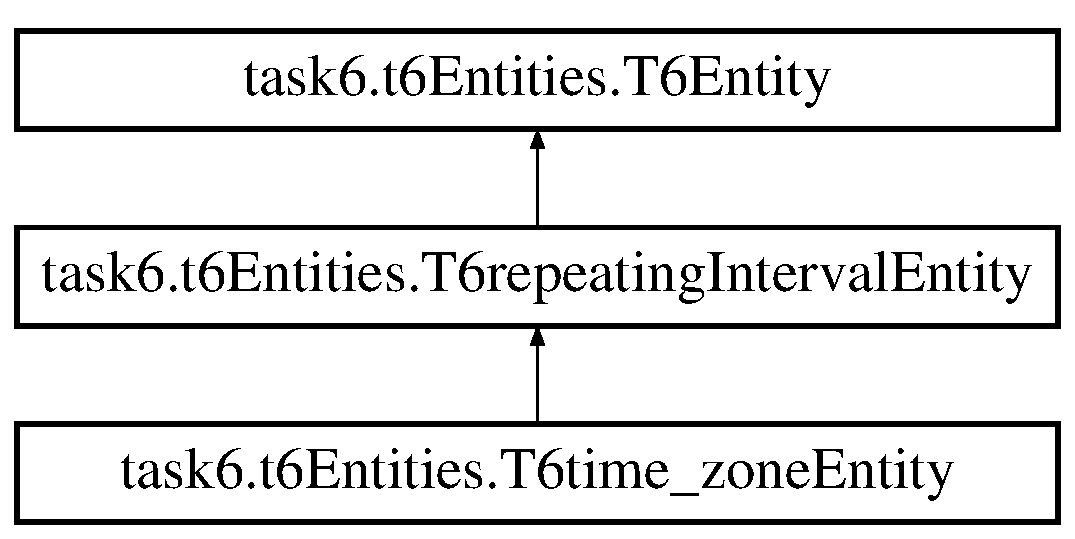
\includegraphics[height=3.000000cm]{classtask6_1_1t6Entities_1_1T6time__zoneEntity}
\end{center}
\end{figure}
\subsection*{Public Member Functions}
\begin{DoxyCompactItemize}
\item 
def \hyperlink{classtask6_1_1t6Entities_1_1T6time__zoneEntity_aa43177bdf1b06659195cf9a7cc3eaf85}{\+\_\+\+\_\+init\+\_\+\+\_\+} (self, \hyperlink{classtask6_1_1t6Entities_1_1T6Entity_afeeced8134bb3ebe0cfecc64d0ab46a4}{id}, \hyperlink{classtask6_1_1t6Entities_1_1T6Entity_a52779e9af8864dc98e8b02fc5b9b041a}{start\+\_\+span}, \hyperlink{classtask6_1_1t6Entities_1_1T6Entity_aeb402200b156cd9562c5111dfe777b98}{end\+\_\+span})
\end{DoxyCompactItemize}
\subsection*{Additional Inherited Members}


\subsection{Detailed Description}


Definition at line 163 of file t6\+Entities.\+py.



\subsection{Constructor \& Destructor Documentation}
\mbox{\Hypertarget{classtask6_1_1t6Entities_1_1T6time__zoneEntity_aa43177bdf1b06659195cf9a7cc3eaf85}\label{classtask6_1_1t6Entities_1_1T6time__zoneEntity_aa43177bdf1b06659195cf9a7cc3eaf85}} 
\index{task6\+::t6\+Entities\+::\+T6time\+\_\+zone\+Entity@{task6\+::t6\+Entities\+::\+T6time\+\_\+zone\+Entity}!\+\_\+\+\_\+init\+\_\+\+\_\+@{\+\_\+\+\_\+init\+\_\+\+\_\+}}
\index{\+\_\+\+\_\+init\+\_\+\+\_\+@{\+\_\+\+\_\+init\+\_\+\+\_\+}!task6\+::t6\+Entities\+::\+T6time\+\_\+zone\+Entity@{task6\+::t6\+Entities\+::\+T6time\+\_\+zone\+Entity}}
\subsubsection{\texorpdfstring{\+\_\+\+\_\+init\+\_\+\+\_\+()}{\_\_init\_\_()}}
{\footnotesize\ttfamily def task6.\+t6\+Entities.\+T6time\+\_\+zone\+Entity.\+\_\+\+\_\+init\+\_\+\+\_\+ (\begin{DoxyParamCaption}\item[{}]{self,  }\item[{}]{id,  }\item[{}]{start\+\_\+span,  }\item[{}]{end\+\_\+span }\end{DoxyParamCaption})}



Definition at line 164 of file t6\+Entities.\+py.



The documentation for this class was generated from the following file\+:\begin{DoxyCompactItemize}
\item 
task6/\hyperlink{t6Entities_8py}{t6\+Entities.\+py}\end{DoxyCompactItemize}

\hypertarget{classtask6_1_1t6Entities_1_1T6TwoDigitYearOperator}{}\section{task6.\+t6\+Entities.\+T6\+Two\+Digit\+Year\+Operator Class Reference}
\label{classtask6_1_1t6Entities_1_1T6TwoDigitYearOperator}\index{task6.\+t6\+Entities.\+T6\+Two\+Digit\+Year\+Operator@{task6.\+t6\+Entities.\+T6\+Two\+Digit\+Year\+Operator}}
Inheritance diagram for task6.\+t6\+Entities.\+T6\+Two\+Digit\+Year\+Operator\+:\begin{figure}[H]
\begin{center}
\leavevmode
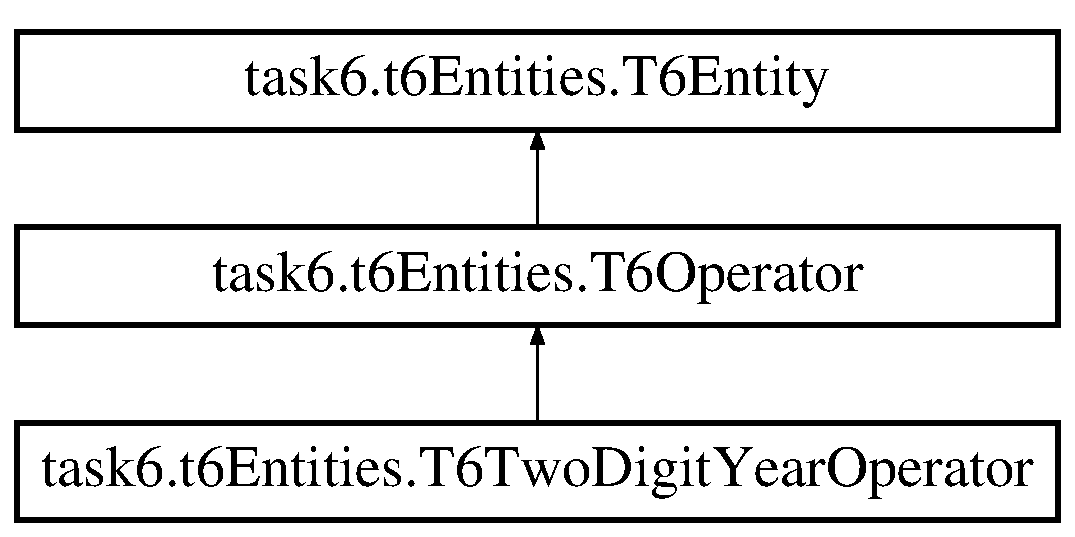
\includegraphics[height=3.000000cm]{classtask6_1_1t6Entities_1_1T6TwoDigitYearOperator}
\end{center}
\end{figure}
\subsection*{Public Member Functions}
\begin{DoxyCompactItemize}
\item 
def \hyperlink{classtask6_1_1t6Entities_1_1T6TwoDigitYearOperator_af6730d8b56d1c70a8a65798b6eb10ce0}{\+\_\+\+\_\+init\+\_\+\+\_\+} (self, \hyperlink{classtask6_1_1t6Entities_1_1T6Entity_afeeced8134bb3ebe0cfecc64d0ab46a4}{id}, \hyperlink{classtask6_1_1t6Entities_1_1T6Entity_a52779e9af8864dc98e8b02fc5b9b041a}{start\+\_\+span}, \hyperlink{classtask6_1_1t6Entities_1_1T6Entity_aeb402200b156cd9562c5111dfe777b98}{end\+\_\+span}, \hyperlink{classtask6_1_1t6Entities_1_1T6TwoDigitYearOperator_a4942dc925e5400f3877d10b184f83321}{interval\+\_\+type}, \hyperlink{classtask6_1_1t6Entities_1_1T6TwoDigitYearOperator_a12bcb3df12dbc55a9798b07d533ff9a2}{interval}, \hyperlink{classtask6_1_1t6Entities_1_1T6TwoDigitYearOperator_ab90e3c1d93213f9719a59f5806ddf6df}{period}, \hyperlink{classtask6_1_1t6Entities_1_1T6TwoDigitYearOperator_a324e05be351f629bd65001d558ba168c}{sub\+\_\+interval})
\end{DoxyCompactItemize}
\subsection*{Public Attributes}
\begin{DoxyCompactItemize}
\item 
\hyperlink{classtask6_1_1t6Entities_1_1T6TwoDigitYearOperator_a4942dc925e5400f3877d10b184f83321}{interval\+\_\+type}
\item 
\hyperlink{classtask6_1_1t6Entities_1_1T6TwoDigitYearOperator_a12bcb3df12dbc55a9798b07d533ff9a2}{interval}
\item 
\hyperlink{classtask6_1_1t6Entities_1_1T6TwoDigitYearOperator_ab90e3c1d93213f9719a59f5806ddf6df}{period}
\item 
\hyperlink{classtask6_1_1t6Entities_1_1T6TwoDigitYearOperator_a324e05be351f629bd65001d558ba168c}{sub\+\_\+interval}
\end{DoxyCompactItemize}


\subsection{Detailed Description}


Definition at line 259 of file t6\+Entities.\+py.



\subsection{Constructor \& Destructor Documentation}
\mbox{\Hypertarget{classtask6_1_1t6Entities_1_1T6TwoDigitYearOperator_af6730d8b56d1c70a8a65798b6eb10ce0}\label{classtask6_1_1t6Entities_1_1T6TwoDigitYearOperator_af6730d8b56d1c70a8a65798b6eb10ce0}} 
\index{task6\+::t6\+Entities\+::\+T6\+Two\+Digit\+Year\+Operator@{task6\+::t6\+Entities\+::\+T6\+Two\+Digit\+Year\+Operator}!\+\_\+\+\_\+init\+\_\+\+\_\+@{\+\_\+\+\_\+init\+\_\+\+\_\+}}
\index{\+\_\+\+\_\+init\+\_\+\+\_\+@{\+\_\+\+\_\+init\+\_\+\+\_\+}!task6\+::t6\+Entities\+::\+T6\+Two\+Digit\+Year\+Operator@{task6\+::t6\+Entities\+::\+T6\+Two\+Digit\+Year\+Operator}}
\subsubsection{\texorpdfstring{\+\_\+\+\_\+init\+\_\+\+\_\+()}{\_\_init\_\_()}}
{\footnotesize\ttfamily def task6.\+t6\+Entities.\+T6\+Two\+Digit\+Year\+Operator.\+\_\+\+\_\+init\+\_\+\+\_\+ (\begin{DoxyParamCaption}\item[{}]{self,  }\item[{}]{id,  }\item[{}]{start\+\_\+span,  }\item[{}]{end\+\_\+span,  }\item[{}]{interval\+\_\+type,  }\item[{}]{interval,  }\item[{}]{period,  }\item[{}]{sub\+\_\+interval }\end{DoxyParamCaption})}



Definition at line 260 of file t6\+Entities.\+py.



\subsection{Member Data Documentation}
\mbox{\Hypertarget{classtask6_1_1t6Entities_1_1T6TwoDigitYearOperator_a12bcb3df12dbc55a9798b07d533ff9a2}\label{classtask6_1_1t6Entities_1_1T6TwoDigitYearOperator_a12bcb3df12dbc55a9798b07d533ff9a2}} 
\index{task6\+::t6\+Entities\+::\+T6\+Two\+Digit\+Year\+Operator@{task6\+::t6\+Entities\+::\+T6\+Two\+Digit\+Year\+Operator}!interval@{interval}}
\index{interval@{interval}!task6\+::t6\+Entities\+::\+T6\+Two\+Digit\+Year\+Operator@{task6\+::t6\+Entities\+::\+T6\+Two\+Digit\+Year\+Operator}}
\subsubsection{\texorpdfstring{interval}{interval}}
{\footnotesize\ttfamily task6.\+t6\+Entities.\+T6\+Two\+Digit\+Year\+Operator.\+interval}



Definition at line 263 of file t6\+Entities.\+py.

\mbox{\Hypertarget{classtask6_1_1t6Entities_1_1T6TwoDigitYearOperator_a4942dc925e5400f3877d10b184f83321}\label{classtask6_1_1t6Entities_1_1T6TwoDigitYearOperator_a4942dc925e5400f3877d10b184f83321}} 
\index{task6\+::t6\+Entities\+::\+T6\+Two\+Digit\+Year\+Operator@{task6\+::t6\+Entities\+::\+T6\+Two\+Digit\+Year\+Operator}!interval\+\_\+type@{interval\+\_\+type}}
\index{interval\+\_\+type@{interval\+\_\+type}!task6\+::t6\+Entities\+::\+T6\+Two\+Digit\+Year\+Operator@{task6\+::t6\+Entities\+::\+T6\+Two\+Digit\+Year\+Operator}}
\subsubsection{\texorpdfstring{interval\+\_\+type}{interval\_type}}
{\footnotesize\ttfamily task6.\+t6\+Entities.\+T6\+Two\+Digit\+Year\+Operator.\+interval\+\_\+type}



Definition at line 262 of file t6\+Entities.\+py.

\mbox{\Hypertarget{classtask6_1_1t6Entities_1_1T6TwoDigitYearOperator_ab90e3c1d93213f9719a59f5806ddf6df}\label{classtask6_1_1t6Entities_1_1T6TwoDigitYearOperator_ab90e3c1d93213f9719a59f5806ddf6df}} 
\index{task6\+::t6\+Entities\+::\+T6\+Two\+Digit\+Year\+Operator@{task6\+::t6\+Entities\+::\+T6\+Two\+Digit\+Year\+Operator}!period@{period}}
\index{period@{period}!task6\+::t6\+Entities\+::\+T6\+Two\+Digit\+Year\+Operator@{task6\+::t6\+Entities\+::\+T6\+Two\+Digit\+Year\+Operator}}
\subsubsection{\texorpdfstring{period}{period}}
{\footnotesize\ttfamily task6.\+t6\+Entities.\+T6\+Two\+Digit\+Year\+Operator.\+period}



Definition at line 264 of file t6\+Entities.\+py.

\mbox{\Hypertarget{classtask6_1_1t6Entities_1_1T6TwoDigitYearOperator_a324e05be351f629bd65001d558ba168c}\label{classtask6_1_1t6Entities_1_1T6TwoDigitYearOperator_a324e05be351f629bd65001d558ba168c}} 
\index{task6\+::t6\+Entities\+::\+T6\+Two\+Digit\+Year\+Operator@{task6\+::t6\+Entities\+::\+T6\+Two\+Digit\+Year\+Operator}!sub\+\_\+interval@{sub\+\_\+interval}}
\index{sub\+\_\+interval@{sub\+\_\+interval}!task6\+::t6\+Entities\+::\+T6\+Two\+Digit\+Year\+Operator@{task6\+::t6\+Entities\+::\+T6\+Two\+Digit\+Year\+Operator}}
\subsubsection{\texorpdfstring{sub\+\_\+interval}{sub\_interval}}
{\footnotesize\ttfamily task6.\+t6\+Entities.\+T6\+Two\+Digit\+Year\+Operator.\+sub\+\_\+interval}



Definition at line 265 of file t6\+Entities.\+py.



The documentation for this class was generated from the following file\+:\begin{DoxyCompactItemize}
\item 
task6/\hyperlink{t6Entities_8py}{t6\+Entities.\+py}\end{DoxyCompactItemize}

\hypertarget{classtask6_1_1t6Entities_1_1T6UnionOperator}{}\section{task6.\+t6\+Entities.\+T6\+Union\+Operator Class Reference}
\label{classtask6_1_1t6Entities_1_1T6UnionOperator}\index{task6.\+t6\+Entities.\+T6\+Union\+Operator@{task6.\+t6\+Entities.\+T6\+Union\+Operator}}
Inheritance diagram for task6.\+t6\+Entities.\+T6\+Union\+Operator\+:\begin{figure}[H]
\begin{center}
\leavevmode
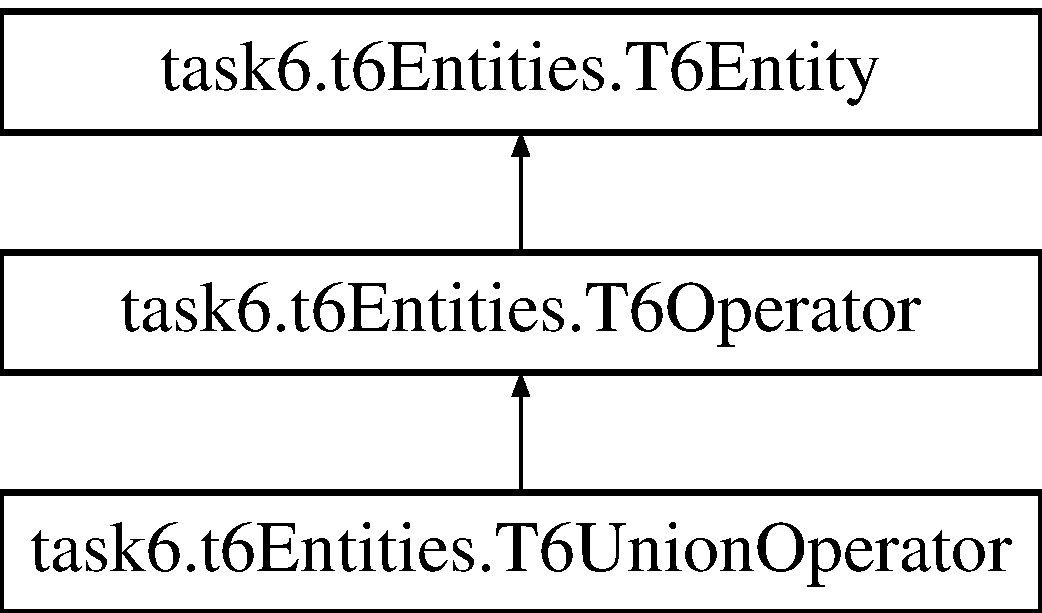
\includegraphics[height=3.000000cm]{classtask6_1_1t6Entities_1_1T6UnionOperator}
\end{center}
\end{figure}
\subsection*{Public Member Functions}
\begin{DoxyCompactItemize}
\item 
def \hyperlink{classtask6_1_1t6Entities_1_1T6UnionOperator_a781a17ffc6d31ec14fecfb2c09e63613}{\+\_\+\+\_\+init\+\_\+\+\_\+} (self, \hyperlink{classtask6_1_1t6Entities_1_1T6Entity_afeeced8134bb3ebe0cfecc64d0ab46a4}{id}, \hyperlink{classtask6_1_1t6Entities_1_1T6Entity_a52779e9af8864dc98e8b02fc5b9b041a}{start\+\_\+span}, \hyperlink{classtask6_1_1t6Entities_1_1T6Entity_aeb402200b156cd9562c5111dfe777b98}{end\+\_\+span})
\end{DoxyCompactItemize}
\subsection*{Additional Inherited Members}


\subsection{Detailed Description}


Definition at line 182 of file t6\+Entities.\+py.



\subsection{Constructor \& Destructor Documentation}
\mbox{\Hypertarget{classtask6_1_1t6Entities_1_1T6UnionOperator_a781a17ffc6d31ec14fecfb2c09e63613}\label{classtask6_1_1t6Entities_1_1T6UnionOperator_a781a17ffc6d31ec14fecfb2c09e63613}} 
\index{task6\+::t6\+Entities\+::\+T6\+Union\+Operator@{task6\+::t6\+Entities\+::\+T6\+Union\+Operator}!\+\_\+\+\_\+init\+\_\+\+\_\+@{\+\_\+\+\_\+init\+\_\+\+\_\+}}
\index{\+\_\+\+\_\+init\+\_\+\+\_\+@{\+\_\+\+\_\+init\+\_\+\+\_\+}!task6\+::t6\+Entities\+::\+T6\+Union\+Operator@{task6\+::t6\+Entities\+::\+T6\+Union\+Operator}}
\subsubsection{\texorpdfstring{\+\_\+\+\_\+init\+\_\+\+\_\+()}{\_\_init\_\_()}}
{\footnotesize\ttfamily def task6.\+t6\+Entities.\+T6\+Union\+Operator.\+\_\+\+\_\+init\+\_\+\+\_\+ (\begin{DoxyParamCaption}\item[{}]{self,  }\item[{}]{id,  }\item[{}]{start\+\_\+span,  }\item[{}]{end\+\_\+span }\end{DoxyParamCaption})}



Definition at line 183 of file t6\+Entities.\+py.



The documentation for this class was generated from the following file\+:\begin{DoxyCompactItemize}
\item 
task6/\hyperlink{t6Entities_8py}{t6\+Entities.\+py}\end{DoxyCompactItemize}

\hypertarget{classtask6_1_1t6Entities_1_1T6WeekOfYearEntity}{}\section{task6.\+t6\+Entities.\+T6\+Week\+Of\+Year\+Entity Class Reference}
\label{classtask6_1_1t6Entities_1_1T6WeekOfYearEntity}\index{task6.\+t6\+Entities.\+T6\+Week\+Of\+Year\+Entity@{task6.\+t6\+Entities.\+T6\+Week\+Of\+Year\+Entity}}
Inheritance diagram for task6.\+t6\+Entities.\+T6\+Week\+Of\+Year\+Entity\+:\begin{figure}[H]
\begin{center}
\leavevmode
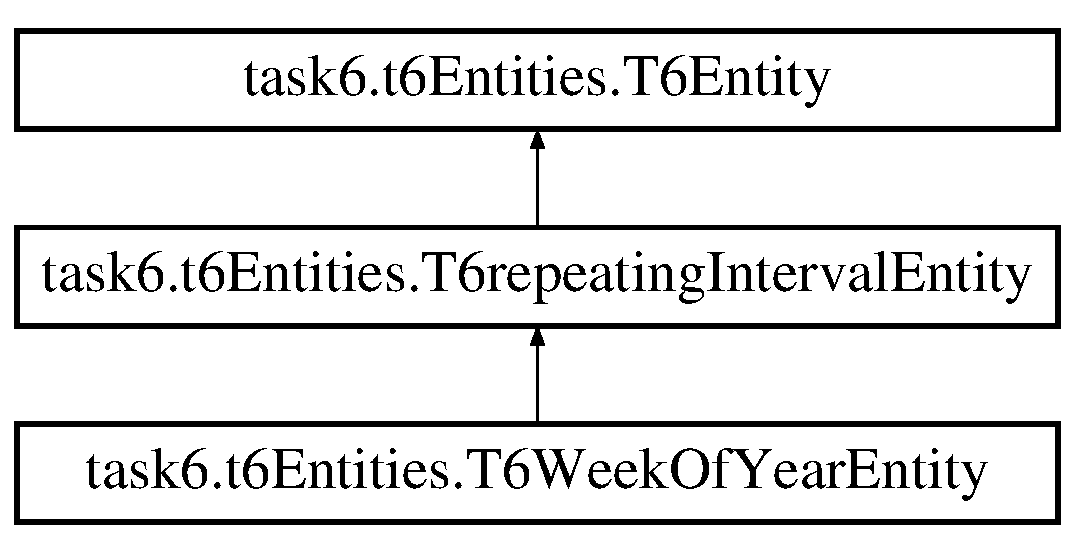
\includegraphics[height=3.000000cm]{classtask6_1_1t6Entities_1_1T6WeekOfYearEntity}
\end{center}
\end{figure}
\subsection*{Public Member Functions}
\begin{DoxyCompactItemize}
\item 
def \hyperlink{classtask6_1_1t6Entities_1_1T6WeekOfYearEntity_a383f784d6fe9b9d9cb7748b192f2cfc8}{\+\_\+\+\_\+init\+\_\+\+\_\+} (self, \hyperlink{classtask6_1_1t6Entities_1_1T6Entity_afeeced8134bb3ebe0cfecc64d0ab46a4}{id}, \hyperlink{classtask6_1_1t6Entities_1_1T6Entity_a52779e9af8864dc98e8b02fc5b9b041a}{start\+\_\+span}, \hyperlink{classtask6_1_1t6Entities_1_1T6Entity_aeb402200b156cd9562c5111dfe777b98}{end\+\_\+span}, \hyperlink{classtask6_1_1t6Entities_1_1T6WeekOfYearEntity_a4174bf8c3d14fa8c625130a7108d2d2d}{sub\+\_\+interval}, \hyperlink{classtask6_1_1t6Entities_1_1T6WeekOfYearEntity_a1fc34a92a9053036d2885b4a84e6eae6}{number}, \hyperlink{classtask6_1_1t6Entities_1_1T6WeekOfYearEntity_a98237ac4ba6e2aab8c0ae582452f3839}{modifier})
\end{DoxyCompactItemize}
\subsection*{Public Attributes}
\begin{DoxyCompactItemize}
\item 
\hyperlink{classtask6_1_1t6Entities_1_1T6WeekOfYearEntity_a4174bf8c3d14fa8c625130a7108d2d2d}{sub\+\_\+interval}
\item 
\hyperlink{classtask6_1_1t6Entities_1_1T6WeekOfYearEntity_a1fc34a92a9053036d2885b4a84e6eae6}{number}
\item 
\hyperlink{classtask6_1_1t6Entities_1_1T6WeekOfYearEntity_a98237ac4ba6e2aab8c0ae582452f3839}{modifier}
\end{DoxyCompactItemize}


\subsection{Detailed Description}


Definition at line 94 of file t6\+Entities.\+py.



\subsection{Constructor \& Destructor Documentation}
\mbox{\Hypertarget{classtask6_1_1t6Entities_1_1T6WeekOfYearEntity_a383f784d6fe9b9d9cb7748b192f2cfc8}\label{classtask6_1_1t6Entities_1_1T6WeekOfYearEntity_a383f784d6fe9b9d9cb7748b192f2cfc8}} 
\index{task6\+::t6\+Entities\+::\+T6\+Week\+Of\+Year\+Entity@{task6\+::t6\+Entities\+::\+T6\+Week\+Of\+Year\+Entity}!\+\_\+\+\_\+init\+\_\+\+\_\+@{\+\_\+\+\_\+init\+\_\+\+\_\+}}
\index{\+\_\+\+\_\+init\+\_\+\+\_\+@{\+\_\+\+\_\+init\+\_\+\+\_\+}!task6\+::t6\+Entities\+::\+T6\+Week\+Of\+Year\+Entity@{task6\+::t6\+Entities\+::\+T6\+Week\+Of\+Year\+Entity}}
\subsubsection{\texorpdfstring{\+\_\+\+\_\+init\+\_\+\+\_\+()}{\_\_init\_\_()}}
{\footnotesize\ttfamily def task6.\+t6\+Entities.\+T6\+Week\+Of\+Year\+Entity.\+\_\+\+\_\+init\+\_\+\+\_\+ (\begin{DoxyParamCaption}\item[{}]{self,  }\item[{}]{id,  }\item[{}]{start\+\_\+span,  }\item[{}]{end\+\_\+span,  }\item[{}]{sub\+\_\+interval,  }\item[{}]{number,  }\item[{}]{modifier }\end{DoxyParamCaption})}



Definition at line 95 of file t6\+Entities.\+py.



\subsection{Member Data Documentation}
\mbox{\Hypertarget{classtask6_1_1t6Entities_1_1T6WeekOfYearEntity_a98237ac4ba6e2aab8c0ae582452f3839}\label{classtask6_1_1t6Entities_1_1T6WeekOfYearEntity_a98237ac4ba6e2aab8c0ae582452f3839}} 
\index{task6\+::t6\+Entities\+::\+T6\+Week\+Of\+Year\+Entity@{task6\+::t6\+Entities\+::\+T6\+Week\+Of\+Year\+Entity}!modifier@{modifier}}
\index{modifier@{modifier}!task6\+::t6\+Entities\+::\+T6\+Week\+Of\+Year\+Entity@{task6\+::t6\+Entities\+::\+T6\+Week\+Of\+Year\+Entity}}
\subsubsection{\texorpdfstring{modifier}{modifier}}
{\footnotesize\ttfamily task6.\+t6\+Entities.\+T6\+Week\+Of\+Year\+Entity.\+modifier}



Definition at line 99 of file t6\+Entities.\+py.

\mbox{\Hypertarget{classtask6_1_1t6Entities_1_1T6WeekOfYearEntity_a1fc34a92a9053036d2885b4a84e6eae6}\label{classtask6_1_1t6Entities_1_1T6WeekOfYearEntity_a1fc34a92a9053036d2885b4a84e6eae6}} 
\index{task6\+::t6\+Entities\+::\+T6\+Week\+Of\+Year\+Entity@{task6\+::t6\+Entities\+::\+T6\+Week\+Of\+Year\+Entity}!number@{number}}
\index{number@{number}!task6\+::t6\+Entities\+::\+T6\+Week\+Of\+Year\+Entity@{task6\+::t6\+Entities\+::\+T6\+Week\+Of\+Year\+Entity}}
\subsubsection{\texorpdfstring{number}{number}}
{\footnotesize\ttfamily task6.\+t6\+Entities.\+T6\+Week\+Of\+Year\+Entity.\+number}



Definition at line 98 of file t6\+Entities.\+py.

\mbox{\Hypertarget{classtask6_1_1t6Entities_1_1T6WeekOfYearEntity_a4174bf8c3d14fa8c625130a7108d2d2d}\label{classtask6_1_1t6Entities_1_1T6WeekOfYearEntity_a4174bf8c3d14fa8c625130a7108d2d2d}} 
\index{task6\+::t6\+Entities\+::\+T6\+Week\+Of\+Year\+Entity@{task6\+::t6\+Entities\+::\+T6\+Week\+Of\+Year\+Entity}!sub\+\_\+interval@{sub\+\_\+interval}}
\index{sub\+\_\+interval@{sub\+\_\+interval}!task6\+::t6\+Entities\+::\+T6\+Week\+Of\+Year\+Entity@{task6\+::t6\+Entities\+::\+T6\+Week\+Of\+Year\+Entity}}
\subsubsection{\texorpdfstring{sub\+\_\+interval}{sub\_interval}}
{\footnotesize\ttfamily task6.\+t6\+Entities.\+T6\+Week\+Of\+Year\+Entity.\+sub\+\_\+interval}



Definition at line 97 of file t6\+Entities.\+py.



The documentation for this class was generated from the following file\+:\begin{DoxyCompactItemize}
\item 
task6/\hyperlink{t6Entities_8py}{t6\+Entities.\+py}\end{DoxyCompactItemize}

\hypertarget{classtask6_1_1t6Entities_1_1T6YearEntity}{}\section{task6.\+t6\+Entities.\+T6\+Year\+Entity Class Reference}
\label{classtask6_1_1t6Entities_1_1T6YearEntity}\index{task6.\+t6\+Entities.\+T6\+Year\+Entity@{task6.\+t6\+Entities.\+T6\+Year\+Entity}}


A year interval.  


Inheritance diagram for task6.\+t6\+Entities.\+T6\+Year\+Entity\+:\begin{figure}[H]
\begin{center}
\leavevmode
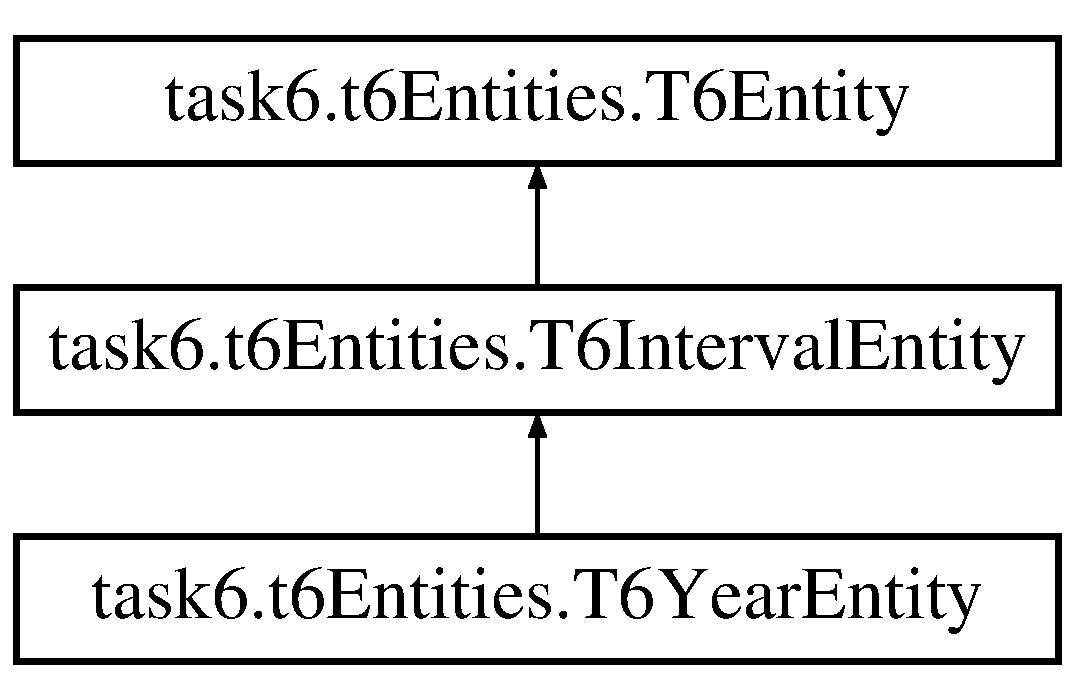
\includegraphics[height=3.000000cm]{classtask6_1_1t6Entities_1_1T6YearEntity}
\end{center}
\end{figure}
\subsection*{Public Member Functions}
\begin{DoxyCompactItemize}
\item 
def \hyperlink{classtask6_1_1t6Entities_1_1T6YearEntity_aaffc08b30d7c9ec3032a026aef3ab88d}{\+\_\+\+\_\+init\+\_\+\+\_\+} (self, \hyperlink{classtask6_1_1t6Entities_1_1T6Entity_afeeced8134bb3ebe0cfecc64d0ab46a4}{id}, \hyperlink{classtask6_1_1t6Entities_1_1T6Entity_a52779e9af8864dc98e8b02fc5b9b041a}{start\+\_\+span}, \hyperlink{classtask6_1_1t6Entities_1_1T6Entity_aeb402200b156cd9562c5111dfe777b98}{end\+\_\+span}, \hyperlink{classtask6_1_1t6Entities_1_1T6YearEntity_a5ac04f619f697c6e554af341bd3b379c}{value}, \hyperlink{classtask6_1_1t6Entities_1_1T6YearEntity_aa2f25b97805acffd72e3bcefed8f1278}{sub\+\_\+interval}=None, \hyperlink{classtask6_1_1t6Entities_1_1T6YearEntity_aaf9c16741784fcab82b65f305fb19851}{modifier}=None)
\item 
def \hyperlink{classtask6_1_1t6Entities_1_1T6YearEntity_a81385cbdd56fb486b73765bc7a01ead0}{print\+\_\+xml} (self)
\end{DoxyCompactItemize}
\subsection*{Public Attributes}
\begin{DoxyCompactItemize}
\item 
\hyperlink{classtask6_1_1t6Entities_1_1T6YearEntity_a5ac04f619f697c6e554af341bd3b379c}{value}
\item 
\hyperlink{classtask6_1_1t6Entities_1_1T6YearEntity_aa2f25b97805acffd72e3bcefed8f1278}{sub\+\_\+interval}
\item 
\hyperlink{classtask6_1_1t6Entities_1_1T6YearEntity_aaf9c16741784fcab82b65f305fb19851}{modifier}
\end{DoxyCompactItemize}


\subsection{Detailed Description}
A year interval. 


\begin{DoxyParams}{Parameters}
{\em value} & Which year \\
\hline
{\em sub\+\_\+interval} & The associated sub-\/interval \\
\hline
{\em modifier} & Any modifiers, sometimes \char`\"{}approx\char`\"{} \\
\hline
\end{DoxyParams}


Definition at line 62 of file t6\+Entities.\+py.



\subsection{Constructor \& Destructor Documentation}
\mbox{\Hypertarget{classtask6_1_1t6Entities_1_1T6YearEntity_aaffc08b30d7c9ec3032a026aef3ab88d}\label{classtask6_1_1t6Entities_1_1T6YearEntity_aaffc08b30d7c9ec3032a026aef3ab88d}} 
\index{task6\+::t6\+Entities\+::\+T6\+Year\+Entity@{task6\+::t6\+Entities\+::\+T6\+Year\+Entity}!\+\_\+\+\_\+init\+\_\+\+\_\+@{\+\_\+\+\_\+init\+\_\+\+\_\+}}
\index{\+\_\+\+\_\+init\+\_\+\+\_\+@{\+\_\+\+\_\+init\+\_\+\+\_\+}!task6\+::t6\+Entities\+::\+T6\+Year\+Entity@{task6\+::t6\+Entities\+::\+T6\+Year\+Entity}}
\subsubsection{\texorpdfstring{\+\_\+\+\_\+init\+\_\+\+\_\+()}{\_\_init\_\_()}}
{\footnotesize\ttfamily def task6.\+t6\+Entities.\+T6\+Year\+Entity.\+\_\+\+\_\+init\+\_\+\+\_\+ (\begin{DoxyParamCaption}\item[{}]{self,  }\item[{}]{id,  }\item[{}]{start\+\_\+span,  }\item[{}]{end\+\_\+span,  }\item[{}]{value,  }\item[{}]{sub\+\_\+interval = {\ttfamily None},  }\item[{}]{modifier = {\ttfamily None} }\end{DoxyParamCaption})}



Definition at line 63 of file t6\+Entities.\+py.



\subsection{Member Function Documentation}
\mbox{\Hypertarget{classtask6_1_1t6Entities_1_1T6YearEntity_a81385cbdd56fb486b73765bc7a01ead0}\label{classtask6_1_1t6Entities_1_1T6YearEntity_a81385cbdd56fb486b73765bc7a01ead0}} 
\index{task6\+::t6\+Entities\+::\+T6\+Year\+Entity@{task6\+::t6\+Entities\+::\+T6\+Year\+Entity}!print\+\_\+xml@{print\+\_\+xml}}
\index{print\+\_\+xml@{print\+\_\+xml}!task6\+::t6\+Entities\+::\+T6\+Year\+Entity@{task6\+::t6\+Entities\+::\+T6\+Year\+Entity}}
\subsubsection{\texorpdfstring{print\+\_\+xml()}{print\_xml()}}
{\footnotesize\ttfamily def task6.\+t6\+Entities.\+T6\+Year\+Entity.\+print\+\_\+xml (\begin{DoxyParamCaption}\item[{}]{self }\end{DoxyParamCaption})}



Definition at line 69 of file t6\+Entities.\+py.



\subsection{Member Data Documentation}
\mbox{\Hypertarget{classtask6_1_1t6Entities_1_1T6YearEntity_aaf9c16741784fcab82b65f305fb19851}\label{classtask6_1_1t6Entities_1_1T6YearEntity_aaf9c16741784fcab82b65f305fb19851}} 
\index{task6\+::t6\+Entities\+::\+T6\+Year\+Entity@{task6\+::t6\+Entities\+::\+T6\+Year\+Entity}!modifier@{modifier}}
\index{modifier@{modifier}!task6\+::t6\+Entities\+::\+T6\+Year\+Entity@{task6\+::t6\+Entities\+::\+T6\+Year\+Entity}}
\subsubsection{\texorpdfstring{modifier}{modifier}}
{\footnotesize\ttfamily task6.\+t6\+Entities.\+T6\+Year\+Entity.\+modifier}



Definition at line 67 of file t6\+Entities.\+py.

\mbox{\Hypertarget{classtask6_1_1t6Entities_1_1T6YearEntity_aa2f25b97805acffd72e3bcefed8f1278}\label{classtask6_1_1t6Entities_1_1T6YearEntity_aa2f25b97805acffd72e3bcefed8f1278}} 
\index{task6\+::t6\+Entities\+::\+T6\+Year\+Entity@{task6\+::t6\+Entities\+::\+T6\+Year\+Entity}!sub\+\_\+interval@{sub\+\_\+interval}}
\index{sub\+\_\+interval@{sub\+\_\+interval}!task6\+::t6\+Entities\+::\+T6\+Year\+Entity@{task6\+::t6\+Entities\+::\+T6\+Year\+Entity}}
\subsubsection{\texorpdfstring{sub\+\_\+interval}{sub\_interval}}
{\footnotesize\ttfamily task6.\+t6\+Entities.\+T6\+Year\+Entity.\+sub\+\_\+interval}



Definition at line 66 of file t6\+Entities.\+py.

\mbox{\Hypertarget{classtask6_1_1t6Entities_1_1T6YearEntity_a5ac04f619f697c6e554af341bd3b379c}\label{classtask6_1_1t6Entities_1_1T6YearEntity_a5ac04f619f697c6e554af341bd3b379c}} 
\index{task6\+::t6\+Entities\+::\+T6\+Year\+Entity@{task6\+::t6\+Entities\+::\+T6\+Year\+Entity}!value@{value}}
\index{value@{value}!task6\+::t6\+Entities\+::\+T6\+Year\+Entity@{task6\+::t6\+Entities\+::\+T6\+Year\+Entity}}
\subsubsection{\texorpdfstring{value}{value}}
{\footnotesize\ttfamily task6.\+t6\+Entities.\+T6\+Year\+Entity.\+value}



Definition at line 65 of file t6\+Entities.\+py.



The documentation for this class was generated from the following file\+:\begin{DoxyCompactItemize}
\item 
task6/\hyperlink{t6Entities_8py}{t6\+Entities.\+py}\end{DoxyCompactItemize}

\chapter{File Documentation}
\hypertarget{README_8md}{}\section{R\+E\+A\+D\+M\+E.\+md File Reference}
\label{README_8md}\index{R\+E\+A\+D\+M\+E.\+md@{R\+E\+A\+D\+M\+E.\+md}}

\hypertarget{setup_8py}{}\section{setup.\+py File Reference}
\label{setup_8py}\index{setup.\+py@{setup.\+py}}
\subsection*{Namespaces}
\begin{DoxyCompactItemize}
\item 
 \hyperlink{namespacesetup}{setup}
\end{DoxyCompactItemize}
\subsection*{Variables}
\begin{DoxyCompactItemize}
\item 
\hyperlink{namespacesetup_a9c076537d899ffd8096e58c282bb7b02}{setup.\+here} = path.\+abspath(path.\+dirname(\+\_\+\+\_\+file\+\_\+\+\_\+))
\item 
\hyperlink{namespacesetup_a443be2d01fd539bf6761aff70724d876}{setup.\+encoding}
\item 
\hyperlink{namespacesetup_a4cda9dbfb952875376a0749fe08a5bde}{setup.\+long\+\_\+description} = f.\+read()
\item 
\hyperlink{namespacesetup_ab3a7a0638d76a01367c5bc3cc699447f}{setup.\+name}
\item 
\hyperlink{namespacesetup_a2aa722b36a933088812b50ea79b97a5c}{setup.\+version}
\item 
\hyperlink{namespacesetup_aedf461ec52a946bda975938ba0b93ec0}{setup.\+description}
\item 
\hyperlink{namespacesetup_afc13124aa5c0124e84e1d965e3f4b0fb}{setup.\+url}
\item 
\hyperlink{namespacesetup_a3a57a4772d418a06835249cbade0d86a}{setup.\+author}
\item 
\hyperlink{namespacesetup_a5b08034343aa2be607722a8b315f3625}{setup.\+author\+\_\+email}
\item 
\hyperlink{namespacesetup_a8ed6f50a28bd6a8794f8e1153baa6de9}{setup.\+license}
\item 
\hyperlink{namespacesetup_abe96a9c38c1c61f9f0fdb002c482f785}{setup.\+classifiers}
\item 
\hyperlink{namespacesetup_a73ae9ecb109f0dcab6f0b6a89043c5c3}{setup.\+keywords}
\item 
\hyperlink{namespacesetup_aff2375a361fd5865c77bd9aa093be747}{setup.\+packages}
\item 
\hyperlink{namespacesetup_abead4f26b530856f858f0d44c7cf2588}{setup.\+install\+\_\+requires}
\end{DoxyCompactItemize}

\hypertarget{task6_2____init_____8py}{}\section{task6/\+\_\+\+\_\+init\+\_\+\+\_\+.py File Reference}
\label{task6_2____init_____8py}\index{task6/\+\_\+\+\_\+init\+\_\+\+\_\+.\+py@{task6/\+\_\+\+\_\+init\+\_\+\+\_\+.\+py}}
\subsection*{Namespaces}
\begin{DoxyCompactItemize}
\item 
 \hyperlink{namespacetask6}{task6}
\end{DoxyCompactItemize}

\hypertarget{test_2____init_____8py}{}\section{test/\+\_\+\+\_\+init\+\_\+\+\_\+.py File Reference}
\label{test_2____init_____8py}\index{test/\+\_\+\+\_\+init\+\_\+\+\_\+.\+py@{test/\+\_\+\+\_\+init\+\_\+\+\_\+.\+py}}
\subsection*{Namespaces}
\begin{DoxyCompactItemize}
\item 
 \hyperlink{namespacetest}{test}
\end{DoxyCompactItemize}

\hypertarget{sutime_8py}{}\section{task6/sutime.py File Reference}
\label{sutime_8py}\index{task6/sutime.\+py@{task6/sutime.\+py}}
\subsection*{Classes}
\begin{DoxyCompactItemize}
\item 
class \hyperlink{classtask6_1_1sutime_1_1SUTime}{task6.\+sutime.\+S\+U\+Time}
\end{DoxyCompactItemize}
\subsection*{Namespaces}
\begin{DoxyCompactItemize}
\item 
 \hyperlink{namespacetask6_1_1sutime}{task6.\+sutime}
\end{DoxyCompactItemize}

\hypertarget{sutime__wrapper_8py}{}\section{task6/sutime\+\_\+wrapper.py File Reference}
\label{sutime__wrapper_8py}\index{task6/sutime\+\_\+wrapper.\+py@{task6/sutime\+\_\+wrapper.\+py}}
\subsection*{Namespaces}
\begin{DoxyCompactItemize}
\item 
 \hyperlink{namespacetask6_1_1sutime__wrapper}{task6.\+sutime\+\_\+wrapper}
\end{DoxyCompactItemize}
\subsection*{Functions}
\begin{DoxyCompactItemize}
\item 
def \hyperlink{namespacetask6_1_1sutime__wrapper_af4cac751d594757efbe539a28850ff28}{task6.\+sutime\+\_\+wrapper.\+call\+S\+U\+Time\+Parse} (file\+\_\+path)
\begin{DoxyCompactList}\small\item\em call\+S\+U\+T\+I\+M\+E\+Parse() Function Purpose\+: Takes in raw text file and performs S\+U\+Time\textquotesingle{}s algorithm on \#it and returns it in J\+S\+ON format. \end{DoxyCompactList}\end{DoxyCompactItemize}

\hypertarget{t6Entities_8py}{}\section{task6/t6\+Entities.py File Reference}
\label{t6Entities_8py}\index{task6/t6\+Entities.\+py@{task6/t6\+Entities.\+py}}
\subsection*{Classes}
\begin{DoxyCompactItemize}
\item 
class \hyperlink{classtask6_1_1t6Entities_1_1t6Entity}{task6.\+t6\+Entities.\+t6\+Entity}
\begin{DoxyCompactList}\small\item\em Programmer Name\+: Luke Maffey Date\+: 9/19/17 Module Purpose\+: Class definitions for all Time\+Norm entities -\/ Intervals, Periods, Repeating-\/\+Intervals, and Operators. \end{DoxyCompactList}\item 
class \hyperlink{classtask6_1_1t6Entities_1_1t6IntervalEntity}{task6.\+t6\+Entities.\+t6\+Interval\+Entity}
\item 
class \hyperlink{classtask6_1_1t6Entities_1_1t6PeriodEntity}{task6.\+t6\+Entities.\+t6\+Period\+Entity}
\item 
class \hyperlink{classtask6_1_1t6Entities_1_1t6RepeatingIntervalEntity}{task6.\+t6\+Entities.\+t6\+Repeating\+Interval\+Entity}
\item 
class \hyperlink{classtask6_1_1t6Entities_1_1t6Operator}{task6.\+t6\+Entities.\+t6\+Operator}
\end{DoxyCompactItemize}
\subsection*{Namespaces}
\begin{DoxyCompactItemize}
\item 
 \hyperlink{namespacetask6_1_1t6Entities}{task6.\+t6\+Entities}
\end{DoxyCompactItemize}

\hypertarget{utils_8py}{}\section{task6/utils.py File Reference}
\label{utils_8py}\index{task6/utils.\+py@{task6/utils.\+py}}
\subsection*{Namespaces}
\begin{DoxyCompactItemize}
\item 
 \hyperlink{namespacetask6_1_1utils}{task6.\+utils}
\end{DoxyCompactItemize}
\subsection*{Functions}
\begin{DoxyCompactItemize}
\item 
def \hyperlink{namespacetask6_1_1utils_a515e86e4cb66853a491562c4dd7935b1}{task6.\+utils.\+get\+Whitespace\+Spans} (file\+\_\+path)
\begin{DoxyCompactList}\small\item\em \hyperlink{namespacetask6_1_1utils_a515e86e4cb66853a491562c4dd7935b1}{get\+Whitespace\+Spans()} Function Purpose\+: Pasrses a text file to idenitfy all tokens seperated by white space with their original file span coordinates. \end{DoxyCompactList}\end{DoxyCompactItemize}

\hypertarget{test_2test_8py}{}\section{test/test.py File Reference}
\label{test_2test_8py}\index{test/test.\+py@{test/test.\+py}}
\subsection*{Namespaces}
\begin{DoxyCompactItemize}
\item 
 \hyperlink{namespacetest_1_1test}{test.\+test}
\end{DoxyCompactItemize}
\subsection*{Variables}
\begin{DoxyCompactItemize}
\item 
\hyperlink{namespacetest_1_1test_ac6940ca06224277c08c299101b3296b4}{test.\+test.\+r}
\item 
\hyperlink{namespacetest_1_1test_a85ce85cce39e2fad621db9c70186235a}{test.\+test.\+t}
\item 
\hyperlink{namespacetest_1_1test_a4e3f76bc561357031de5269619280f91}{test.\+test.\+s}
\end{DoxyCompactItemize}

\hypertarget{test_8py}{}\section{test.\+py File Reference}
\label{test_8py}\index{test.\+py@{test.\+py}}
\subsection*{Namespaces}
\begin{DoxyCompactItemize}
\item 
 \hyperlink{namespacetest}{test}
\end{DoxyCompactItemize}
\subsection*{Variables}
\begin{DoxyCompactItemize}
\item 
\hyperlink{namespacetest_ac1f92ca15306aee561188e0f37aabc66}{test.\+r}
\item 
\hyperlink{namespacetest_ae9ebdaf735944736b55d720cfe9c3e02}{test.\+t}
\item 
\hyperlink{namespacetest_a91a88df52e09e64ff8cc9e5d8277c8d4}{test.\+s}
\end{DoxyCompactItemize}

%--- End generated contents ---

% Index
\backmatter
\newpage
\phantomsection
\clearemptydoublepage
\addcontentsline{toc}{chapter}{Index}
\printindex

\end{document}
